% /*
%  * ----------------------------------------------------------------------------
%  * "THE BEER-WARE LICENSE" (Revision 42):
%  * Julian Klaiber and Severin Dellsperger wrote this file. As long as you retain this notice you
%  * can do whatever you want with this stuff. If we meet some day, and you think
%  * this stuff is worth it, you can buy us a beer in return.
%  * ----------------------------------------------------------------------------
%  */

% Template Informationen
\documentclass[
a4paper,
oneside,
10pt,
fleqn,
headsepline,
toc=listofnumbered, 
bibliography=totocnumbered]{scrartcl}

% deutsche Trennmuster etc.
\usepackage[T1]{fontenc}
\usepackage[utf8]{inputenc}
\usepackage[english, ngerman]{babel} % \selectlanguage{english} if  needed
\usepackage{lmodern} % use modern latin fonts

% Custom commands
\newcommand{\GITHUB}{https://github.com/jklaiber/HSR}
\newcommand{\LICENSEURL}{https://en.wikipedia.org/wiki/Beerware}
\newcommand{\LICENSE}{
"THE BEER-WARE LICENSE" (Revision 42):
Julian Klaiber and Severin Dellsperger wrote this file. As long as you retain this notice you
can do whatever you want with this stuff. If we meet some day, and you think
this stuff is worth it, you can buy us a beer in return.
}

% Jede Überschrift 1 auf neuer Seite
\let\stdsection\section
\renewcommand\section{\clearpage\stdsection}

% Multiple Authors
\usepackage{authblk}

% Include external pdf
\usepackage{pdfpages}

% Layout / Seitenränder
\usepackage{geometry}

% Inhaltsverzeichnis
\usepackage{makeidx} 
\makeindex

\usepackage{url}
\usepackage[pdfborder={0 0 0}]{hyperref}
\usepackage[all]{hypcap}
\usepackage{hyperxmp} % for license metadata

% Glossar und Abkürzungsverzeichnis
\usepackage[acronym,toc,nopostdot]{glossaries}
\setglossarystyle{altlist}
\usepackage{xparse}
\DeclareDocumentCommand{\newdualentry}{ O{} O{} m m m m } {
	\newglossaryentry{gls-#3}{
		name={#4 : #5},
		text={#5\glsadd{#3}},
		description={#6},
		#1
	}
	\makeglossaries
	\newacronym[see={[Siehe:]{gls-#3}},#2]{#3}{#4}{#5\glsadd{gls-#3}}
}
\makeglossaries

% Mathematik
\usepackage{amsmath}
\usepackage{amssymb}
\usepackage{amsfonts}
\usepackage{enumitem}

% Images
\usepackage{graphicx}
\graphicspath{{images/}} % default paths

% Boxes
\usepackage{fancybox}

%Tables
\usepackage{tabu}
\usepackage{booktabs} % toprule, midrule, bottomrule
\usepackage{array} % for matrix tables
\usepackage{multicol} %multicol

% Header and footer
\usepackage{scrlayer-scrpage}
\setkomafont{pagehead}{\normalfont}
\setkomafont{pagefoot}{\normalfont}
\automark*{section}
\clearpairofpagestyles
\ihead{\headmark}
\ohead{\AUTHOR}
\cfoot{\pagemark}

% Pseudocode
\usepackage{algorithmic}
\usepackage[linesnumbered,ruled]{algorithm2e}

% Code Listings
\usepackage{listings}
\usepackage{color}
\usepackage{beramono}

\definecolor{bluekeywords}{rgb}{0,0,1}
\definecolor{greencomments}{rgb}{0,0.5,0}
\definecolor{redstrings}{rgb}{0.64,0.08,0.08}
\definecolor{xmlcomments}{rgb}{0.5,0.5,0.5}
\definecolor{types}{rgb}{0.17,0.57,0.68}

\lstdefinestyle{visual-studio-style}{
	language=[Sharp]C,
	columns=flexible,
	showstringspaces=false,
	basicstyle=\footnotesize\ttfamily, 
	commentstyle=\color{greencomments},
	morekeywords={partial, var, value, get, set},
	keywordstyle=\bfseries\color{bluekeywords},
	stringstyle=\color{redstrings},
	breaklines=true,
	breakatwhitespace=true,
	tabsize=4,
	numbers=left,
	numberstyle=\tiny\color{black},
	frame=lines,
	showspaces=false,
	showtabs=false,
	escapeinside={£}{£},
}

\definecolor{DarkPurple}{rgb}{0.4, 0.1, 0.4}
\definecolor{DarkCyan}{rgb}{0.0, 0.5, 0.4}
\definecolor{LightLime}{rgb}{0.3, 0.5, 0.4}
\definecolor{Blue}{rgb}{0.0, 0.0, 1.0}

\lstdefinestyle{cevelop-style}{
	language=C++,  
	columns=flexible,
	showstringspaces=false,     
	basicstyle=\footnotesize\ttfamily, 
	keywordstyle=\bfseries\color{DarkPurple},
	commentstyle=\color{LightLime},
	stringstyle=\color{Blue}, 
	escapeinside={£}{£}, % latex scope within code      
	breaklines=true,
	breakatwhitespace=true,
	showspaces=false,
	showtabs=false,
	tabsize=4,
	morekeywords={include,ifndef,define},
	numbers=left,
	numberstyle=\tiny\color{black},
	frame=lines,
}

\lstdefinestyle{eclipse-style}{
	language=Java,  
	columns=flexible,
	showstringspaces=false,     
	basicstyle=\footnotesize\ttfamily, 
	keywordstyle=\bfseries\color{DarkPurple},
	commentstyle=\color{LightLime},
	stringstyle=\color{Blue}, 
	escapeinside={£}{£}, % latex scope within code      
	breaklines=true,
	breakatwhitespace=true,
	showspaces=false,
	showtabs=false,
	tabsize=4,
	morekeywords={length},
	numbers=left,
	numberstyle=\tiny\color{black},
	frame=lines,
}
\lstset{style=eclipse-style}



% Theorems \begin{mytheo}{title}{label}
\usepackage{tcolorbox}
\tcbuselibrary{theorems}
\newtcbtheorem[number within=section]{definiton}{Definition}%
{fonttitle=\bfseries}{def}
\newtcbtheorem[number within=section]{remember}{Merke}%
{fonttitle=\bfseries}{rem}
\newtcbtheorem[number within=section]{hint}{Hinweis}%
{fonttitle=\bfseries}{hnt}

% Colors
\definecolor{strings}{HTML}{448c25}
\definecolor{comments}{HTML}{aaaaaa}
\definecolor{keywords}{HTML}{aa3d8c}
\definecolor{background}{HTML}{f4f4f4}
\definecolor{numbers}{HTML}{a884e0}

% Default style
\lstdefinestyle{default}{
    backgroundcolor=\color{background},
    basicstyle=\ttfamily\small,
    breakatwhitespace=true,
    breaklines=true,
    commentstyle=\color{comments},
    deletekeywords={},
    escapeinside={}{},
    extendedchars=true,
    frame=lines,
    keepspaces=true,
    keywordstyle=\color{keywords},
    morekeywords={},
    numbers=left,
    numberstyle=\ttfamily\color{numbers},
    rulecolor=\color{numbers},
    showspaces=false,
    showstringspaces=false,
    showtabs=false,
    stepnumber=1,
    stringstyle=\color{strings},
    tabsize=2,
}
\lstset{
    style=default,
    columns=fullflexible
}

% Language cisco-config
\lstdefinelanguage{cisco-config}{
    morekeywords={no,ip,ipv6,int,interface},
    morecomment=[l][\color{comments}]{!},
    numbers=none
}

% Language cisco-teminal
\lstdefinelanguage{cisco-terminal}{
    morecomment=[l][\color{strings}]{\#},
    morecomment=[l][\color{strings}]{>},
    numbers=none
}

\lstdefinelanguage{bash}{
    numbers=none
}

\makeatletter
\@addtoreset{section}{part}
\makeatother

% Boxes
\tcbuselibrary{most}

\usepackage{fontawesome}

% \cmd{...}
\newcommand{\cmd}[1]{\texttt{#1}}

% Info Box
\definecolor{infobar}{HTML}{02cefc}
\definecolor{infobackground}{HTML}{baf0fc}
\newcommand{\info}[2]{
    \begin{tcolorbox}[
        arc = 0mm,
        boxrule = 0pt,
        breakable,
        before skip=11pt,
        before skip=11pt,
        title = \faInfo~#1,
        fonttitle = \sffamily\bfseries,
        coltitle = white,
        colbacktitle = infobar,
        colback = infobackground,
        toptitle=2mm,
        bottomtitle=2mm,
        top=4mm,
        bottom=4mm
    ]
    #2
    \end{tcolorbox}
}

% Warning Box
\definecolor{warnbar}{HTML}{f90053}
\definecolor{warnbackground}{HTML}{fcc4d7}
\newcommand{\warn}[2]{
    \begin{tcolorbox}[
        arc = 0mm,
        boxrule = 0pt,
        breakable,
        before skip=11pt,
        before skip=11pt,
        title = \faWarning~#1,
        fonttitle = \sffamily\bfseries,
        coltitle = white,
        colbacktitle = warnbar,
        colback = warnbackground,
        toptitle=2mm,
        bottomtitle=2mm,
        top=4mm,
        bottom=4mm
    ]
    #2
    \end{tcolorbox}
}

% Login Information Box
\definecolor{loginbar}{HTML}{FA8A05}
\definecolor{loginbackground}{HTML}{F3D4AF}
\newcommand{\login}[2]{
    \begin{tcolorbox}[
        arc = 0mm,
        boxrule = 0pt,
        breakable,
        before skip=11pt,
        before skip=11pt,
        title = \faKey~#1,
        fonttitle = \sffamily\bfseries,
        coltitle = white,
        colbacktitle = loginbar,
        colback = loginbackground,
        toptitle=2mm,
        bottomtitle=2mm,
        top=4mm,
        bottom=4mm
    ]
    #2
    \end{tcolorbox}
}

\definecolor{settingborder}{HTML}{0066CC}
\definecolor{settingcontent}{HTML}{E5F2FA}
\newcommand{\setting}[1]{
    \begin{tcolorbox}[
        colback = settingcontent,
        colframe = settingborder
    ]
    You can find the settings under: \\
    \textbf{\clicks{~#1}}
    \end{tcolorbox}
}

\definecolor{configurationborder}{HTML}{005700}
\definecolor{configurationcontent}{HTML}{e6ffcc}
\newcommand{\configuration}[2]{
    \begin{tcolorbox}[
        colback = configurationcontent,
        colframe = configurationborder
    ]
    \textbf{Configuration:}\\
    To reach an output like below you only have to add/change the following parameters 
    ~#1
    You can find the settings under: \\
    \textbf{\clicks{~#2}}
    \end{tcolorbox}
}


\usepackage{multirow}

% URLs
\urlstyle{rm}
\definecolor{link}{HTML}{0450f2}
\hypersetup{
    colorlinks,
    allcolors=.,
    urlcolor=link,
}

% \url[display]{url} or \url{url}
\renewcommand{\url}[2][]{%
    \ifstrempty{#1}{%
        \burlalt{#2}{#2}%
    }{%
        \burlalt{#1}{#2}%
    }%
}

% Clicks
\newcommand{\clicks}[1]{%
    $\foreach \n [count=\ni] in {#1}{%
        \ifnum\ni=1%
            \textit{\n}%
        \else%
            \rightarrow \textit{\n}%
        \fi%
    }$%
}

% Keystrokes
\newcommand{\keys}[1]{%
    $\foreach \n [count=\ni] in {#1}{%
        \ifnum\ni=1%
            \textit{\n}%
        \else%
            + \textit{\n}%
        \fi%
    }$%
}

% Dokumentinformationen
\newcommand{\INSTITUTE}{Hochschule für Technik Rapperswil}
\newcommand{\SUBJECT}{Zusammenfassung}
\newcommand{\TITLE}{Informationssicherheit 2}
\newcommand{\AUTHORONE}{Julian Klaiber}
\newcommand{\AUTHORTWO}{Severin Dellsperger}

% Titelseite einfügen
% pdf metadata
\hypersetup{
	pdfauthor={\AUTHOR},
	pdftitle={\SUBJECT \TITLE},
	pdfcopyright={\LICENSE},
	pdflicenseurl={\LICENSEURL}
}

\begin{document}
	
\begin{titlepage}

\newcommand{\HRule}{\rule{\linewidth}{0.5mm}} % Defines a new command for the horizontal lines, change thickness here

\center % Center everything on the page
 
%----------------------------------------------------------------------------------------
%	HEADING SECTIONS
%----------------------------------------------------------------------------------------

\textsc{\LARGE \INSTITUTE}\\[1.5cm] % Name of your university/college
\textsc{\Large \SUBJECT}\\[0.5cm] % Major heading such as course name

%----------------------------------------------------------------------------------------
%	TITLE SECTION
%----------------------------------------------------------------------------------------

\HRule \\[0.6cm]
{ \huge \bfseries \TITLE}\\[0.4cm] % Title of your document
\HRule \\[1.5cm]

%----------------------------------------------------------------------------------------
%	AUTHOR SECTION
%----------------------------------------------------------------------------------------

\begin{minipage}{0.4\textwidth}
\begin{flushleft} \large
\emph{Author:}\\
\AUTHORONE % Your name
\end{flushleft}
\end{minipage}
~
\begin{minipage}{0.4\textwidth}
\begin{flushright} \large
\emph{} \\
\AUTHORTWO
\end{flushright}
\end{minipage}\\[2cm]

%----------------------------------------------------------------------------------------
%	DATE SECTION
%----------------------------------------------------------------------------------------

{\large \today}\\[2cm] % Date, change the \today to a set date if you want to be precise

%----------------------------------------------------------------------------------------
%	LOGO SECTION
%----------------------------------------------------------------------------------------


\includegraphics[width=10cm,height=5cm,keepaspectratio]{ressources/hsr_logo.jpg}\\[1cm] 
 
%----------------------------------------------------------------------------------------

\vfill % Fill the rest of the page with whitespace

\end{titlepage} 	


% Inhaltsverzeichnis einfügen
\tableofcontents

% Start der Dokumentation


\section{Grundlagen}
\subsection{OSI Stack}
\begin{figure}[h]
\centering
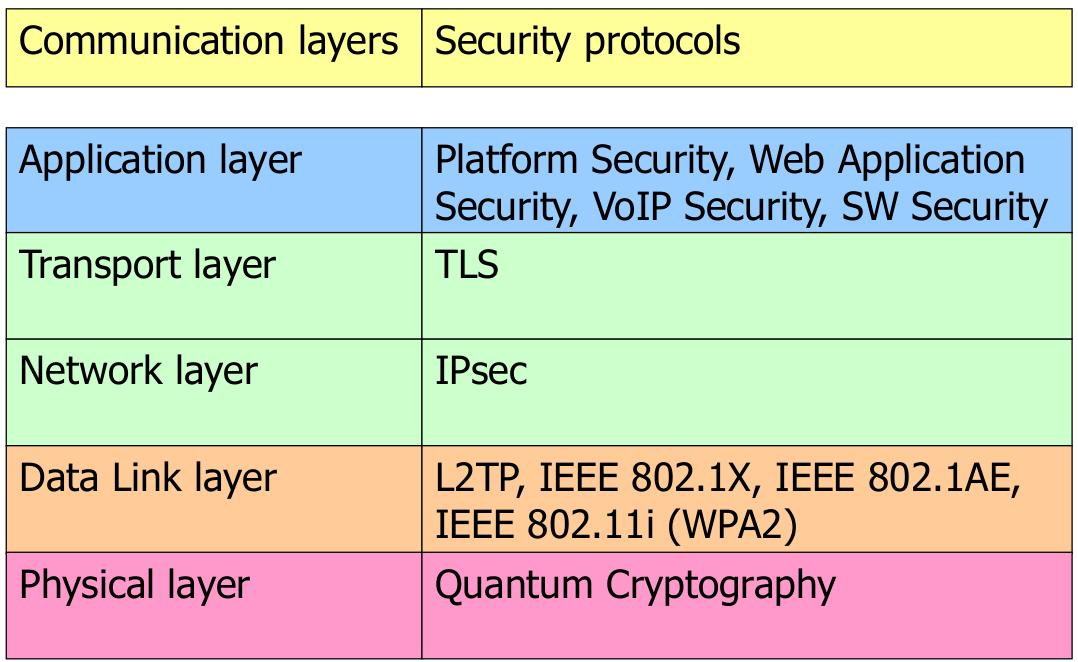
\includegraphics[width=0.7\linewidth]{images/sec_osi_stack}
\caption{OSI Stack}
%\label{fig:secosistack}
\end{figure}

\begin{itemize}
    \item L2TP: \textit{Layer 2 Tunneling Protocol}
    \item IEEE 802.1X: \textit{Standard Authentifizierungsmethode für Netzwerke - Stichwort eduroam, Radius}
    \item IEEE 802.1AE \textit{MAC Security Standard - MACsec}
    \item IEEE802.11i: \textit{Sicherheitserweiterung für Wireless LAN (WPA2)}
    \item IPsec: \textit{Internet Protocol Security - Layer 3 Security)}
    \item TLS: \textit{Transport Layer Security - Layer 3 Security (Nachfolger von SSL)}
\end{itemize}


\subsection{Kryptographiesche Stärken}
\paragraph{Kryptographiesche Stärken} \hfill
\newline
\begin{minipage}[t]{1\textwidth}
    \centering
	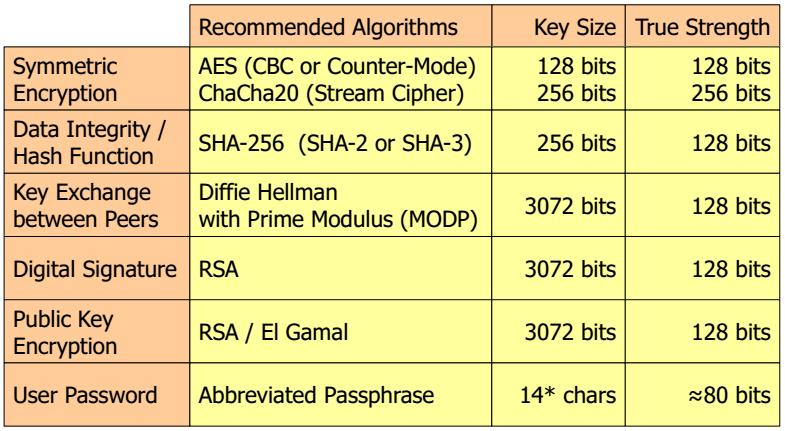
\includegraphics[width=0.7\linewidth]{images/cryptographical_strenght}
	\label{fig:cryptographicalstrenght}
\end{minipage}


\paragraph{NIST 2012 Comparative Security Strength} \hfill
\begin{hint}{NIST 2012 Compartive Security Strenght}{}
	Diese Grafiken müssen auswendig gelernt werden. Kommt garantiert an der Prüfung!
\end{hint}


\begin{minipage}[t]{1\textwidth}
    \centering
	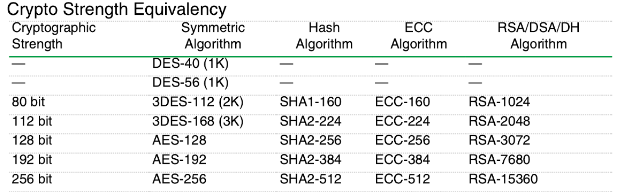
\includegraphics[width=0.9\linewidth]{images/crypto-strength-table.png}
    \caption{}
    \label{fig:keystrenghtcomparison}
\end{minipage}

\begin{minipage}[t]{1\textwidth}
    \centering
	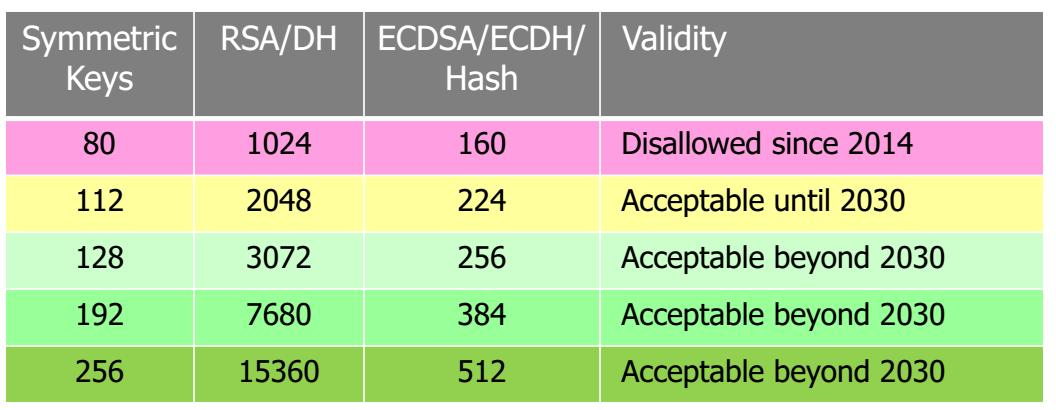
\includegraphics[width=0.7\linewidth]{images/key_strenght_comparison}
    \caption{}
    \label{fig:keystrenghtcomparison}
\end{minipage}



\paragraph{Prüfungsaufgabe HS 18/19} \hfill
\newline
\begin{minipage}[t]{1\textwidth}
    \centering
	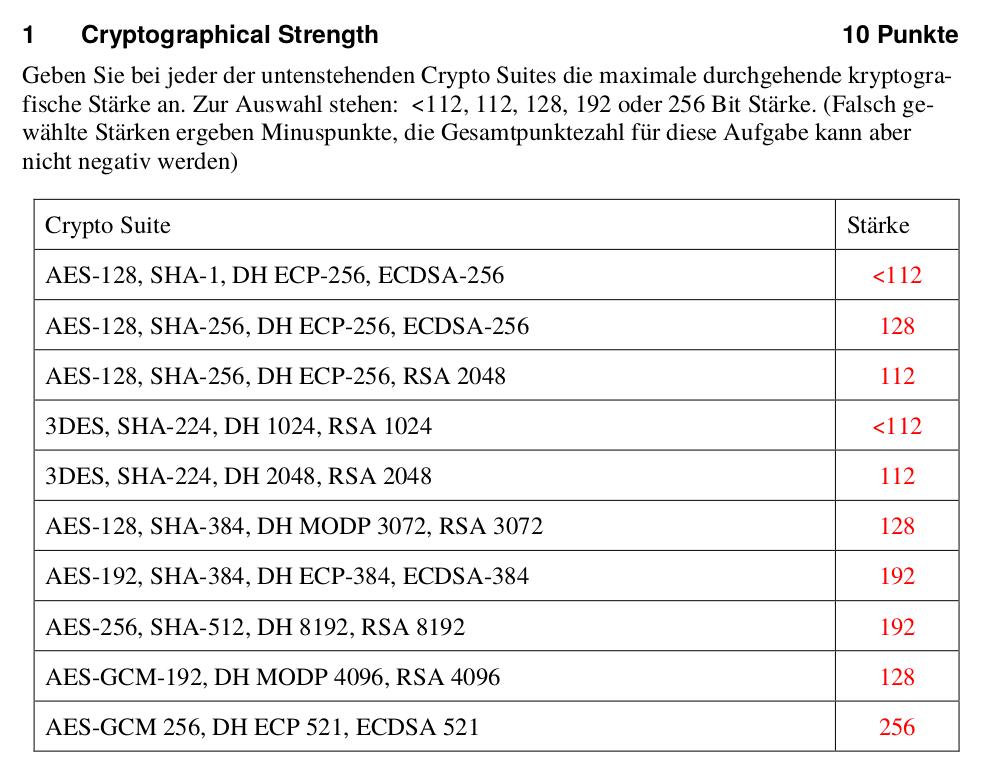
\includegraphics[width=0.95\linewidth]{images/hs18-19-crypto-strength.png}
\end{minipage}
\paragraph{Tipps zum Merken}
\begin{itemize}
    \item \textbf{AES} Kryptografische Staerke = Schluessellaenge
    \item \textbf{SHA, ECC} Kryptografische Staerke = halbe Schluessellaenge
    \item \textbf{3DES} Kryptografische Staerke = 112 Bit
    \item \textbf{RSA/DH} 1024 (80 bit), 2048 (112 bit), 3072 (128 Bit), 8192 (192 Bit), 15360 (256 Bit)
\end{itemize}

\subsection{NSA Suite B}
Die Suite A beinhaltet Algorithmen, welche die NSA als \textit{nicht für die Öffentlichkeit} bestimmt hat. Es sind extrem starke Algorithmen, welche für die Verschlüsselung von extrem sensitiven Daten, beispielsweise der NSA, verwendet werden.\\
Die Suite B ist eine Sammlung an kryptographischer Algorithmen, die 2005 von der NSA veröffentlicht wurde. Es ist eine Empfehlung der NSA, welche Algorithmen für welche Kategorie (SECRET/TOPSECRET) eingesetzt werden soll. Die Kategorie \textit{SECRET} hat dabei eine kryptographische Stärke von 128 bit, die \textit{TOPSECRET} Kategorie eine Stärke von 192 bits.

\begin{minipage}[t]{1\textwidth}
\centering
	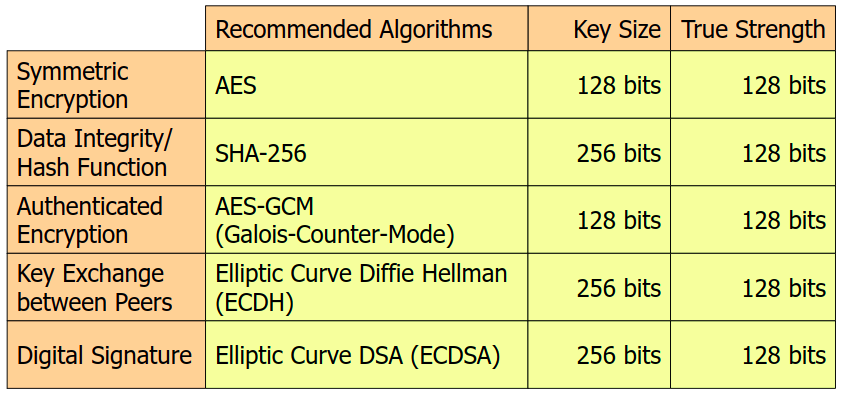
\includegraphics[width=0.8\linewidth]{images/suite-b-128.png}
\end{minipage}

\begin{minipage}[t]{1\textwidth}
\centering
	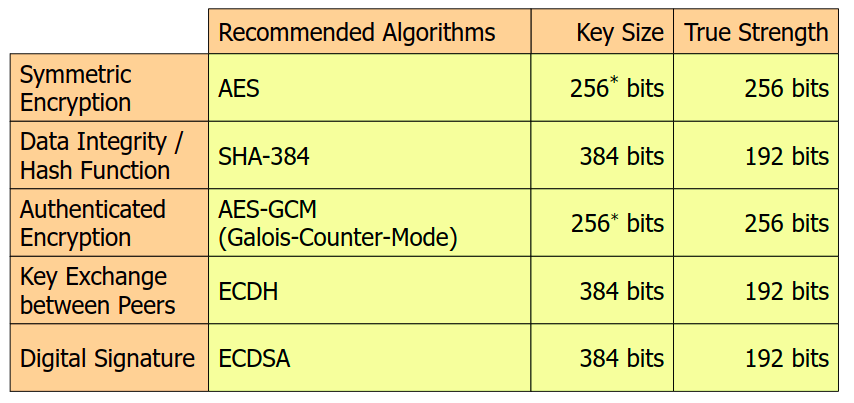
\includegraphics[width=0.8\linewidth]{images/suite-b-192.png}
\end{minipage}

\subsection{Commercial National Security Algorithm Suite (CNSA)}
Der CNSA Interim Standard ist eine Empfehlung der NSA, welcher Algorithmen beinhaltet, welche während der Übergangsphase verwendet werden soll, bis Quanten-Computer-resistente Algorithmen entwickelt wurden. Dieser wurde 2015 veröffentlicht und ersetzt den Suite B Standard:
\begin{minipage}[t]{1\textwidth}
\centering
	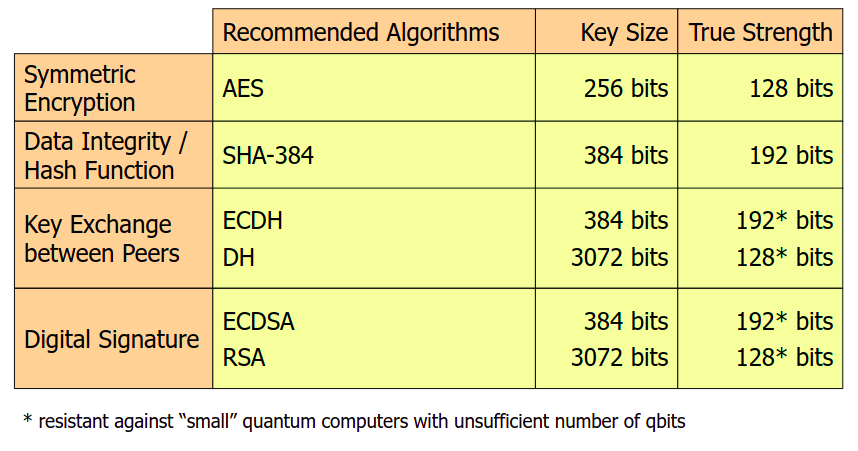
\includegraphics[width=0.8\linewidth]{images/cnsa-standard.png}
\end{minipage}



\section{Verschlüsselungsverfahren}
\subsection{Speed}
Wird für die Verschlüsselung die Hardwarebeschleunigung AES-NI verwendet ist ein Performancegewinn von ca. Faktor 4 - 5 zu erkennen (zumindest auf den Rechnern im Security Labor).
\begin{table}[h]
	\centering
	\begin{tabu} to \linewidth {l l X}
		\toprule 
		Ranking & Verfahren & Bemerkung \\
		\midrule
		1 & AES-GCM & \\
		2 & AES & Je kleiner die Schlüssellänge desto schneller. Je kleiner die Schlüssellänge desto weniger Runden (10, 12, 14) \\
		3 & Camellia & Konservativer gewählte Rundenanzahl (18, 24) \\
		4 & DES & \\
		5 & 3DES & 12-13 mal langsamer als AES-128 \\
		\bottomrule 
	\end{tabu} 
	\caption{Speed von Verschlüsselungsverfahren}
\end{table}

\subsection{Symmetrisch}
\subsubsection{AES: Advanced Encryption Standard}
\begin{itemize}
	\item Block Cipher mit einer Blockgrösse von 128 Bit
	\item Es gibt drei Varianten von Schlüssellängen, welche sich nur in den Anzahl Runden unterscheiden
	\begin{enumerate}
		\item 128Bit: 10Runden
		\item 192Bit: 12Runden
		\item 256Bit: 14Runden
	\end{enumerate}
	\item Neuere Intel CPUs unterstützen das \textit{aes-ni} (Hardwarebeschleunigung) Instruktionsset, welches den Algorithmus um Faktor zwei bis drei schneller macht. Dieser Modus ist standardmässig aktiviert.
	\item AES GCM ermöglicht eine Verschlüsselung des Plaintextes und garantiert die Integrität des generierten Ciphertextes, sowie zusätzlicher unverschlüsselter Daten durch eine kryptographische Checksumme. AES GCM hat einen hohen Datendurchsatz, weshalb dieser Modus gerne bei TLS Zertifikaten an den Anfang der Liste gesetzt wird.  Einerseits können alle Counter-Blöcke vorberechnet werden, sobald der IV und die Plaintext-Länge bekannt sind. Andererseits kann die Authentisierung von Ciphertext-Blöcken und die Verschlüsselung von weiteren Plaintext-Blöcken parallel ablaufen.
	\item Der Rechenaufwand ist (praktisch) proportional zur Anzahl der Runden
\end{itemize}

\paragraph{AES CTR: Counter Mode}
Der Counter Mode ist eine Betriebsart, in der Blockchiffren wie AES betrieben werden können, um daraus eine Stromchiffren zu erzeugen. Zur Verschlüsselung wird ein Initialisierungsvektor mit dem Schlüssel verschlüsselt und so ein Zwischenschlüssel produziert. Dieser wird im Anschluss mittels einer XOR-Operation mit dem Klartext kombiniert. Daraus entsteht der Geheimtext.



\subsubsection{Camellia}
Camellia verwendet die gleichen Parameter wie AES: eine Blockgröße von 128 Bit und Schlüssellängen von 128, 192 oder 256 Bit. Camellia wurde in Japan entwickelt und kann mit AES verglichen werden. Im Zweifelsfall sollte aber AES verwendet werden, da dieses Verfahren weiter verbreitet ist, und die Hardware eher für AES optimiert ist. Wie auch bei AES ist der Rechenaufwand, also die Performance, praktisch proportional zu der Anzahl der Runden.
\begin{itemize}
	\item Block Cipher mit einer Blockgrösse von 128 Bit
	\item Es gibt drei Varianten von Schlüssellängen, welche sich nur in den Anzahl Runden unterscheiden
	\begin{enumerate}
		\item 128Bit: 18Runden
		\item 192Bit: 24Runden
		\item 256Bit: 24Runden
	\end{enumerate}
\end{itemize}

Ebenfalls haben wir in den Übungen festgestellt, dass Camellia einiges langsamer ist als AES. Dafür gibt es folgende Gründe:
\begin{itemize}
    \item Die konservativer gewählte Rundenanzahl (AES: 10, 12, 14 Runden vs. Camellia: 18, 24, 24)
    \item Keine 64-bit Architektur Optimierung für die OpenSSL-Implementation
\end{itemize}

\subsection{AEAD}
AEAD steht für Authenticated Encryption with Associated Data und bezeichnet eine spezielle Klasse von Modi in welchen Blockciphers betrieben werden können, welche es erlauben Daten zu verschlüsseln und diese und weitere Daten (das AD in AEAD) gleichzeitig zu authentisieren. Ein Beispiel dafür ist der sogenannte GCM Modus (Galois/Counter Mode). Klassischerweise wurde zur Authentisierung von Nachrichten ein Message Authentication Code (MAC) verwendet. Häufig ist dies ein HMAC, welcher auf einer bestehenden Hash-Funktion basiert. 

\subsection{Asymmetrisch}
\subsubsection{RSA}
\textit{rsa} ist ein asymmetrisches kryptographisches Verfahren, das sowohl zum Verschlüsseln als auch zum digitalen Signieren verwendet werden kann.
\begin{itemize}
	\item RSA Signatur Schlüssel haben üblicherweise einen sehr kleinen öffentlichen Exponenten, bei dem nur zwei Bits auf 1 gesetzt sind. Im Gegensatz dazu ist das Modul und der private Exponent sehr gross, bei welchen etwa die Hälfte der Bits auf 1 gesetzt sind. Daraus resultiert, dass die Verifikation der Signatur sehr viel einfacher und schneller geht, wie die Generierung.
\end{itemize}

\paragraph{Vorgehen}
\begin{enumerate}
	\item Zwei Primzahlen wählen und Produkt bilden: $n = p \cdot q$
	\item $\varphi(n) = (p - 1) \cdot (q - 1)$
	\item Beliebige Zahl a wählen, wobei a teilerfremd zu $\varphi(n)$ sein muss. ($ggt(\varphi(n), a) = 1$) \\ $\Rightarrow$ am besten eignen sich Primzahlen für a. (privater Schlüssel)
	\item Multiplikative Inverse b berechnen (öffentlicher Schlüssel) $a \cdot b = 1$ mod $\varphi(n)$ $\Rightarrow$ erweiterter Euklidischer Algorithmus
	\begin{enumerate}
		\item Modul: n (öffentlich)
		\item Öffentlicher Schlüssel: b
		\item Privater Schlüssel: a
	\end{enumerate}	
\end{enumerate}

\paragraph{Verschlüsseln}
\begin{enumerate}
	\item $\text{Wert}_\text{verschlüsselt} = (\text{Wert}_\text{unverschlüsselt})^{b} \cdot mod(n)$
\end{enumerate}

\paragraph{Entschlüsseln}
\begin{enumerate}
	\item $\text{Wert}_\text{unverschlüsselt} = (\text{Wert}_\text{verschlüsselt})^{a} \cdot mod(n)$
\end{enumerate}

\subsubsection{DH: Diffie-Hellman}
DH ist ein asymmetrisches Verfahren, welches dazu verwendet wird einen symmetrischen Key zu generieren. Die Idee 
hinter diesem Verfahren ist, dass die beiden Partner gemeinsam den geheimen Schlüssel generieren (Shared Master Secret), ohne ihn 
ganz übermitteln zu müssen.

\paragraph{Vorgehen}
\begin{enumerate}
	\item One Way Function: $f(x) = g^x \text{ mod p}$
	\item Die Zahlen g und p sind öffentlich und können ungeschützt übertragen werden
	\item Alice und Bob einigen sich auf die Zahlen p und g
	\item Alice wählt eine zufällige Zahl a und sendet Bob den berechneten Wert gross A. $ A = g^a { mod(p)}$
	\item Bob wählt eine zufällige Zahl b und sendet Alice den berechneten Wert gross B. $ B = g^{b}{ mod(p)} $
	\item Beide können nun den geheimen symmetrischen Schlüssel K berechnen: $K= A^{b}{ mod(p)} $ rsp. $K= B^{a}{ mod(p)} $
\end{enumerate}


\section{Hashverfahren}
\subsection{Speed}
Auf 64Bit Plattformen ist SHA-2 512 schneller wie die SHA-2 256 Variante, da sie intern 64 Bit Wörter verwendet und die 256 nur 32Bit Wörter
\begin{table}[h]
	\centering
	\begin{tabu} to \linewidth {c l}
		\toprule 
		Ranking & Verfahren \\
		\midrule
		1 & MD5 \\
		2 & SHA-1 \\
		3 & SHA-2 \\
		4 & SHA-3 \\
		\bottomrule 
	\end{tabu} 
	\caption{Speed von Hashverfahren}
\end{table}

\subsection{MD5}
MD5 (Message Digest \#5) berechnet einen 128Bit langen Hash Wert. Er darf heutzutage nicht mehr verwendet werden, da er offiziell als gebrochen gilt. (seit 2013)

\subsection{SHA-1 }
SHA-1 (Secure Hash Algorithm) berechnet einen 160Bits langen Hash Wert. NIST empfiehlt seit 2005 SHA-1 nicht mehr zu verwenden. 

\subsection{SHA-2}
Es existieren 4 SHA-2 Implementierungen (Secure Hash Algorithm Family) mit unterschiedlichen Hash Längen (SHA-224, SHA-256, SHA-384 und SHA-512). Die SHA-2 Variationen haben immer genau die halbe Schlüsselstärke (SHA-384 $\Rightarrow$ Schlüsselstärke = 192Bits). Obschon SHA-2 noch weit verbreitet ist, sollte man nicht mehr auf SHA-2 setzen.

\info{Performance der SHA-384-Methode }{Die Performance von SHA-384 ist gleich wie die der 512-Bit-Variante. Der Grund ist, dass die 384-Bit Variante ist einfach ein verkürzter 512-Bit Hash. Es wird also ein 512-Bit berechnet und dann abgeschnitten um einerseit bei der Übertragung etwas Bandbreite zu sparen und andererseits nicht den gesamten letzten State preiszugeben.
}

\subsection{SHA-3}
Es existieren 4 SHA-3 (Keccak) Implementierungen mit unterschiedlichen Hash Längen (SHA3-224, SHA3-256, SHA3-384 und SHA3-512). SHA-3 ist der Gewinner eines NIST Wettbewerbs und wurde 2015 standardisiert. Keccak basiert nicht mehr auf dem ursprünglichen SHA.


\section{Elliptic Curves}
\begin{itemize}
	\item Die Schlüsselstärke ist immer die Hälfte der angegeben Schlüssellänge. (z.B ECDH256 $\Rightarrow$ 128bit)
	\item ECDSA ist wesentlich schneller wie RSA, da kleinere Schlüssel verwendet werden können.
	\item Mit dem D-Wave sind 1000Qbits möglich, jedoch wird der Shor's Quantum Algorithm nicht erfüllt, da nicht richtige Quantenzustände verwendet werden.
\end{itemize}
\begin{minipage}[t]{1\textwidth}
\centering
	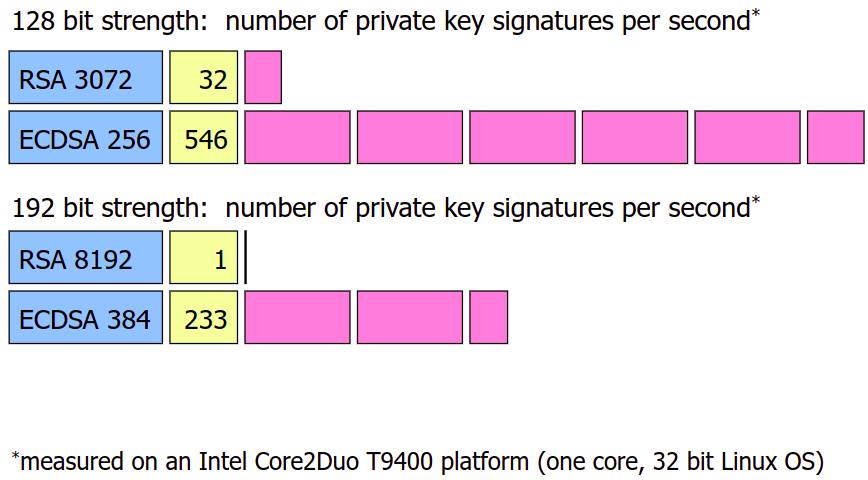
\includegraphics[width=0.6\linewidth]{images/rsa-vs-ecdsa.png}
\end{minipage}

\subsection{Kryptografische Stärke}
Die kryptografische Stärke des ECDH Algorithmus beruht darauf, dass es sehr aufwändig ist, die Anzahl Additionen eines Kurvenpunktes $P$ mit sich selber Modulo einer Primzahl $p$ (d.h., das $n$ in $nP \mod p = (P_1 + P_2 + ... + P_n) \mod p$) herauszufinden.

Grundsätzlich baut ECDH damit auf das gleiche bzw. ein sehr ähnliches Problem wie DH und RSA auf, allerdings ist ECDH gegen einige Angriffe resistent, welche die Faktorisierung von RSA/DH einfacher machen. Dadurch sind deutlich kürzere Schlüssel möglich.

\subsection{Gruppe}\label{sec:gruppe}
Eine Gruppe ist ein algebraisches System bestehend aus G und einer Operation *, sodass für alle Elemente a,b,c in G folgende Bedingungen gelten:
\begin{enumerate}
	\item a * b muss in G sein
	\item a * (b * c) = (a * b) * c
	\item Es gibt ein Neutrales Element $\Rightarrow$ a * e = e * a = a (z.B 0 bei einer Addition)
	\item Es gibt ein Inverses Element $\Rightarrow$ a * a' = a' * a = e (z.B a'=-a bei einer Addition)
	\item Man spricht von einer Abelschen Gruppe wenn gilt: a * b = b * a (Kommutativgesetz)
\end{enumerate}

\begin{figure}[ht!]
	\centering
	\begin{minipage}[t]{0.4\textwidth}
		\centering
		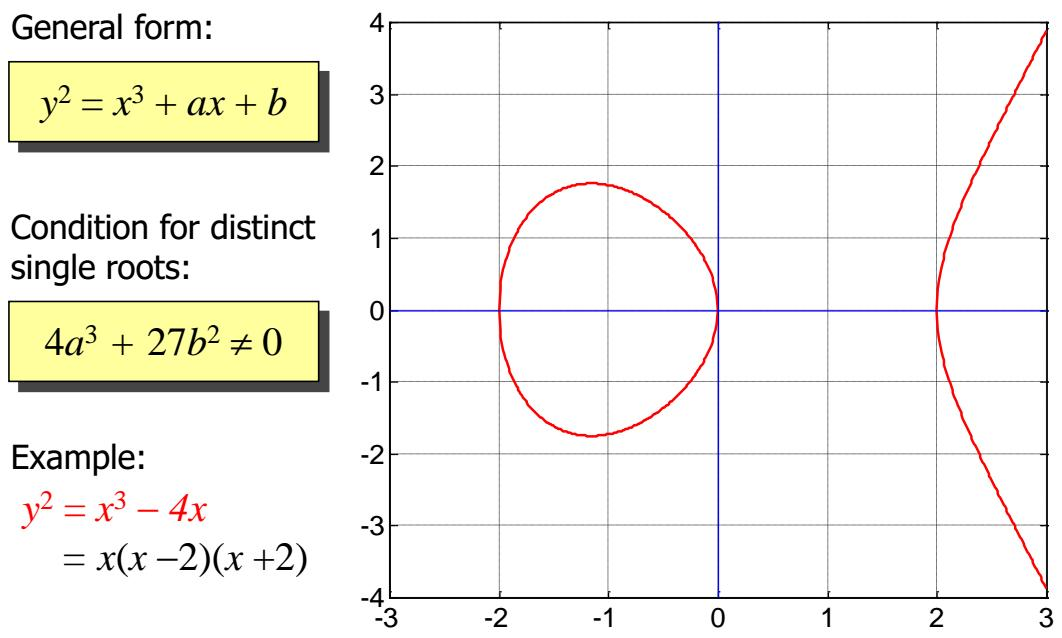
\includegraphics[width=\linewidth]{images/eliptic_curve_calculation}
		\caption{Elliptische Kurven Berechnung}
		\label{fig:elipticcurvecalculation}
	\end{minipage}
	\begin{minipage}[t]{0.4\textwidth}
		\centering
		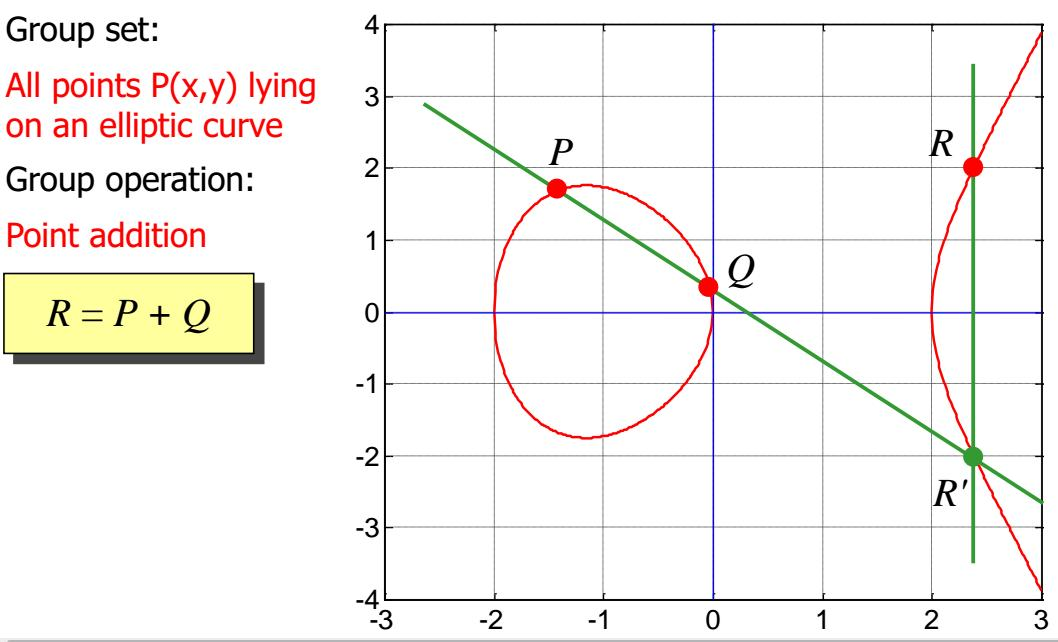
\includegraphics[width=\linewidth]{images/eliptic_curve_calculation2}
		\caption{Berechnung der Gruppe}
		\label{fig:elipticcurvecalculation2}
	\end{minipage}
\end{figure}

\begin{figure}[ht!]
	\centering
	\begin{minipage}[t]{0.4\textwidth}
		\centering
		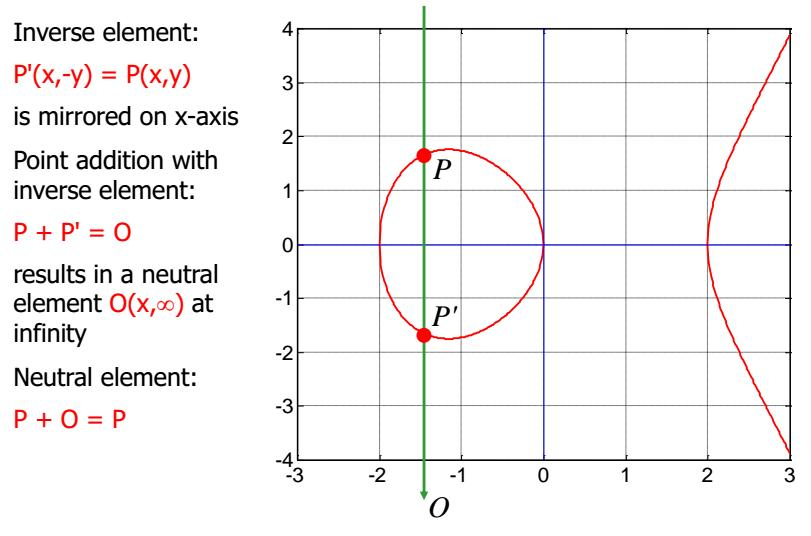
\includegraphics[width=\linewidth]{images/eliptic_curve_calculation_neutral_inverse_elem}
		\caption{Inverses und Neutrales Element}
		\label{fig:elipticcurvecalculationneutralinverseelem}
	\end{minipage}
	\begin{minipage}[t]{0.4\textwidth}
		\centering
		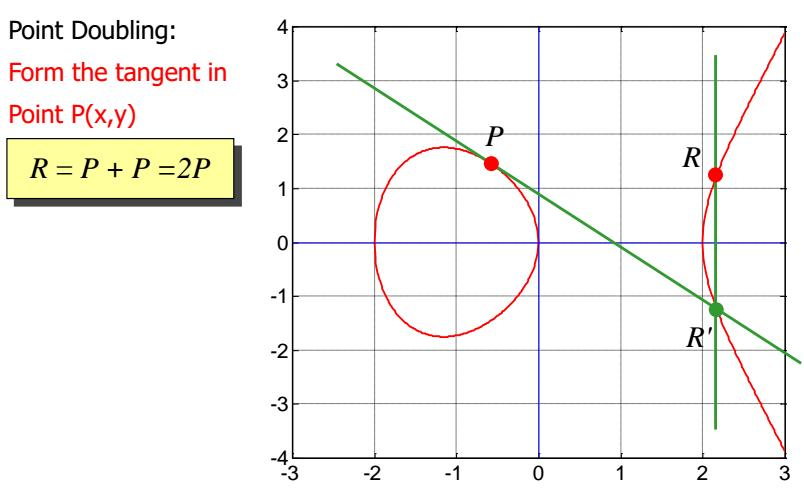
\includegraphics[width=\linewidth]{images/eliptic_curve_calculation_point_doubling}
		\caption{Q und P werden so verschoben, dass sie eine Tangente bildern}
		\label{fig:elipticcurvecalculationpointdoubling}
	\end{minipage}
\end{figure}

\begin{figure}[ht!]
	\centering
	\begin{minipage}[t]{0.4\textwidth}
		\centering
		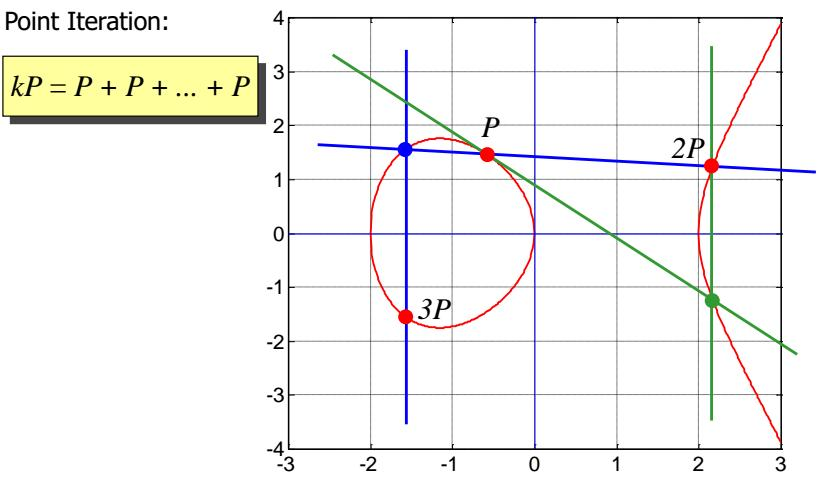
\includegraphics[width=\linewidth]{images/eliptic_curve_calculation_point_iteration}
		\caption{Point Iteration: Einen Punkt k-1 mal zu sich selbst hinzufügen}
		\label{fig:elipticcurvecalculationpointiteration}
	\end{minipage}
	\begin{minipage}[t]{0.4\textwidth}
		\centering
		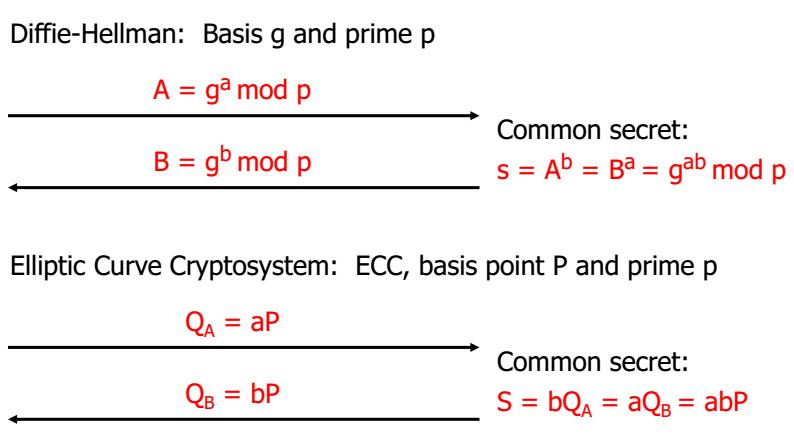
\includegraphics[width=\linewidth]{images/eliptic_curve_key_exchange}
		\caption{Schlüsselaustausch}
		\label{fig:elipticcurvekeyexchange}
	\end{minipage}
\end{figure}

\newpage
\subsection{ECDH}
Die Schwierigkeit bei ECDH ist es, die Anzahl Punktadditionen herauszufinden (privater Teil)

\begin{enumerate}
	\item Alice und Bob einigen sich auf eine Elliptische Kurve, einen Punkt auf der Kurve $P$ aus der Zahlengruppe $G$ (siehe Sektion \ref{sec:gruppe}). Diese werden ungeschützt übertragen.
	\item Alice wählt eine zufällige geheime Zahl $a$, Bob wählt eine zufällige geheime Zahl $b$
	\item Alice übermittelt Bob den ''Public Key'' $A = aP$, Bob übermittelt Alice seinen ''Public Key'' $B = bP$ über einen ''öffentlichen'' Kanal.
	\item Alice und Bob können nun mithilfe der vorhandenen Zahlen den gemeinsamen geheimen Schlüssel ausrechnen: $\text{ (Alice:) } aB = \text{ (Bob:) } bA = abP$.
\end{enumerate}

\subsection{Curve25519}
In der Kryptographie ist Curve25519 eine elliptische Kurve, die \textbf{128 Bit Sicherheit (kryptographische Stärke)} bietet und für die Verwendung mit dem elliptischen Diffie-Hellman (ECDH)-Schlüsselvereinbarungsschema entwickelt wurde. 
$y^2 = x^3 + 486662x^2 + x$ in einem endlichen Körper modulo der Primzahl $2^{255} - 19$


\subsection{Prüfungsaufgabe FS13}
\begin{minipage}[t]{1\textwidth}
    \centering
	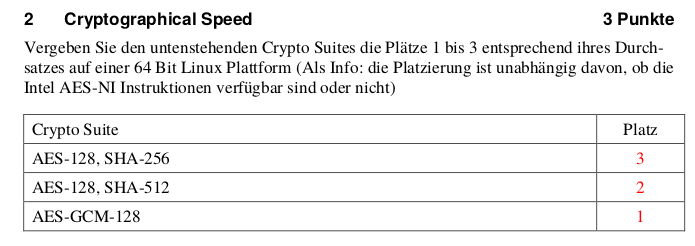
\includegraphics[width=0.9\linewidth]{images/fs13-crypto-speed.png}
    \caption{}
    \label{fig:keystrenghtcomparison}
\end{minipage}


\section{Physical Layer Security}
Auf dem Physical Layer gibt es nur Quanten Kryptographie das kryptographisch sicher ist.

\paragraph{Frequency Hopping}\hfill
\\
Zusätzlich gibt es noch Frequency Hopping: Bei diesem Verfahren wird das Frequenz Band in verschiedene Kanäle eingeteilt. Zwischen diesen Kanälen wird dann hin und her gewechselt. Viele kabellose Kommunikationsstandards und -geräte benutzen dieses Verfahren für die Übertragung (dass das Signal wegen Überlagerungen nicht ausgelöscht wird). Bei diesen Verfahren ist die Hoppin-Sequenz bekannt.

Bei anderen Systemen legt ein geheimer Schlüssel (PRF oder Rückgekoppeltes Schieberegister)  die Reihenfolge fest. Kann man das ganze Frequenzspektrum überwachen, so kann die Reihenfolge der Kanäle erahnt werden. Obwohl das Verfahren nicht (mehr) sicher ist, wird es noch immer in der Schweizer Armee für die Funkgeräte eingesetzt. Dort wird das Verfahren \grqq security by obscurity\grqq immer noch grossgeschrieben.

\subsection{Quanten Kryptographie - Quantum Key Distribution}
Bei der Quanten Kryptographie, oder besser gesagt Quantenschlüsselaustausch, nutzt man die Eigenschaften der Quantenmechanik, damit zwei Parteien eine gemeinsame Zufallszahl generieren können, die als geheimer Schlüssel verwendet werden kann. Dieser geheime Schlüssel kann dann für die (symmetrische) Verschlüsselung verwendet werden. Der Austausch eines geheimen Schlüssels mit Hilfe der Quantenmechanik gilt als absolut sicher. Einerseits, weil das Abhören mit Sicherheit bemerkt wird. Andererseits, weil die Schlüsselverteilung auf bekannten physikalischen Gesetzmässigkeiten beruhen und nicht mit Rechenleistung geknackt werden kann. 
\\
Grundsätzlich gibt es zwei verschiedene Verfahren:
\begin{enumerate}
    \item Verschränkte (entangled) Photonen - wird beim E91 Protokoll verwendet 
    \item Photonen als Übertragung - wird beim BB84 Protokoll verwendet
\end{enumerate}

\subsubsection{Verschiedene Polarisationen}
Jedes Photon kann genau eine von vier möglichen 45 Grad Polarisationen ($0^{\circ},45^{\circ},90^{\circ},135^{\circ}$)).) annehmen:
\begin{itemize}
    \item Horizontal (-)
    \item Vertikal (|)
    \item Linksdiagonal (\textbackslash)
    \item Rechtsdiagonal (/)
\end{itemize}
Diese Polarisationen (und andere Photoneneigenschaften) sind schlussendlich der Grund, wieso dieses Verfahren absolut sicher ist. 

\subsubsection{Verschränkte (entangled) Quanten}
Bei dieser Methode werden sogenannte verschränkte Quanten verwendet. Eine Photonen Quelle erstellt für jedes mögliches Schlüsselbit ein verschränktes Photonenpaar. Diese Zwillings Photonen weisen die komplementäre Polarisationen auf und sind daher eindeutig identifizierbar. Versucht nun ein Angreifer mitzulesen, so wird die Polarisation verändert, dies wird aber erkannt, da sich beide Kommunikationspartner über die verwendeten Phtotonen austauschen. Das Duplizieren eines Photons wird  ebenfalls bemerkt, da das ganze System zerstört wird und das neue Photon nicht mehr zu seinem Zwilling passt.



\subsubsection{Ekert E91 Protokoll}
Laser erzeugt für jedes mögliche Schlüsselbit ein verstränktes (entangled) Photonenpaar. Eines erhaltet der Sender (Alice) das andere der Empfänger (Bob). Beide Kommunkationspartner wählen bei jedem erhaltenen Bit rein zufällig eine Filter-Einstellungen (50/50). Diese Einstellung definiert, ob eine vertikale/horizontale oder eine diagonale Messung (um $45^{\circ}$ verschoben) verwendet wird. Nachdem sie eine Reihe von verschränkten Photonen empfangen haben, teilen sie sich gegenseitig mit, welche Filtereigenschaft sie bei welchem Bit verwendet haben. Bei 50\% der Übertragungen haben sie  die gleichen Einstellungen verwendet, diese Bits werden nun für den Schlüssel verwendet. Alle Messwerte mit den falschen Einstellungen werden verworfen. Somit werden automatisch alle Messungen verworfen, wo ein Angreifer (z.B Eve) mitgelauscht hat, da die Phototeneigenschaften falsch waren.\\
Wenn mehrere Photonen nicht ankommen (einzelne können von der Glasfaser geschluckt werden), kann der Empfänger davon ausgehen, dass die Leitung abgehört wird. Das Protokoll funktioniert aber nur auf Distanzen bis ca. 10km.

\begin{minipage}[t]{1\textwidth}
    \centering
	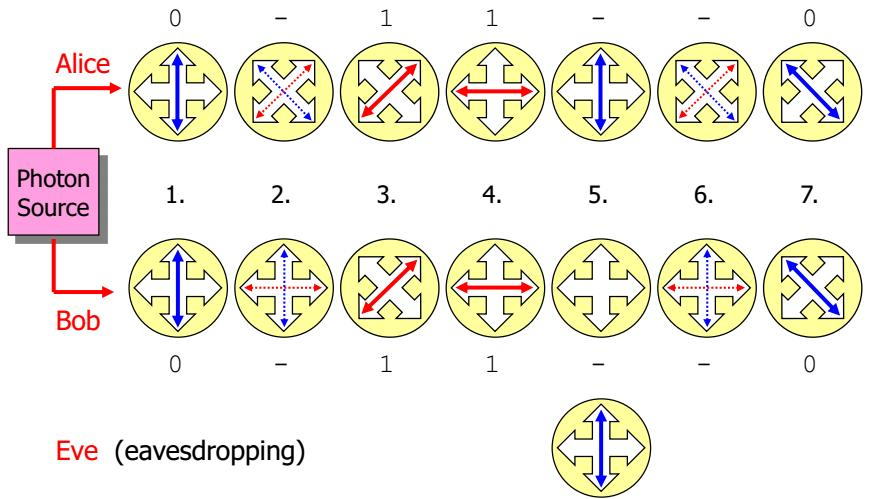
\includegraphics[width=0.9\linewidth]{images/entangled_photons}
    \caption{}
\label{fig:entangledphotons}
\end{minipage}


\subsubsection{BB84 Protokoll}
Beim BB84 braucht man keine verschränkte Photonen Paare. Hier wird nur ein einzelnes polarisierte Photon versendet, welches eine der 4 Zustände (Polarisationen) annehmen kann. Mit diesem Verfahren können Distanzen von 50-150km überwunden werden.

\begin{minipage}[t]{1\textwidth}
    \centering
	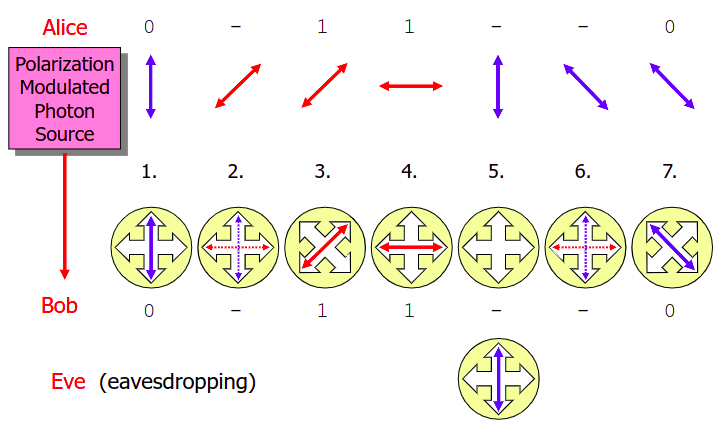
\includegraphics[width=0.9\linewidth]{images/bb84.png}
\label{fig:entangledphotons}
\end{minipage}

\paragraph{Ablauf}
Die Polarisation jedes empfangnen Photons wird von Bob mit einem zufällig gewählten Filterset gemessen (Rectilinear oder Diagonal). Nach den erfolgten Messungen gibt Bob über einen unsicheren 
Kanal bekannt, welches Filterset er jeweils für die Polarisationsbestimmung jedes Photons verwendet hat. Alice gibt anschliessend für jedes gesendete Photon bekannt, ob es rectilinear oder diagonal polarisiert wurde und ob es sich um einen Decoy-Puls oder einen normalen Puls gehandelt hat. 

\info{Decoy Pulse}{Decoy Pulse sind Fake Protonen, welche vom Sender vereinzelt mitgesendet werden. Ist die Übertragung beendet meldet der Sender dem Empfänger, welches Decoy Pulse gewesen sind. Unterscheidet sich die Zahlen der Decoy Statistik, so weiss man, dass ein Angreifer mitgehört hat.  }

\paragraph{Sicherheit}
Beide Kommunikationspartner (Alice \& Bob) vergleichen eine bestimmte Untermenge ihrer Bitfolgen miteinander. Hat ein Angreifer (Eve) Informationen über die Polarisation der Photonen gewonnen, so führt dies zu Fehlern bei Messungen vom Empfänger (Bob). Diese Fehler werden dann erkannt. Gibt es zu viele Fehler wird das Verfahren abgebrochen und neugestartet.

\paragraph{Decoy States}
Um zu verschleiern, dass Photonen gestohlen wurden, könnte ein Angreifer bewusst Decoy States einfügen. Als Gegenmassnahme fügt der Sender zufällige Decoy States ein und sagt dem Empfänger welches die Decoy States waren. Die Decoy States werden auf einem niedrigeren Leitungspegel ausgesendet. Wenn der Angreifer auf der Leitung sitzt, resultiert eine andere statistische Verteilung (von Daten und Decoy Pulsen), was wiederum erkannt werden kann.


\paragraph{Verlust}
Je grösser die Übertragungsdistanz  ist, desto mehr nehmen die Bit Slots ohne Information zu. Bei einer 1550nm breiten Fiber hat man Dämpfung von 0.2dB/km. Daraus resultieren folgende Verluste:
\begin{itemize}
	\item 50km: 10dB $\rightarrow$ 1 von 10 Photonen überlebt
	\item 100km: 20dB $\rightarrow$ 1 von 100 Photonen überlebt
	\item 150km: 30dB $\rightarrow$ 1 von 1000 Photonen überlebt
\end{itemize}

\subsubsection{Shor's Quantum Algorithm}
Für eine Zahl $n$ benötigt man einen Quantencomputer mit $\log(n)$ Qubits. 

\subsubsection{Grovers's Quantum Algorithm}
Der Grover-Algorithmus beweist, dass Quantencomputer prinzipiell schneller als klassische Computer sind. 

\subsubsection{No-Cloning-Theorem}
Das No-Cloning-Theorem besagt, dass es nicht möglichist , ein System zu bauen, das jedes beliebige Qubit perfekt auf ein anderes Qubit kopiert, ohne dabei das ursprüngliche zu verändern. Es ist einer der Gründe, wieso der Quantenschlüsselaustausch so sicher ist.

\subsubsection{Quantenresistente Algorithmen}
Für \textbf{AES} wurde nachgewiesen, dass der Einsatz von Quantencomputer die \textbf{Schlüssellänge halbiert}. Eine einfache Lösung für das Problem ist deshalb, dass man einfach doppelt so grosse Schlüssellängen verwendet. 
\begin{description}
	\item[New Hope] Gitterbasierter Post-Quanten Algorithmus (Wird von Google z.Z. mit TLS in Kombination mit Curve25519 getestet.)
\end{description}

\subsubsection{Prüfungsaufgaben}
\paragraph{BB84 Protkoll} \hfill
\newline
\begin{minipage}[t]{1\textwidth}
    \centering
	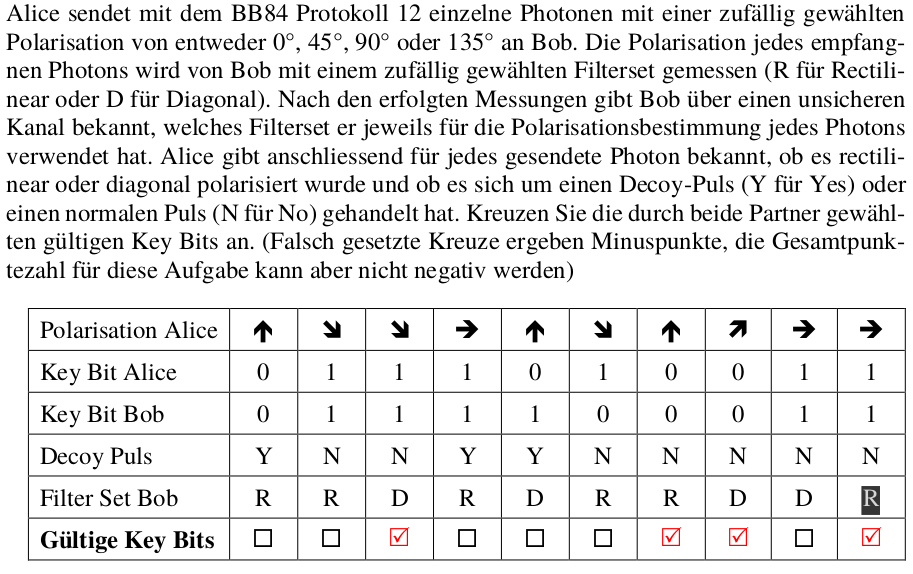
\includegraphics[width=0.9\linewidth]{images/hs18-19-bb84.png}
\end{minipage}
\paragraph{Dämpfung} \hfill
\newline
\begin{minipage}[t]{1\textwidth}
    \centering
	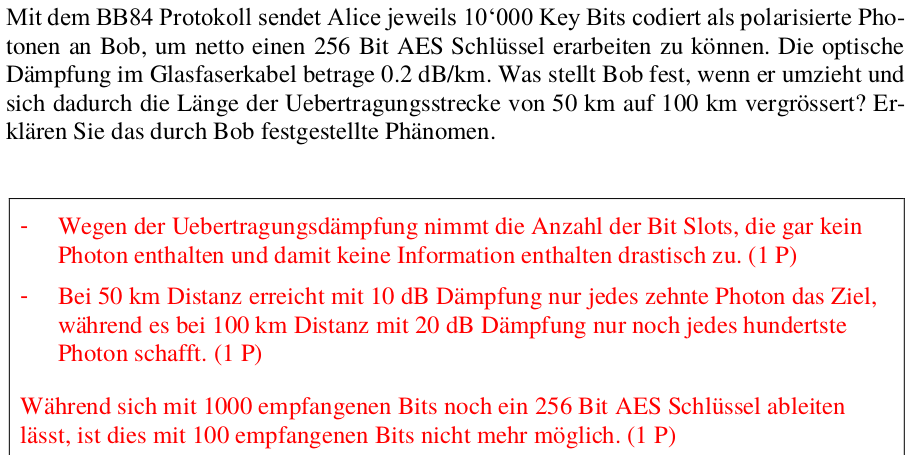
\includegraphics[width=0.9\linewidth]{images/hs18-19-daempfung.png}
\end{minipage}


\section{Zufallszahlen}
Je länger eine Zufallszahl verwendet wird (z.B mehrere Jahre) , desto besser sollte die verwendete Zufallsquelle sein. Eine gute Zufallsquelle liefert stetig Zufallszahlen, die einer guten statistischen Verteilung unterliegen.

\subsection{Eigenschaften}
Gute PRF (Pseudo Random Function) haben folgende Eigenschaften
\begin{itemize}
	\item Liefert ständig und zuverlässig (ohne Unterbrüche) Zufallsinformationen
	\item Hat keine Tendez (Bias) zu 0 oder 1, d.h. hat eine gute statistische Verteilung.
\end{itemize}

\subsection{PRF: Pseudo Random Functions}
Ein PRF nutzt eine echte Zufallsquelle als Seed und füttert damit einen Algorithmus. 

\subsubsection{HMAC Functions}
Der Schlüssel und der Seed wird aus einer echten zufälligen Quelle bezogen (z.B Quantenquelle) Der Seed wird mit dem Key der HMAC-Funktion übergeben. Dies wird dann solange wiederholt, bis man genügend Bytes Entropie hat. TLS nutzt HMAC PRF für Key Derivation.

\begin{figure}[h]
\centering
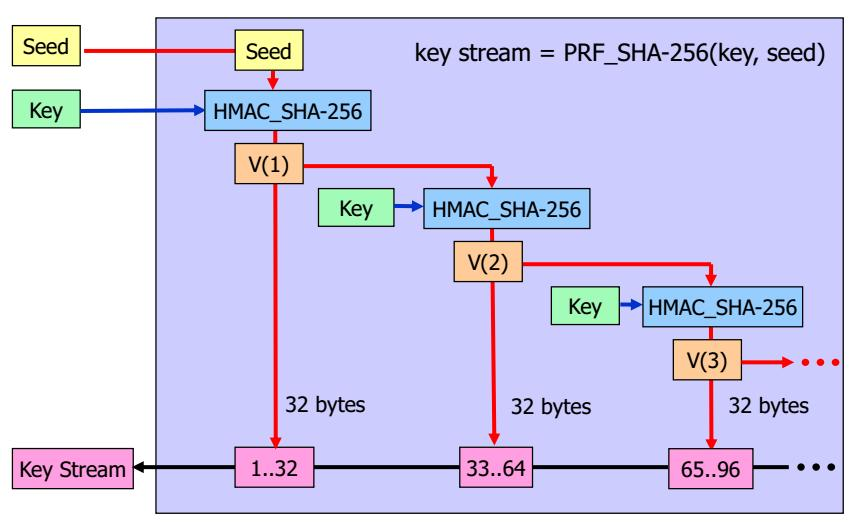
\includegraphics[width=0.7\linewidth]{images/hmac_prf}
\caption{HMAC PRF}
\label{fig:hmacprf}
\end{figure}


\subsubsection{DRBG: Deterministic Random Bit Generator}
Möchte man einen Key mit einer Schlüsselstärke ''X'' generieren, muss ein DRBG mindestens ''X'' Bits \textbf{Entropy Input} + $\frac{X}{2}$ Bits für die Random Nonce. Ein DRBG hat mehrere Inputs:


\begin{description}
	\item[Seed]	Das ''Kaffeepulver'' aus eineren wahren Zufallsquelle
	\item[Instantiate] Wie Stark soll die Sicherheit sein: (112Bit), (128Bit), 192Bit, 256Bit
	\item[Entropy Input] Entropy with size at least equal to security strength
	\item[Nonce] \hfill 
	\begin{itemize} 
		\item Entropy with size at least equal to 0.5 * security strength
		\item Counter with repetition rate at least equal to 0.5 * security strength
	\end{itemize}
	\item[Personalization String]  \hfill \\
	Application Identifiers, Device Serial Numbers, User IDs, etc. (Optional, can be an empty string)
	\item[Additional Input] Any other private or public input (Optional, can be empty)
\end{description}
\begin{figure}[h]
\centering
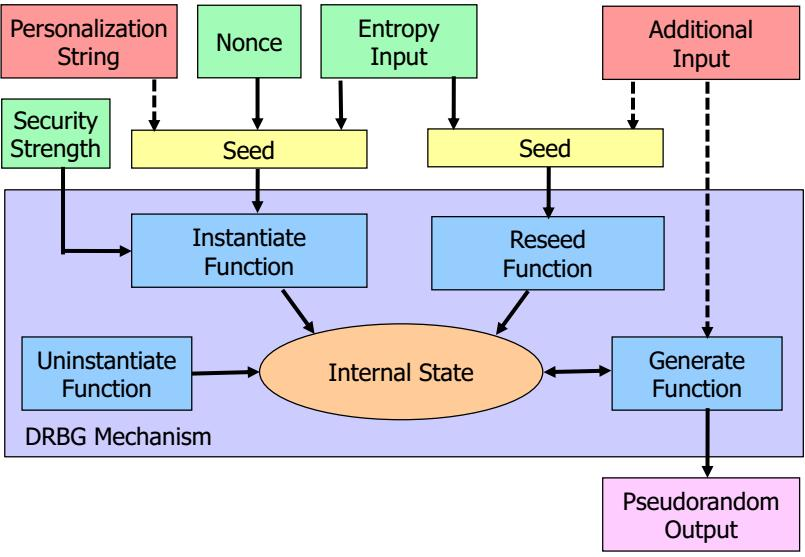
\includegraphics[width=0.5\linewidth]{images/drbg}
\caption{DRBG}
\label{fig:drbg}
\end{figure}

\subsection{Echte Random Generatoren}
Bei echten Random Generatoren (True Random Number Generators) zieht man die zufälligen Zahlen meist aus physikalischen Prozessen. Am besten ist, wenn man mehrere Quellen miteinander kombiniert.
\begin{itemize}
	\item Quantenquellen (die beste Quelle)
	\item Thermisches Rauschen 
	\item Radioaktiver Zerfall
	\item Intel RDRAND (gut und sehr schnell, sollte mit anderen Quellen vermischt werden, da evtl. die NSA ihre Finger im Spiel hat)
	\item Key Stroke Timing - Zeit zwischen Tastenbetätigungen (kleine Entropie)
	\item Mouse Movements Coordinates (grosse Entropie)
	\item Soundcard Input Noise (Gefahr von Gesamtausfall)
	\item Air Turbulence in Disk Drives (Veraltet, da SSD)
	\item Network Packet Arrival Times (eher verpönt, da manipulierbar)
\end{itemize}


\section{Data Link Layer Security}

\subsection{IEEE 802.1X Access Control using EAP Methods}
Der Client (Supplicant) stellt eine Anfrage über eapol (Extensible Authentication Protocol over Local Area Network) an eine Access Point oder LAN Switch (Authenticator). Dieser leitet die Anfrage an einen Radius Server (Authentication Server) über EAP RADIUS weiter. Der RADIUS-Server überprüft dann, ob die Authentifizeriung valide ist und sendet die Antwort zurück.

\subsection{Secure Device Identity (IEEE 802.1AR - DevID)}
\paragraph{Grundlagen}
Während der Herstellung wird eine IDevID (Initial Device Identifier) sowie ein X509 Zertifikat direkt auf die Hardware (DevID Module) geschrieben. Das DevID Modul verfügt zusätzlich über einen starken \textit{rng} (Random Number Generator) und implementiert starke asymmetrische Algorithmen (2048 RSA oder 256 ECDSA) sowie eine Hash Funktion (SHA-256). Auf dem DevID Module kann eine LDevID (Local Significant Device Identifier) hinterlegt werden. \\

Es gibt bis anhin sehr wenige Geräte, welchen diesen Standard unterstützen/implementieren.

\paragraph{Übersicht} \hfill
\newline
\begin{minipage}[t]{1\textwidth}
    \centering
	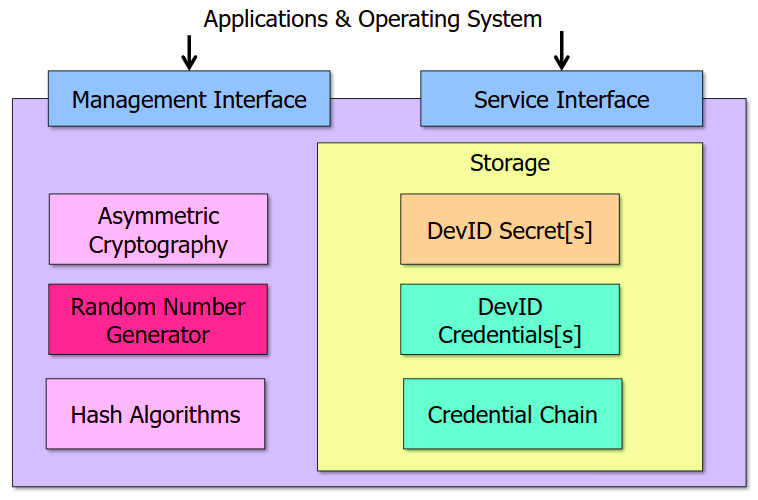
\includegraphics[width=0.7\linewidth]{images/devID-module.png}
\end{minipage}

\paragraph{Verwendung}
DevIDs könne für folgende Zwecke verwendet werden:
\begin{itemize}
    \item Geräteauthentifizierung mit DevID-Zertifikat (z.B EAP-TLS-Authentifizierung)
    \item Verwendung von DevIDs bei Geräten
    \begin{itemize}
        \item Switch, Router, AP oder AAA-Server((Authentication, Authorization, and Accounting) überprüft valide Werte im DevID Zertifikat
        \item Sicherer als MAC-Adressliste (MAC kann einfach gefälscht werden)
    \end{itemize}
\end{itemize}

\subsection{MACsec: Media Access Layer Security (IEEE 802.1AE)}\label{sec:macsec-media-access-layer-security-ieee-8021ae}
MACsec erlaubt \textbf{sichere E2E Verbindungen} über Ethernet zwischen direkt verbunden Clients. MACsec nutzt \textbf{AES-GCM-128} für die Verschlüsselung. Seit 2011 kann auch AES-GCM-256 verwendet werden. Eine neuer PAE muss den pre-shared CAK des CA-Verbund kennen
\begin{description}
	\item[PAE: Port Access Entity] Ein Client (SecY - MAC Security Entity). Jede PAE hat einen Secure Channel zu allen anderen Mitglieder in der CA. Jeder PAE muss den CAK der CA besitzen. 
	\item[CA: Connectivity Association] Verbund von mehrere Clients auf L2 mit einem gemeinsamen Netzwerkschlüssel
	\item[CAK: Connectivity Association Key] Statischer Schlüssel die jede PAE/SecY in der CA kennen muss. Diese müssen manuell verteilt werden. (Im Heim-WLAN auch als \textit{psk} bezeichnet.) Der CAK verschlüsselt die Control Plane. Der CAK ist somit das Shared Secred eines CA Verbund.
	\item[CKN: CAK Name] Netzwerk Identifier (am besten Human-Readable; WLAN: SSID)
	\item[SAK: SA Key] Secure Association Key (Session Key). Es wird für jeden Client ein SAK benötigt. Jeder SAK wird vom CAK abgeleitet. (Hash über den CAK OR-verknüpft mit einem Random Wert des Key Servers). Der Keyserver ist entweder ein PAE oder der Access Point. Der SAK verschlüsselt die Data Plane.
	\item[SC: Secure Channel] Jede SC umfasst eine Reihe von SA mit unterschiedlichen SAK's. Jeder SC ist unidirectional. 
	\item[SA: Secure Association] Eine Verbindung zwischen zwei Clients. Es gibt mehrere SA's innerhalb einer SC. Jede SA hat seinen eigenen SAK. Es dürfen mehrere Associations innerhalb von einem SA in eine Richtung koexistieren, damit die SAK's (der SA) unterbruchsfrei ausgetauscht werden können.  Die SA's haben dann nur eine begrenzte Lebensdauer, während die SC's als Grundelemente einer CA immer existieren. 
\end{description}

\begin{figure}[ht!]
	\centering
	\begin{minipage}[t]{0.4\textwidth}
		\centering
		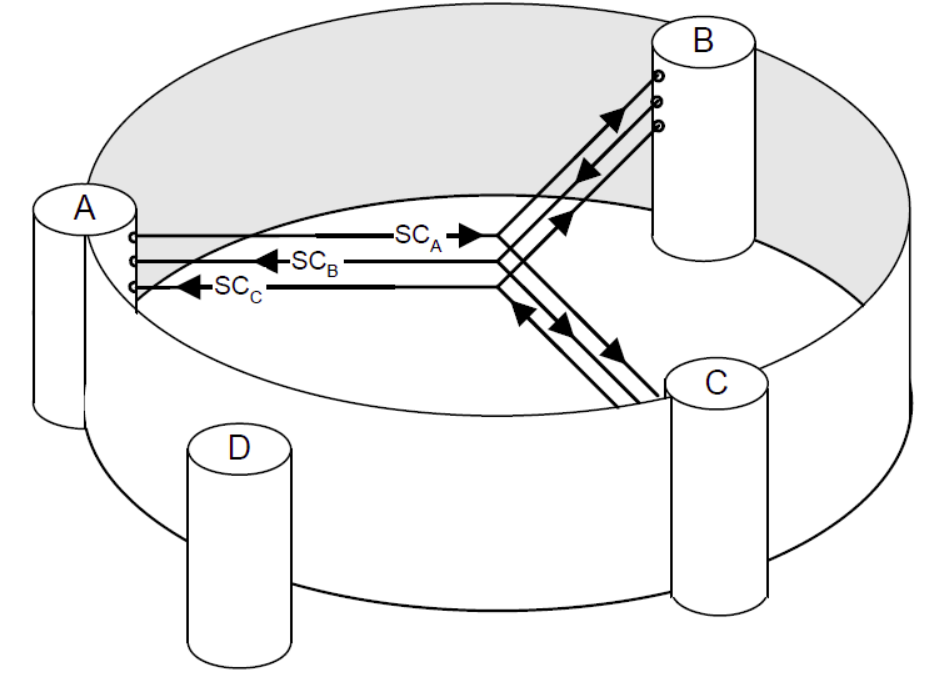
\includegraphics[width=0.9\linewidth]{images/macsec-overview-sc.png}
		\caption{Mehrere Stationen}
	\end{minipage}
	\begin{minipage}[t]{0.4\textwidth}
		\centering
		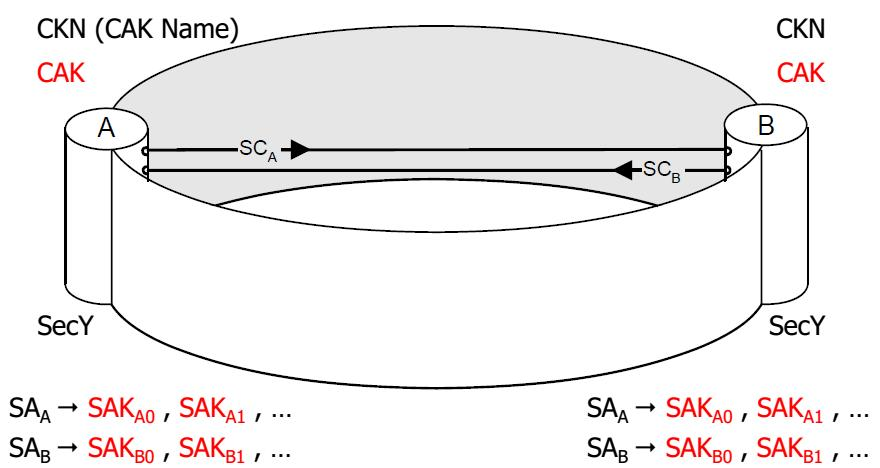
\includegraphics[width=0.9\linewidth]{images/macsec_sc_sa}
		\caption{Point-to-Point}
	\end{minipage}
\end{figure}
\subsubsection{MKA: MACsec Key Agreement Protocol}
Dank dem 802.1X MACsec Key Agreement (MKA) Protokoll
können die SAK's mittels eines Key Servers dynamisch generiert und an alle Teilnehmer verteilt werden. Damit ist ein periodisches Rekeying möglich.

\subsubsection{SAI: Secure Association Identifier}
Der Secure Association Identifier dient als ID für eine SA. Er besteht aus einem System Identifier, einem Port Identifier und einer Association Number. Die 2 Bit lange Association Number erlaubt es, dass währende dem Rekeying zwei verschiedenen SAK's koexistieren können.
\begin{minipage}[t]{1\textwidth}
    \centering
	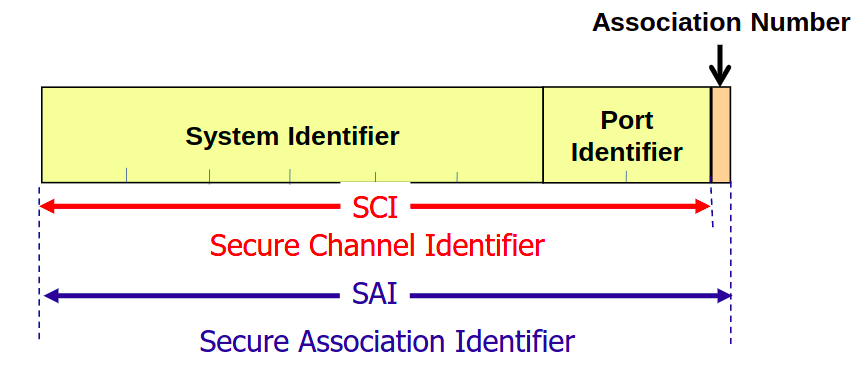
\includegraphics[width=0.7\linewidth]{images/macsec_sai.png}
\end{minipage}


\subsubsection{MACsec Frames}
\begin{minipage}[t]{1\textwidth}
    \centering
	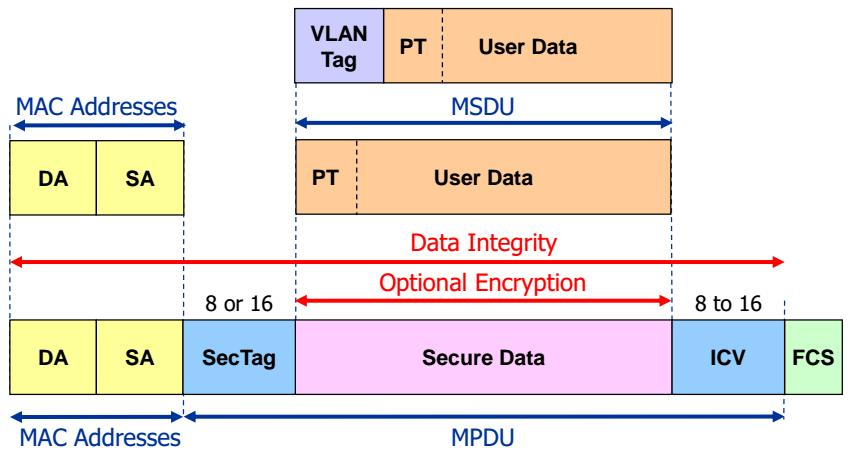
\includegraphics[width=0.7\linewidth]{images/macsec_frame_format}
\end{minipage}



\begin{description}
	\item[MPDU: MACsec Protocol Data Unit] Beinhaltet SecTag, Payload und ICV. Die PDU werden mit \textit{eapol} verteilt.
	\item[MSDU: MAC Service Data Unit] Payload
	\item[ICV: Integrity Check Value] Ist der Authentication Tag der aus AES GCM/AES GMAC resultiert.
	\item[SA, DA] Source und Destination MAC Adresse im Klartext
	\item[SecTag] Security Tag vor dem Payload  im Klatext
	\begin{itemize}
		\item MACsec Ethertype (Ethertype 0x88E5) (Das E Flag definiert ob verschlüsselt oder nur authentisiert)
		\item TCI – TAG Control Information (6 bits) 
		\item AN – Association Number (2 bits)
		\item SL – Short Length (6 bits) - gibt Anzahl Bytes von User Data an, falls die miinimale Ethernet Frame Grösse von 64 Byte nicht erreicht wird
		\item PN – Packet Number – replay protection and IV for encryption (4 bits)
		\item SCI – Secure Channel Identifier - dentifies Secure Association (SA). (0 - 8 bits)
	\end{itemize}
\begin{minipage}[t]{1\textwidth}
    \centering
	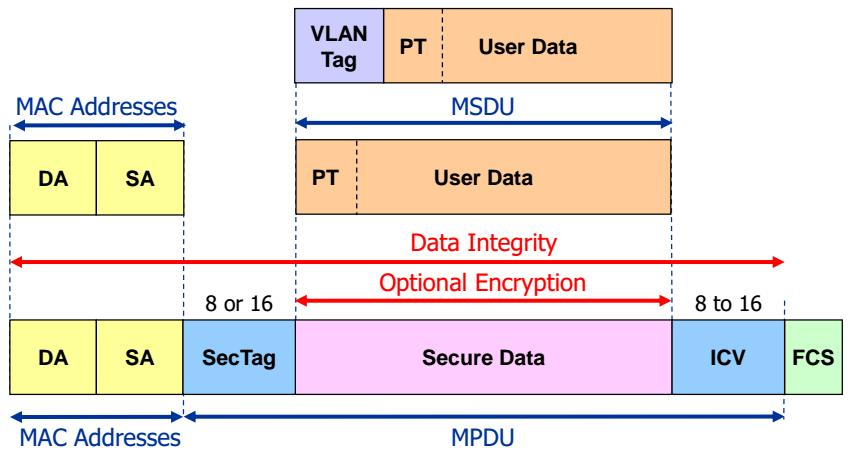
\includegraphics[width=0.6\linewidth]{images/macsec_frame_format}
\end{minipage}
	\item[FCS: Frame Check Sequence] 
\end{description}

\subsection{Prüfungsaufgaben}


\begin{minipage}[t]{1\textwidth}
    \centering
	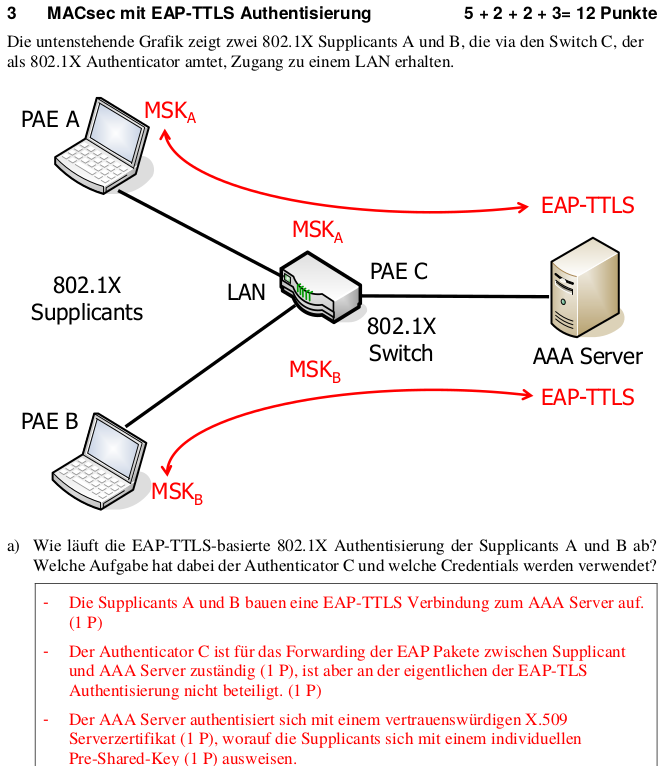
\includegraphics[width=0.9\linewidth]{images/hs18-19_macsec_exc1.png}
\end{minipage}

\begin{minipage}[t]{1\textwidth}
    \centering
	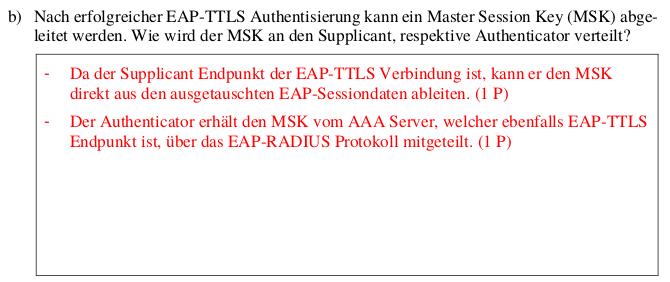
\includegraphics[width=0.9\linewidth]{images/hs18-19_macsec_exc2.png}
\end{minipage}

\begin{minipage}[t]{1\textwidth}
    \centering
	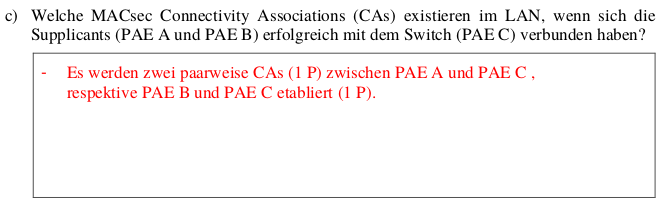
\includegraphics[width=0.9\linewidth]{images/hs18-19_macsec_exc3.png}
\end{minipage}

\begin{minipage}[t]{1\textwidth}
    \centering
	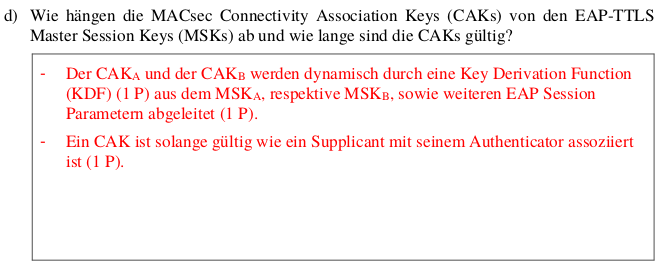
\includegraphics[width=0.9\linewidth]{images/hs18-19_macsec_exc4.png}
\end{minipage}

\begin{minipage}[t]{1\textwidth}
    \centering
	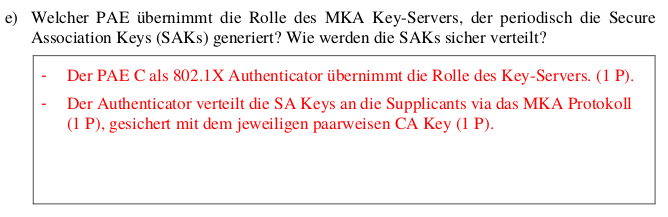
\includegraphics[width=0.9\linewidth]{images/hs18-19_macsec_exc5.png}
\end{minipage}


\section{VPN: Virtual Private Network}
Mittels VPN kann ein sogenannter Road Warrior (Client) von einem beliebigen Punkt auf der Erde via Internet auf sein heimatliches Firmennetz zugreifen. Bei IPsec geschieht das über einen verschlüsselten Tunnel, der zwischen Remote Access Client und dem Security Gateway des Heimatnetzes aufgebaut wird. Die Authentisierung der beiden Tunnelpunkte wird über ein X.509 Zertifikate bzw. Benutzername/Passwort bewerkstelligt. Es gibt verschiedene Varianten von VPNs wobei wir den Schwerpunkt auf IPsec legen. Aktuell wird IPsec mit IKEv2 empfohlen.

\subsection{Terminologie}
\begin{description}
 \item [PPP - Point-to-Point Protocol] Das Point-to-Point ist ein Layer 2 Protokoll und dient, wie der Name schon erraten lässt, dem Aufbau einer Point-to-Point Verbindung. Es ist möglich eine Authentifizierung (PAP. CHAP) oder eine Verschlüsselung (ECP) zu aktivieren.
 \begin{minipage}[t]{0.6\textwidth}
		\centering
		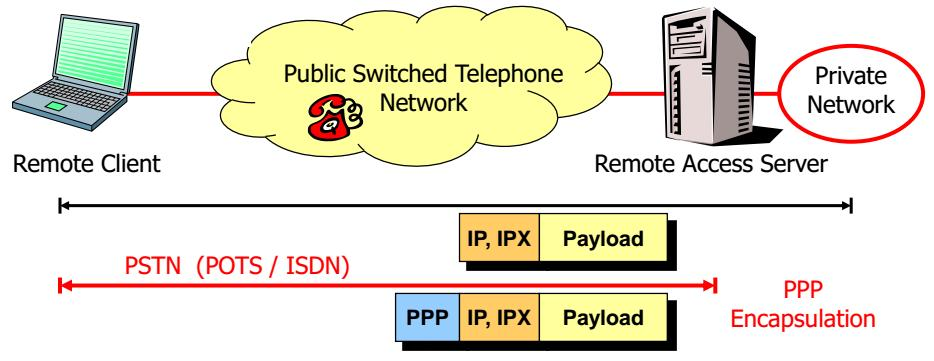
\includegraphics[width=\linewidth]{images/ppp_remote_access}
	\end{minipage}
	\item[VPN] Das konventionelle VPN bezeichnet einzig eine logische Trennung innerhalb einer physischen Leitung. Dabei wird zwischen verschiedenen VPNs unterschieden:
\begin{itemize}
        \item Layer 2 Tunneling Protocol (L2TP) - Grundsätzlich keine sichere Verbindung, nur das Enkapsulieren von Layer 2 Frames
	    \begin{itemize}
	        \item Compulsory Mode - Zwischen ISP und Network Access Server werden Layer 2 Frames über ein IP Netzwerk getunnelt. (PPP in L2TP in UDP in IP)
	        \item Voluntary Mode - End-to-End Tunnel von Layer 2 Frames. Für die letzte Meile wird nochmals ein PPP Header verwendet (PPP over PSTN) sonst identisch zu Compulsory Mode.
	    \end{itemize}
        \begin{figure}[ht!]
        	\centering
        	\begin{minipage}[t]{0.4\textwidth}
        		\centering
        		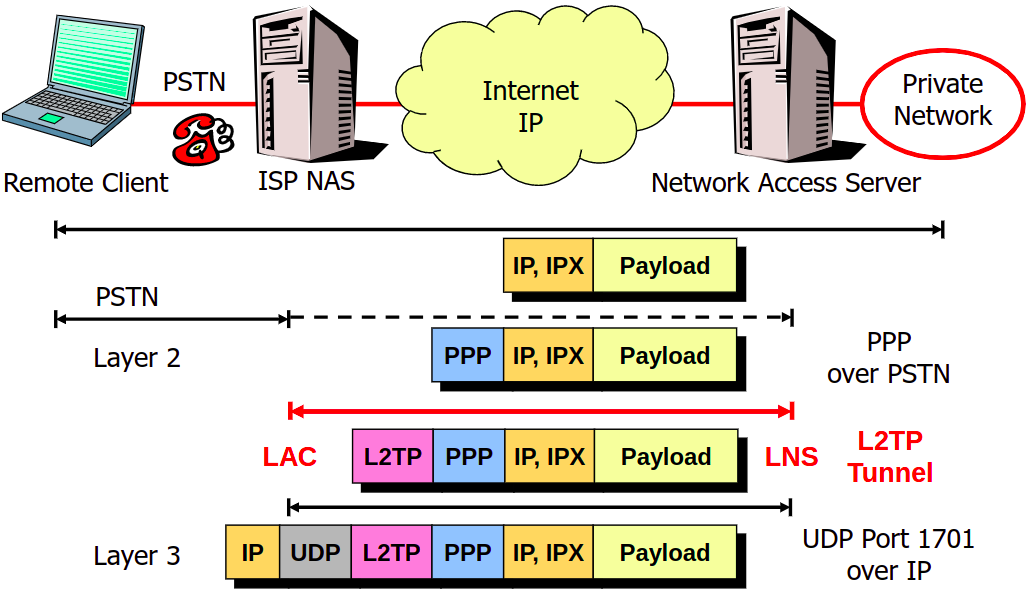
\includegraphics[width=\linewidth]{images/l2tp-compulsary-mode.png}
    	    	\caption{Compulsary Mode}
            	\end{minipage}
        	\begin{minipage}[t]{0.4\textwidth}
            		\centering
            		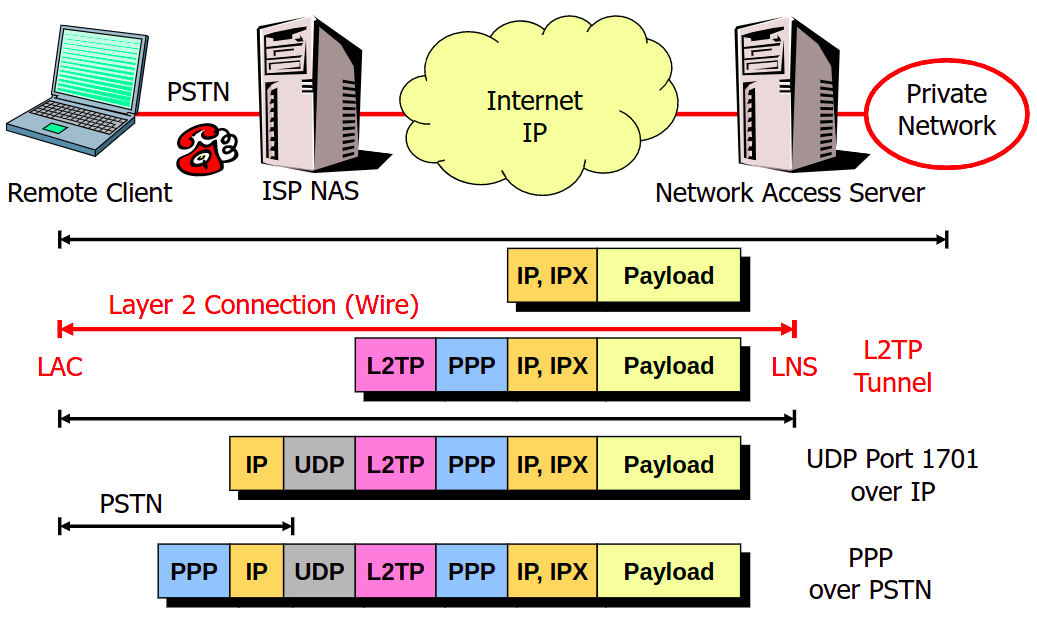
\includegraphics[width=\linewidth]{images/l2tp-voluntary-mode.png}
            		\caption{Voluntary Mode}
        	\end{minipage}
        \end{figure}
	    \item  Layer 3 Tunnel mit IPsec - Aufbau eines sicheren Tunnels auf Layer 3, es können jedoch nur IP Protokolle getunnelt werden
	    \newpage
	    \item L2TP over IPsec - Der IPsec Transport Mode wird verwendet, um die enkapsulierten Layer 2 Frames zu sichern/verschlüsseln.
	    
    	    \begin{minipage}[t]{0.4\textwidth}
    		\centering
    		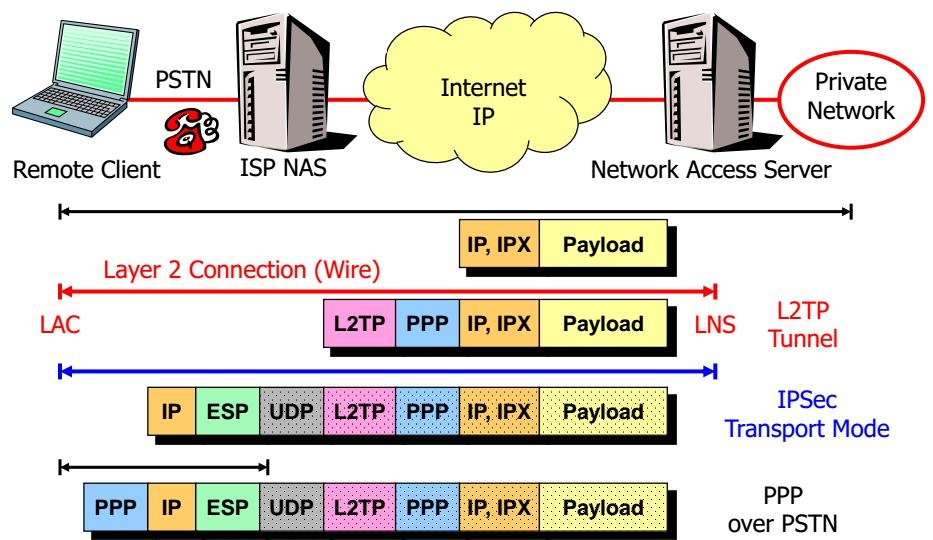
\includegraphics[width=\linewidth]{images/l2tp_ipsec_remote_access}
    	    \end{minipage}
	    \item Layer 4 Tunnel mit TLS (Transport Layer Security).
	\end{itemize}
	\item[SSL VPN] Erlaubt verschlüsselten Fernzugriff auf Unternehmensanwendungen um auf entfernte Ressourcen gesichert zuzugreifen.
	
		\begin{minipage}[t]{0.4\textwidth}
		\centering
		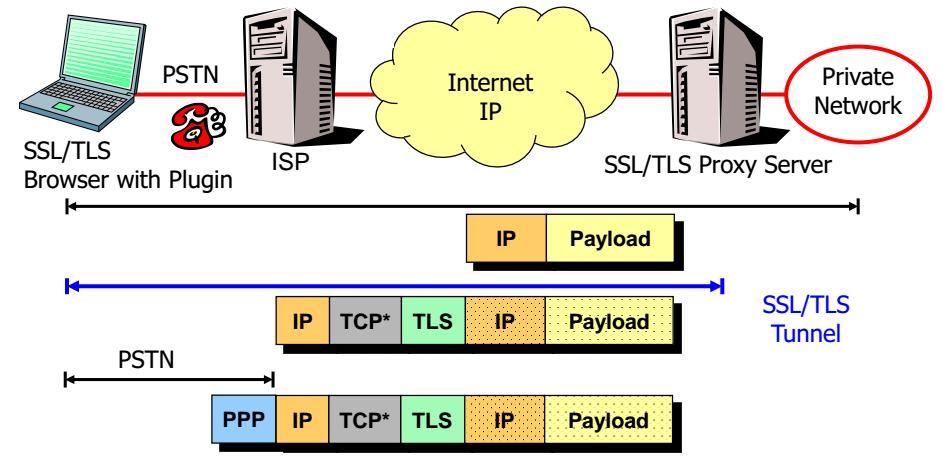
\includegraphics[width=\linewidth]{images/l4_tls_tunnel}
	\end{minipage}
\end{description}

\subsubsection{Vor- und Nachteile}
\begin{itemize}
    \item Layer 2 - L2TP
    \begin{itemize}
        \item[+] Gleiche Login Prozedur wie bei PPP (preshared key, RADIUS, etc.)
        \item[+] Gleiche Zusatzinformationen wie bei PPP( virtuelle IP, DNS/WINS server)
        \item[-] Keine Sicherheit ohne IPSEC, Session Hijacking oder Replay Attacken möglich
\end{itemize}
\item Layer 3 - IPsec
\begin{itemize}
    \item[+] Starke Verschlüsselung und Authentifizierung des Tunnels
    \item[+] Möglichkeit komplexe Zugriffsrichtlinien zu implementieren (z.B mit strongSwan)
    \item[+] XAUTH- und IKEv2-EAP-Authentifizierung bringen PPP-ähnliche Funktionen
    \item[-] Keine Unterstützung von nicht IP-Protokollen
    \item[-] Komplexes Setup/Verbindungsaufbau
\end{itemize}
\item Layer 4 - TLS
\begin{itemize}
    \item[+] Keinen Client benötigt, einfach (z.B nur Browser benötigt)
    \item[+] Starke Verschlüsselung und Authentifizierung des Tunnels
    \item[-] Gewisse Applikationen brauchen Plugins (nicht kompless clientsless)
\end{itemize}
\end{itemize}

\subsection{MPLS-VPN: Multi-Protocol Label Switching}
MPLS ist ein Verfahren, welches vor allem Internet Service Provider in ihrem Backbone anwenden. Dabei erhalten Kunden ein eindeutiges Label zugeordnet. Mit diesem Laber erreicht der ISP eine logische Trennung der Kunden. Jedoch ist standardmässig nichts verschlüsselt. MPLS Kunden müssen daher eine VPN Lösung (z.B. IPsec) verwenden oder einen Verschlüsselungs-Service vom Provider kaufen. Beide Varianten sind sehr weit verbreitet. 

\subsection{IPsec: Internet Protocol Security}\label{sec:ipsec-internet-protocol-security}
\begin{figure}[h]
\centering
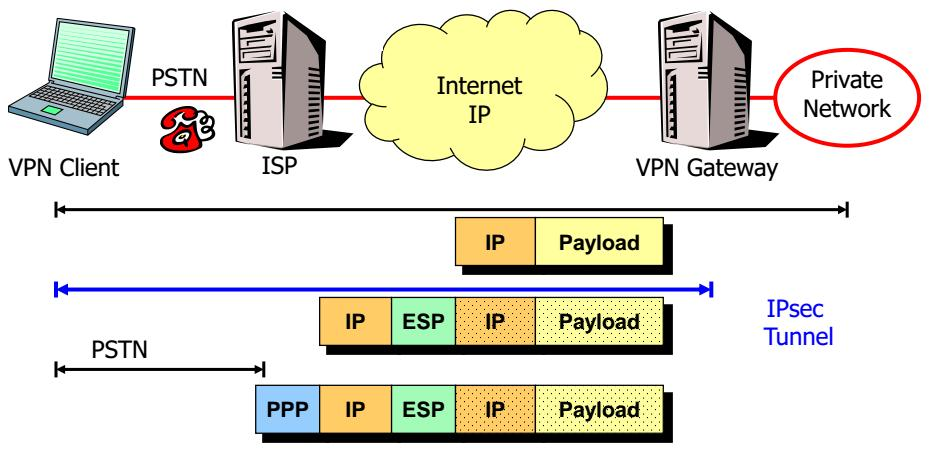
\includegraphics[width=0.7\linewidth]{images/ipsec_remote_access}
\caption{IPsec Remote Access}
\label{fig:ipsecremoteaccess}
\end{figure}

\begin{itemize}
	\item IPsec ist eine Protokoll Suite (Bausatz). Dass heisst, man kann die einzelnen Teile miteinander kombinieren.
	\item IPsec definiert die Vorgehensweise für die Datenintegrität, die Vertraulichkeit der Inhalte sowie die Verwaltung der kryptografischen Schlüssel. Es besteht aus folgenden Bausteinen
	\begin{description}
		\item[AH] Authentication Header
		\item[ESP] Encapsulating Security Payload
		\item[SA] Security Association
		\item[SPI] Security Parameter Index (32Bit): Identifier der SA
		\item[IKE] Internet Key Exchange (Siehe Sektion \ref{sec:ike})
	\end{description}
	\item Bei IPsec wird unterschieden zwischen
	\begin{itemize}
	    \item Transport Mode - Es wird ein IPsec Tunnel zwischen zwei Endgeräten (z.B PCs) aufgebaut
	    \item Tunnel Mode - Es wird ein IPsec Tunnel zwischen zwei Security Gateways (z.B Next Generation Firewalls) aufgebaut.
	\end{itemize}
	Dabei gibt es verschiedene Arten wie ein IPsec VPN aufgebaut werden kann. Entweder mit der Authentication-Header (AH) Methode oder mit der ESP Methode.
	
        	\begin{minipage}[t]{0.4\textwidth}
        		\centering
        		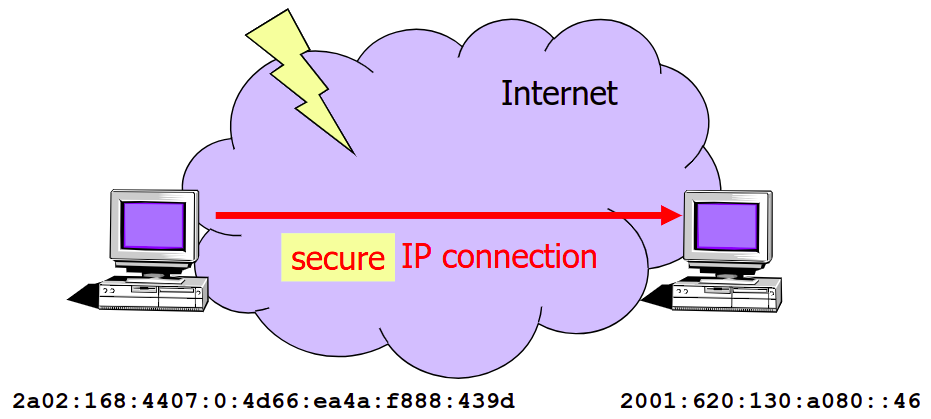
\includegraphics[width=\linewidth]{images/ipsec_transport-mode.png}
    	    	\caption{Transport Mode}
            	\end{minipage}
        	\begin{minipage}[t]{0.4\textwidth}
            		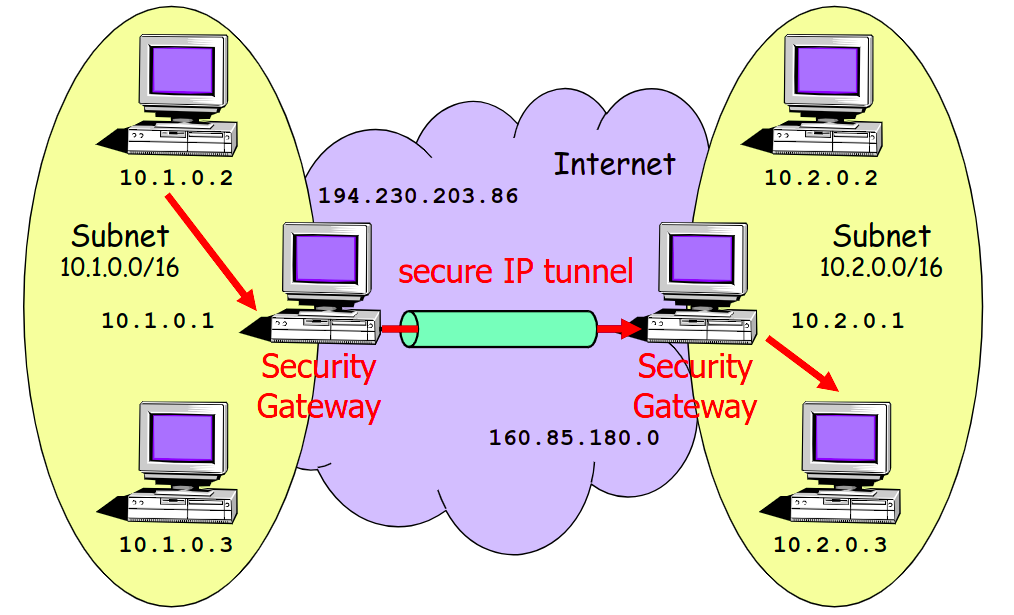
\includegraphics[width=\linewidth]{images/ipsec_tunnel-mode.png}
            		\caption{Tunnel Mode}
        	\end{minipage}
	
	\item Path MTU Discovery muss funktionieren. Somit kann IPsec den korrekten Overhead von der MTU abziehen und sendet so nie eine zu grosse MTU, die dann auf dem Weg gedropt wird. (Bsp. Ping funktioniert, Grösserer Download nicht $\rightarrow$ MTU Einstellungen prüfen, oder MTU manuell setzen.)
	\item IPsec hat seine Stärke besonders bei der Performance.
	\item Der äussere IP Header dient dem Routing zwischen den beiden VPN Gateways, Der innere IP Header beinhaltet die IP Adressen der beiden Clients.
\end{itemize}

\subsubsection{AH: Authentication Header}
\begin{itemize}
	\item Meist als zusätzlicher IP-Header verpackt: IP Protokoll Nr. 51
	\item Es ist für die Authentizität und Integrität der übertragenen Pakete zuständig authentifiziert den Server
	\item Es schützt gegen Replay Attacken
	\item Der AH schützt das komplette Paket vor Veränderungen ist jedocht \textbf{nicht verschlüsselt}. (Ausgenommen sind Felder die auf dem Weg verändert werden. z.B TTL, ToS, Fragment Offset, IP Header Checksum)
	\item Ein Nachteil von AH ist, dass es inkompatibel mit NAT ist, da NAT Teile des IP Headers ändert, die gemäss AH nicht verändert werden dürfen.
	\item Nicht so oft verwendet, da es die Daten nicht verschlüsselt. Eine Alternative wäre die Verwendung von ESP in AH, ist jedoch nicht weit verbreitet.
\end{itemize}

\begin{figure}[ht!]
    \centering
	\begin{minipage}[t]{0.45\textwidth}
        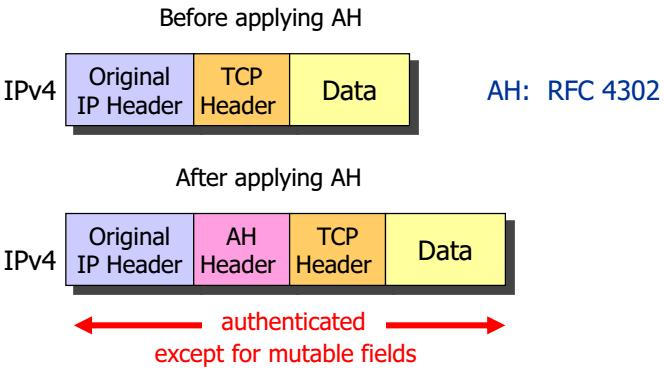
\includegraphics[width=\linewidth]{images/ipsec_ah_header}
        \caption{AH Transport Mode}
    \end{minipage}
	\begin{minipage}[t]{0.5\textwidth}
        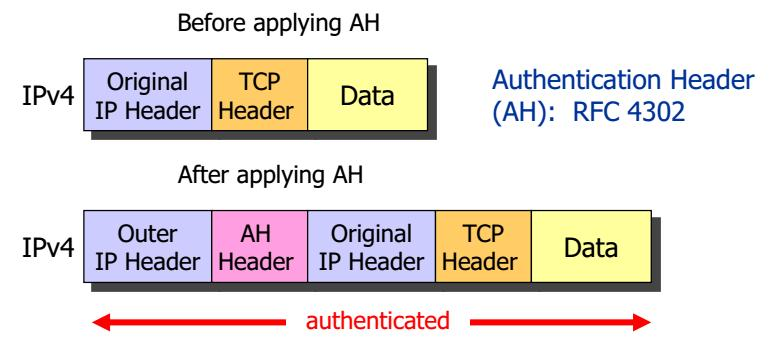
\includegraphics[width=\linewidth]{images/ipsec_ah_transport}
        \caption{AH Tunnel Mode}
    \end{minipage}
\end{figure}





\subsubsection{ESP: Encapsulating Security Payload}
\begin{itemize}
	\item Ein zusätzlicher Header und Trailer um den Layer 4 Payload.
	\item IP Protokoll Nr 50 (Kein Port $\rightarrow$ Kein NAT, ausser ESP in UDP gepackt)
	\item Ist für die Sicherstellung der Authentizität, Integrität und Vertraulichkeit von IP Paketen zuständig
	\item Die Nutzdaten, Padding, Pad Lenght und Next Header werden \textbf{verschlüsselt}
	\item Wird ESP Auth. verwendet, ist der IP Header nicht geschützt, jedoch ist das kein Nachteil: IP Spoofing ist nicht möglich. Oft verwendet anstatt AH.
	\item Im Unterschied zum AH wird der Kopf des IP-Paketes vom \textit{icv} (integrity check value)) nicht authentifiziert.
\end{itemize}

\begin{figure}[ht!]
    \centering
	\begin{minipage}[t]{0.45\textwidth}
        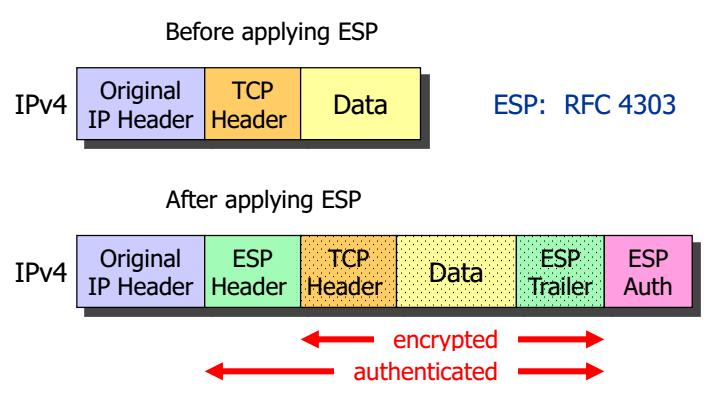
\includegraphics[width=\linewidth]{images/ipsec_esp}
        \caption{ESP Transport Mode}
    \end{minipage}
	\begin{minipage}[t]{0.5\textwidth}
        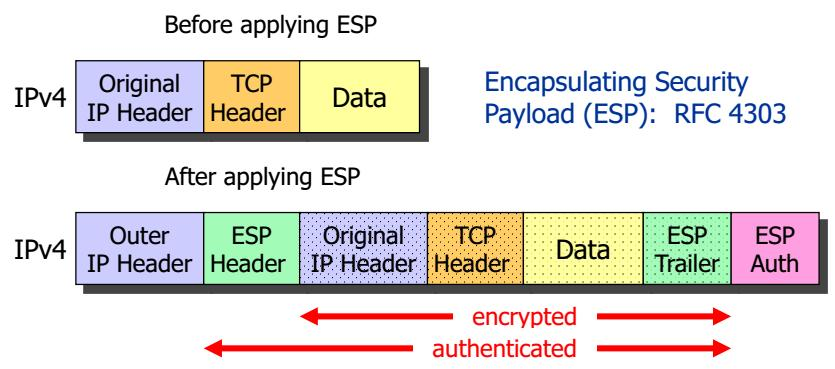
\includegraphics[width=\linewidth]{images/ipsec_esp_tunnel}
        \caption{ESP Tunnel Mode}
    \end{minipage}
\end{figure}


\paragraph{NAT} \hfill \\
Mit der NAT Traversal Extension werden ESP Pakete in UDP verpackt, welche dann problemlos von NAT gemappt werden könnnen. Zusätzlich werden die Daten neu an Port 4500 gesendet, damit alte NAT-Router kein IP-Basiertes Traversal machen. Der Grund dafür ist, dass ESP ein eigenständiges L3 IP Protokoll (50) ist und somit keine Ports besitzt.
\begin{figure}[h]
\centering
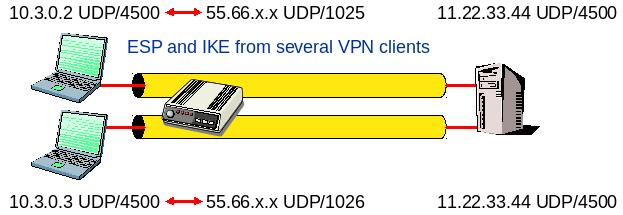
\includegraphics[width=0.5\linewidth]{images/ipsec_nat}
\caption{IPsec NAT}
\label{fig:ipsecnat}
\end{figure}

\subsection{StrongSwan}
Bei der Konfiguration von StrongSwan muss beachtet werden dass \textbf{local} die \textbf{lokale Domäne} und \textbf{remote} für den \textbf{Remote} steht. Beim GW ist also local der GW selber und remote der Client, beim Client ist local er selber und remote der GW.
\begin{description}
	\item[/etc/ipsec.d/cacerts] CA Zertifikate
	\item[/etc/ipsec.d/certs] User Zertifikate
	\item[/etc/ipsec.d/private] User Keys
	\item[/etc/ipsec.secrets] : ECDSA userKey.pem "your\_secrete\_pw"
\end{description}

\begin{lstlisting}[caption=/etc/ipsec.conf]
conn %default  
	leftcert=loginCert.pem // Cert das an die Gegenstelle gesendet wird
	// leftid = Per default distinguished name aus Cert

conn gateway-net 
	also=gateway // reuse content of "gateway" connection
	rightsubnet= 10.5.0.0/16

conn gateway 
	right= 152.96.31.50 // ip adresse der Gegenstelle
	rightid=intsec.hsr.ch 
	auto=add
	
ca hsr 
	cacert=hsrCert.pem
	ocspuri=http://intsec.hsr.ch:8880
	auto=add
\end{lstlisting}

\begin{figure}[h]
\centering
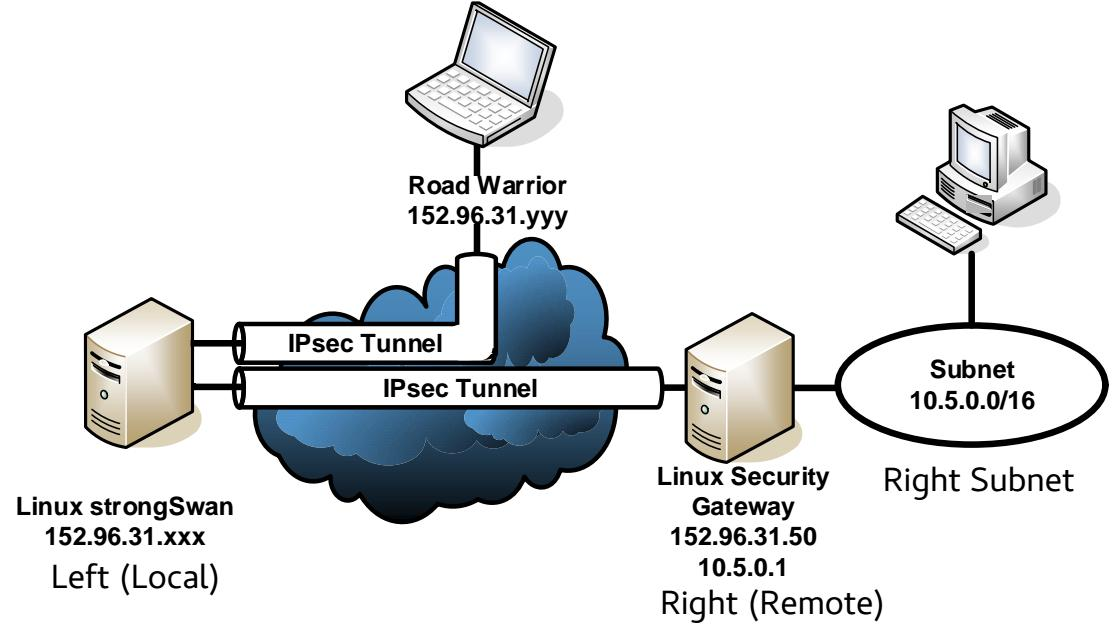
\includegraphics[width=0.4\linewidth]{images/ipsec_aufbau}
\caption{strongSwan Üubungs Aufbau}
\label{fig:ipsecaufbau}
\end{figure}

\subsubsection{Konfiguration swanctl.conf}
\begin{description}
    \item[Connections Sektion (enthält Subsektionen für jede IKE Verbindung)] ''remote\_addrs'' gibt die IP-Adresse oder den Hostnamen der Gegenstelle an. Als Responder können optional mehrere angegeben werden (auch in CIDR- oder Range-Notation), von denen dann Verbindungen akzeptiert werden (wird die Option auf Respondern weggelassen, kann die IP-Adresse der Clients beliebig sein).
    \item[local/remote Sektion (für Authentisierungsoptionen konfigurieren)] ''local.certs'' gibt den Pfad auf das eigene Zertifikat an, das an die Gegenstelle gesendet werden soll (dies ist eine kommagetrennte Liste von Pfaden, entweder relativ zum x509 Verzeichnis oder absolut). 
    \begin{itemize}
        \item \textbf{''local.id''} konfiguriert die eigene Identität, die an die Gegenstelle gesendet wird. Fehlt die Option, so wird per Default der Distinguished Name aus dem ersten Zertifikat extrahiert (bzw. auf die IP-Adresse zurückgegriffen, falls keines konfiguriert wurde).
        \item \textbf{''remote.id''} konfiguriert die Identität der Gegenstelle. Wir wählen hier eine ID\_FQDN d.h. einen Hostnamen. Das Zertifikat der Gegenstelle muss damit den Hostnamen als subjectAlternativeName Extension enthalten.  Fehlt die Option, gilt dasselbe wie für die eigene Identität.
    \end{itemize}
    \item[Child-SAs] ''remote\_ts'' definiert das Subnetz das hinter dem VPN Gateway der Gegenseite liegt, in der Form x.y.z.u/Bitmaske (TS steht für Traffic Selector, da optional auch nach Port und Protokoll selektiert werden kann). Mit IKEv2 können mehrere, durch Komma getrennte, TS konfiguriert werden. Ist die Option nicht definiert, wird die Remote IP verwendet. Gleiches gilt für ''local\_ts'', also die eigenen Traffic Selectors, die wir hier für beide CHILD\_SAs bei der eigenen IP belassen. Die Host-SA existiert immer und beinhaltet immer implizit die virtuelle IP oder die die remote\_addrs.
    \item[Virtuelle IP] Der Client bekommt eine virtuelle IP aus dem Subnet 10.4.0.0/24 (10.4.0.36). Er braucht eine virtuelle IP, damit wenn der Gateway den Traffic ins Zielnetz weiterleitet, muss das Zielnetz auch wissen wohin es antworten soll. Wenn der Client nun einfach eine private IP hätte, könnte diese von mehreren verbundenen Clients verwendet werden, was natürlich zu einem Routing Problem führen würde (z.b. 2 mal IP 192.168.1.50). Falls der Client eine öffentliche IP hätte, würde der Traffic über das öffentliche Netz und nicht über den VPN Gateway zurückgeroutet werden! \lstinline|vids = 0.0.0.0| sagt dass der Client keine spezielle virtuelle IP vom GW will, dann nimmt er die die er vom GW bekommt.
\end{description}


\subsubsection{Beispiel}
Für einen fixen Tunnel zwischen zwei Netzwerken (auf den Routern \lstinline|deviceA| und \lstinline|deviceB|)

\paragraph{deviceA} \hfill \\
\begin{lstlisting}
conn %default
	ikelifetime=60m
	keylife=20m
	rekeymargin=3m
	keyingtries=1
	authby=secret
	keyexchange=ikev2
	mobike=no

conn net-net
	left=deviceA.hsr.ch
	leftsubnet=192.168.1.0/24
	leftid=@deviceA.hsr.ch
	leftfirewall=yes
	lefthostaccess=yes
	right=deviceB.hsr.ch
	rightsubnet=192.168.2.0/24
	rightid=@deviceB.hsr.ch
	auto=route
\end{lstlisting}

\paragraph{deviceB} \hfill \\
\begin{lstlisting}
conn %default
	ikelifetime=60m
	keylife=20m
	rekeymargin=3m
	keyingtries=1
	authby=secret
	keyexchange=ikev2
	mobike=no

conn net-net
	left=deviceB.hsr.ch
	leftsubnet=192.168.2.0/24
	leftid=@deviceB.hsr.ch
	leftfirewall=yes
	lefthostaccess=yes
	right=deviceA.hsr.ch
	rightsubnet=192.168.1.0/24
	rightid=@deviceA.hsr.ch
	auto=route
\end{lstlisting}

\subsection{Prüfungsaufgabe}
\paragraph{Topologie} \hfill
\newline
	\begin{minipage}[t]{0.8\textwidth}
        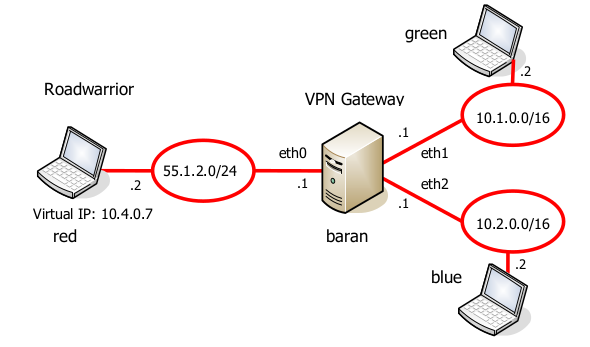
\includegraphics[width=\linewidth]{images/hs18-19-ipsec-topology.png}
    \end{minipage}

Der Roadwarrior red baut mittels IKEv2 zwei CHILD SAs zum Gateway baran auf. In beiden
VPN Endpunkten wird strongSwan eingesetzt. Die Konfiguration sieht wie folgt aus:

\paragraph{swanctl.conf auf red}
\begin{lstlisting}
connections {
    to-baran {
        version = 2
        local_addrs = 55.1.2.2
        remote_addrs = 55.1.2.1
        vids = 0.0.0.0
        local {
            certs = redCert.pem
            id = red@colors.net
        }
        remote {
            id = baran.colors.net
        }
        children {
            host {
            }
            net {
                remote_ts = 10.0.0.0/14
            }
        }
    }
}
\end{lstlisting}

\paragraph{swanctl.conf auf baran}
\begin{lstlisting}
swanctl.conf auf baran :
connections {
    from-red {
        version = 2
        local_addrs = 55.1.2.1
        pools = red-vip
        local {
            certs = baranCert.pem
            id = baran.colors.net
        }
        remote {
            id = red@colors.net
        }
        children {
            host {
            }
            net {
                local_ts = 10.1.0.0/16
            }
        }
    }
}
pools {
    red-vip {
        addrs = 10.4.0.7
    }
}
\end{lstlisting}


\begin{minipage}[t]{0.8\textwidth}
        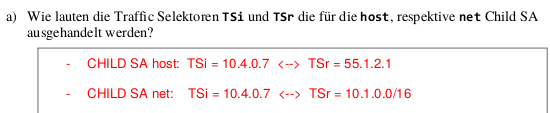
\includegraphics[width=\linewidth]{images/hs18-19-ipsec-exc1.png}
\end{minipage}

\begin{minipage}[t]{0.8\textwidth}
        \includegraphics[width=\linewidth]{images/hs18-19-ipsec-exc2.png}
\end{minipage}


\begin{minipage}[t]{0.8\textwidth}
        \includegraphics[width=\linewidth]{images/hs18-19-ipsec-exc3.png}
\end{minipage}


\section{IKE: Internet Key Exchange}\label{sec:ike}
\subsection{Grundlagen}
Für den IPsec Verbindungsaufbau ist das sogenannte Internet Key Exchange Protokoll zuständig. Seit 2005 kann das verbesserte IKEv2 verwendet werden. 4 Jahre später war Windows 7 die erste kommerziell verfügbare Implementierung des Standards.
\begin{itemize}
	\item Das \textit{ike} Protokoll ist für den Aufbau einer \textit{sa} (Security Association) zuständig. Eine SA muss \textbf{einmal für jede Richtung (unidirektional)} ausgehandelt werden.
	\item Das Protokoll dient der Verwaltung und zum Austausch der Schlüssel in IPsec. Zusätzlich bietet es ein standardisiertes Verfahren für die Authentifizierung von Kommunikationsparter sowie zur Erzeugung von gemeinsam genutzten Schlüsseln.
	\item UDP Port 500 (Socketverbindung) / 4500 (Übertragung)
	\item Aktuell gibt es zwei Versionen von IKE: Version 1 arbeitet in zwei Phasen und Version 2 braucht viel weniger Meldungen für den Verbindungsaufbau. 
\end{itemize}

\subsubsection{Security Association}
\begin{description}
    \item [Security Association] Eine Security Association, kurz SA, ist ein Contract/Vertrag der zwischen zwei IPsec Endpunkten abgeschlossen wird. Die Endpunkte können dabei ein Security Gateway oder ein Host sein.
    \item [Aushandelte Parameter] Innerhalb dieser SA werden verschiedene Parameter ausgehandelt, welche für den IPsec Verbindungsaufbau gebraucht werden:
    \begin{itemize}
        \item Authentifizierungsmechanismus (bei IKEv1 nur PSK oder public key)
        \item Verschlüsselungalgorithmun, Datenintegritätsalgorithmus, PRF
        \item Schlüsselaustausch mittels DH-Gruppen
        \item Schlüssel Lebensdauer (nur bei IKEv1) für ISAKMP und IPsec SAs
    \end{itemize}
    \item [Schutz des Aushandlung] ISAKMP SA (IKEv1) oder IKE SA (IKEv2) schützt die IKE-Verhandlung.
    \item [Seperate SAs] Separate IPsec SA (IKEv1) oder CHILD SA (IKEv2) sind für jedes Subnetz oder jeden einzelnen Host erforderlich (IKEv2 erlaubt die Verkettung von SAs).
\item [Eindeutige SPIs] Jede IPsec SA erhält \textbf{für jede Richtung (inbound/outbound)} einen einedeutigen SPI (Security Parameter Index).
    \end{description}
\subsection{Version 1}
\begin{itemize}
	\item ISAKMP\_SA handelt die Paramter für die IKE Übertragung selbst aus.
	\item Verwendet Pre-Shared Secrets oder Public Key
	\item Verwendet XAUTH zur erweiterten Authentisierung (Überträgt Passwort im Klartext)
	\item Ein Verbindungsaufbau zwischen zwei Endstations benötigt 15 Meldungen.
	\[
	12 = 6 (Phase 1) + 3 (Phase 2: Richtung A) + 3 (Phase 2: Richtung B)
	\]
\end{itemize}

\subsubsection{Ablauf}
In der Version 1 wird der IPsec Verbindungsaufbau in zwei Phasen eingeteilt:
\begin{enumerate}
	\item In einer ersten Phase baut IKE eine Verbindung mit relativ schwachen Sicherheitsmechanismen auf, die der Absicherung und Authentifizierung der weiteren Verwaltungsvorgänge dient. Nach der ersten Phase steht eine ISAKMP\_SA, welche bidirektional ist. Dieser Schritt benötigt 6 Pakete (ausser im Agressive Mode)
	\item In einer zweiten Phase wird das zu verwendende Sicherheitsprotokoll ausgehandelt und umgesetzt. Dazu wird der in der Phase 1 erstellte Tunnel verwendet. Für diese Phase werden für \textbf{jede Richtung} je 3 Pakete verwendet. Es resultiert eine ESP SA über welche dann die wirklichen Daten übertragen werden.
	\begin{itemize}
		\item Zuerst schlägt der Client seine unterstützten Cipher Suites vor
		\item Das Gateway antwortet dann mit seiner Auswahl
		\item In dieser Phase werden auch die DH Schlüssel generiert
	\end{itemize}
\end{enumerate}


\subsubsection{Phase 1: Modes}
In einer ersten Phase handelt IKE die Parameter für die ISAKMP\_SA aus. Dabei gibt es verschiedene Modes:
\begin{description}
	\item[Main Mode] Das Problem beim Main Mode ist die Performance. Zusätzlich besteht das Problem, dass ein MitM Angreifer den Session Key des DH Exchange abfangen kann, da die ersten 4 Pakete im \textbf{Klartext} übertragen werden. Das Zertifikat wird in den letzten beiden Paketen übertragen.
	\item[Main Mode mit Pre Shared Keys] Die ersten vier Pakete sind gleich wie im Main Mode. Zusätzlich wird das Password (\textit{psk}) in den Hash eingearbeitet. Dies verhindert einen MitM Angriff. Ebenfalls ist somit die Indentität verschlüsselt.
	\item[Agressive Mode mit Pre Shared Keys] Beim Aggressive Mode ist das Ziel möglichst schnell die Phase 1 abzuarbeiten. Man schickt deshalb mehr Informationen pro Paket. Das grosse Problem ist, dass die Nachrichten unverschlüsselt übertragen werden. PSK mit anderen Parameter wird in den Hash gegeben, somit sind offline-cracking Attacken möglich.
\end{description}

\begin{figure}[ht!]
\begin{minipage}[t]{0.5\textwidth}
		\centering
		\includegraphics[width=\linewidth]{images/ike_v1_main_mode}
		\caption{IKE Main Mode}
	\end{minipage}
	\begin{minipage}[t]{0.5\textwidth}
		\centering
		\includegraphics[width=\linewidth]{images/ike_v1_main_mode_presharedkeys}
		\caption{Main Mode mit Pre-Shared Keys}
	\end{minipage}

\end{figure}
	\newline
\begin{figure}
	\begin{minipage}[t]{0.9\textwidth}
		\centering
		\includegraphics[width=0.7\linewidth]{images/ike_v1_aggressive_mode_presharedkeys}
		\newline
		\caption{Agressive Mode mit Pre-Shared Keys}
	\end{minipage}
\end{figure}


\subsubsection{Phase2: Quick Mode}
In der Phase zwei wird folgendes gemacht:
\begin{itemize}
    \item Mit 3 weiteren Paketen wird eine IPsec SA erstellt. Dazu wird der sichere Kanal verwendet, welcher in Phase 1 (ISAKMP\_SA) erstellt wurde über den sicheren Kanal, welcher in Phase1 erstellt wurde.
    \item Die spezifischen Konfigurationsparameter für die IPsec-Verbindung werden ausgehandelt (AH, ESP, Authentifizierungs-Verschlüsselungsverfahren und -parameter).
    \item Diese Phase kann ebenfalls verwendet werden, um auslaufende IPsec SAs zu erneuern.
    \item Die ESP-Verschlüsselung und die ESP/AH-Authentifizierungsschlüssel für die IPsec-SAs werden aus dem Phase 1 Diffie-Hellman-Secret abgeleitet.
    \item Optional können bei jedem Quick Mode neue DH-Parameter generiert werden (perfect forward secrecy). 
\end{itemize}

\subsection{Version 2}
\begin{itemize}
	\item IKEv2 verwendet standardmässig nur 1024Bit DH für den Schlüsselaustausch. 
	\item IKE SA ist das v2 Pendant zum ISAKMP\_SA unter v1
	\item IKE v2 ist komplett neu, bis auf den Port 500 - keine Rückwärtskompatibiliät
	\item IKE v2 verfügt über die Möglichkeit Child SA zu erstellen. Dies wird besonders beim Re-Keying verwendet.
	\item Verwendet \textit{eap} zur erweiterten Authentisierung
	\item IKE v2 unterstütz Cookie Mechanismus gegen DoS Attacken (nicht aber gegen DDoS, da die Zombies die Cookies zurücksenden)
	\item Bei IKEv2 wurde auf einen präventiven Cookie-Austausch verzichtet (Es gibt selten Probleme mit DOS). Der Cookie Mechanismus kann jedoch manuell aktiviert werden. 
	\item Nur noch 4 anstatt den 9 Meldungen in V1
	\item Ein Verbindungsaufbau zwischen zwei Endstations benötigt 6 Meldungen:
	\[
	6 = \text{4 (je 2 für IKE\_SA und IKE\_AUTH: beinhaltet bereits eine Child SA!) + 2 (Child SA)}
	\]
\end{itemize}


\begin{figure}[ht!]
	\centering
	\begin{minipage}[t]{0.4\textwidth}
		\centering
		\includegraphics[width=\linewidth]{images/ike_v2}
		\caption{IKE V2: First Child SA}
		\label{fig:ikev2}
	\end{minipage}
	\begin{minipage}[t]{0.4\textwidth}
		\centering
		\includegraphics[width=\linewidth]{images/ike_v2_additional_sa}
		\caption{IKE V2: Additional Child SA}
		\label{fig:ikev2additionalsa}
	\end{minipage}
\end{figure}

\subsubsection{Ablauf}
\begin{itemize}
	\item IKE\_SA\_INIT Request und Response im Klartext
	\begin{itemize}
		\item Im SA Payload sind die ausgehandelten Cipher Suites sichtbar
		\item Crypto Parameter( vorgeschlagene Krypto-Suites, öffentlicher DH-Faktor, Initiator Nounce) werden in den Request aufgenommen, der Responder wählt die für ihn besten aus.
	\end{itemize}
	\item IKE\_AUTH Request und Response (Erstellt SA zum Gateway)
	\item CREATE\_CHILD\_SA Request und Response (Erstellt SA vom Gateway ins Netz hinter dem Gateway)
\end{itemize}

\subsubsection{Cookie Mechanismus gegen DoS Attacken}
IKEv2 bietet einen sogenannten Cookie Mechanismus gegen DoS Attacken an. Der Security Gateway kann sich die halb-offenen IKE\_SAs merken und so bei zu vielen IKE Pakete merken, dass er unter DoS Attacke ist und so die IKE Pakete verwerfen. Ebenfalls ist es möglich halb offene IKE\_SAs nach einem definierten Timeout zu schliessen.

\subsubsection{Narrowing}
Narrowing vereinfacht die Konfiguration von IKEv2 um ein Vielfaches. Beim Narrowing wird automatisch das kleinste Subnetz genommen.

\section{DNSSEC: DNS Security Extensions}

\subsection{DNS}
\begin{itemize}
	\item DNS basiert auf UDP und ist deshalb ohne erweiterten Sicherheitsmassnahmen (Source Port Randomization und Query ID Randomzation) einfach zu spoofen.
	\item Rekursive Auflösung: Bei der rekursiven DNS Server fragt der lokale Namensserver rekursiv alle benötigten externen Nameserver an, um die Adresse aufzulösen.
	\item Der Source Port ist im Standard nicht definiert. Der Destination Port von DNS ist immer 53
	\item Die QID (16 Bit Query ID) identifiziert einen DNS Request. Sie muss gleich wie die DNS Response Transaction ID sein.
	\item Query ID und Source Port müssen passen, damit ein DNS Server einen Request beantwortet.
\end{itemize}
\begin{figure}[ht!]
	\centering
	\begin{minipage}[t]{0.5\textwidth}
		\centering
		\includegraphics[width=\linewidth]{images/dns_request}
		\caption{DNS Request}
		\label{fig:dnsrequest}
	\end{minipage}
	\begin{minipage}[t]{0.5\textwidth}
		\centering
		\includegraphics[width=\linewidth]{images/dns_response}
		\caption{DNS Response}
		\label{fig:dnsresponse}
	\end{minipage}
\end{figure}

\subsection{DNS Cache Poisoning}
Beim DNS Cache Poisoning versucht ein Angreifer die Query ID und den Source Port zu erraten und dabei eine schnellere Antwort zu liefern, als der korrekte Nameserver. Der erste DNS Response der beim Client NS ankommt, wird in den Cache geschrieben und alle weitere Anfragen laufen dann, im schlimmsten Fall über den NS des Angreifers. Hat er sein Ziel erreicht, kann er alle DNS Requests und MX Records für eine Zone manipulieren.

\subsection{DNSSEC Resource Records}
Mit DNSsec kann man sicher gehen, dass die zurückgelieferten DNS Records vertrauenswürdig sind. Dazu muss man einzig dem KSK der Root Zone vertrauen. Dieser muss im DNS Resolver hinterlegt werden.
\begin{description}
	\item[KSK: Key Signing Key (Flag=257)] langfristiger Schlüssel (2048Bit RSA). Mit dem KSK wird wird der ZSK signiert.
	\item[ZSK: Zone Signing Key (Flag=256)] Mit diesem werden alle Zone Records signiert. Dies wird bei jeder Generierung des Zonen-Files gemacht. (1024Bit RSA). Mit dem ZSK werden die DS Records der darunterliegenden Zonen signiert. (Root $\rightarrow$ Top Level $\rightarrow$ .. ) 
	\item[DS: Delegation Signer] 
	Der DS Record ist ein Hash über den Public Key (KSK) der darunter liegenden Zone. Erstellt man mit dem definierten Hash Algorithmus einen Hash über den Public Key kann dieser mit dem DS Record verglichen werden.
	\begin{lstlisting}[caption=DNSKEY]
	domain.ch. <time to live> IN DNSKEY <flag> 3 <algorithm>
	<base 64 public_key>; {id=<key tag id> (zks|ksk), size = <size>}
	\end{lstlisting}
	\item[RRset] Mittels RRsets werden alle Records des gleichen Typs gruppiert. Beispielsweise bilden alle A-Records sowie alle MX-Records je ein Set.
	\item[DNSKEY] Ist ein Base64 codierter Public Key. Mit diesem wird die RRSIG Signatur wieder entschlüsselt. Daraus resultiert ein Hash. Mit dem gegebenen Hash Algorithmus muss der RRset (z.B A Record) gehashed werden. Sind die beiden Hashes gleich, kann dem DNS Server vertraut werden.
	\item[RRSIG: Resource Record Signature] Enthält die Signatur über ein RRset (z.B A Record, IPSECKEY Record oder DS Record)
	\begin{lstlisting}[caption=RRSIG]
	sub.domain.ch. <time to live> IN RRSIG <record_type> <algorithm> 3 <time to live>
	<valid from>
	<valid to>
	<key tag id> <parent domain>
	<signature>
	\end{lstlisting}
	\item[NSEC: Next Owner Name] Mit NSEC Records ist es möglich, alle Namen einer Zone aufzulisten. Man beginnt mit einer Anfrage nach einem NSEC Record bei einem bliebigen Namen und erhält damit den nächsten gültigen Namen. Seit Version 3 werden die Records mit gehashed. Man erhält also einen Hash zurück. Dieser kann nur noch mit einer Dictionary Attack geknackt werden.
\end{description}


\subsubsection{Ablauf: Chain of Trust}
\begin{enumerate}
	\item Die Zone \lstinline|switch.ch.| hat einen KSK (DNSKEY Eintrag) und einen ZSK (DNSKEY Eintrag). Der KSK signiert den ZSK. Der ZSK signiert alle weiteren DNS Records. Daraus resultieren RRSIG Einträge (Hashes)
	\item Die Zone \lstinline|.ch.|, hat ebenfalls einen KSK (DNSKEY Eintrag) und einen ZSK (DNSKEY Eintrag). Auch hier signiert der KSK den ZSK. Der ZSK signiert alle weiteren DNS Records. Auch hier resultieren RRSIG Einträge (Hashes)
	\item Damit dem KSK in der Zone \lstinline|switch.ch.| vertraut wird, muss diese manuell einen DS Eintrag in der darüberliegenden Zone (.ch.) erstellen. (Aufgabe des Sysadmin: Anfrage bei Top Level Zone)
	\item Dieser DS Eintrag wird vom ZSK der Zone ''.ch.'' signiert. Es resultiert wieder ein RRSIG Eintrag.
	\item Dies wird wiederholt bis am in der Root Zone angelangt ist.
\end{enumerate}

\begin{figure}[h!]
	\centering
	\includegraphics[width=0.9\linewidth]{images/dnssec_chainoftrust}
	\caption{DNSsec Chain of Trust}
	\label{fig:dnssecchainoftrust}
\end{figure}


\subsubsection{Verifikation}
Für die Verifikation muss der KSK der Root Zone, beim Client hinterlegt sein.
\begin{enumerate}
	\item Zuerst stellt der Client eine Anfrage für einen beliebigen Record an \lstinline|www.potaroo.net.|
	\item Die dafür zuständige Zone antwortet mit den geforderten Record und den RRSIG zu diesem Record. Um diesen RRSIG zu überprüfen wird der ZSK der Zone benötigt. 
	\item Der ZSK an sich muss aber auch überprüft werden. (Der könnte ja gefakt sein) Man überprüft deshalb den RRSIG des ZSK mit dem KSK der Zone
	\item Dem KSK kann aber auch nicht vertraut werden, solange er nicht verifiziert ist. Für den KSK existiert deshalb einen DS Eintrag in der darüberliegenden Zone. 
	\item Der DS Eintrag hat wiederum einen RRSIG Eintrag der mit dem ZSK der \lstinline|.net| Zone erstellt wurde.
	\item Die vorgehenden Schritte werden wiederholt, bis man bei der Root Zone ''.'' angekommen ist. Die Root Zone an sich wird mit dem beim Client hinterlegten KSK der Root Zone validiert.
\end{enumerate}


\begin{figure}[h]
	\centering
	\includegraphics[width=0.9\linewidth]{images/dnssec_verification}
	\caption{DNSSec Verifikation}
	\label{fig:dnssecverification}
\end{figure}

\clearpage

\subsection{Explicit Denial of Existence}
Wenn bei DNS nach d3er IP-Adresse einer Domäne gefragt wird die nicht existiert, wird eine leere Antwort zurückgegeben. Es gibt keine Möglichkeit, explizit zu antworten: "Die angeforderte Zone existiert nicht". Das ist ein Problem, wenn die Antwort authentifiziert sein soll, da keine Nachricht zu unterschreiben ist. DNSSEC behebt dies, indem es die Datensatztypen NSEC und NSEC3 hinzufügt. Beide erlauben eine authentifizierte Abstreitung der Existenz dieser Domäne. NSEC arbeitet mit der Rückgabe des "nächsten sicheren" Records. Wird beispielsweise ein Namenserver betrachtet, der AAAA-Datensätze für ein API, ein Blog und ein www deniert/bereitstellt. Betrachten wir beispielsweise ein Datensatz der für Store angefordert wird, so wird ein NSEC-Datensatz zurückgegeben, der www enthält. Das heiÿt, es gibt keine AAAA-Datensätze zwischen Store und www, wenn die Datensätze alphabetisch sortiert sind. Dies sagt eektiv aus, dass kein Store existiert. Und da der NSEC-Datensatz signiert ist, kann das entsprechende RRSIG wie jedes RRset validiert werden. Leider erlaubt diese Lösung jedem, durch die Zone zu gehen und jeden einzelnen Datensatz zu sammeln, ohne zu wissen, nach welchem er sucht. Dies kann eine potenzielle Sicherheitsbedrohung darstellen, wenn der Zonenadministrator den Inhalt der Zone als privat deklariert.

\subsection{DANE: DNS-based Authentication of Named Entities}
Mit DANE können Clients den DNS Server anfragen, welche TLS Zertifikate als vertrauenenswürdig eingestuft werden können. DANE erweitert somit TLS, dass die verwendeten Zertifikate \textbf{ nicht unbemerkt ausgewechselt} werden können. Dazu werden X.509 Zertifikate mit DNS Einträgen verknüpft und per DNSSec als TLSA Resource Record gesichert. Ausserdem können Domaininhaber eigene Zertifikate ausstellen und so die Dienste der CA's umgehen.

\subsubsection{Funktionsweise}
\begin{enumerate}
	\item Ruft ein Client eine Webseite auf, möchte er sich sicher sein, dass der korrekte Server die Webinhalte ausliefert. Dazu prüft er das Zertifikat des Servers
	\item Anschliessend muss er sicherstellen, dass das Zertifikat von einer vertrauenswürdigen CA ausgestellt wurde. Da es sehr viele CA's gibt, kamen Zweifel an der Verlässlichkeit der CA's auf. Hier setzt DANE an
	\item Clients können mit können mit DANE bei den DNS Server nachfragen, welche Zertifikate sie als vertrauenswürdig einstufen können. Dies wird über einen neuen TLSA Resource Record gemacht. Dieser enthält das Zertifikat und dessen Finger oder public Key. 
\end{enumerate}


\subsubsection{TLSA Resource Record}
\begin{figure}[h]
\centering
\includegraphics[width=0.7\linewidth]{images/tlsa_resource_record}
\caption{TLSA Resource Record}
\label{fig:tlsaresourcerecord}
\end{figure}

\begin{description}
	\item[Certificate Usage] \hfill
	\begin{itemize}
		\item 0 – CA Certificate Constraint
		\item 1 – Server Certificate Constraint
		\item 2 – Trust Anchor Assertion for Private CA
		\item 3 – Domain Issued Certificate
	\end{itemize}
	\item[Selector] \hfill
	\begin{itemize}
		\item 0 – Full Certificate
		\item 1 – Public Key Info (Public Key plus Key Type Information)
	\end{itemize}
	\item[Matching Type] \hfill
	\begin{itemize}
		\item 0 – Exact Match on Selected Content
		\item 1 – SHA-256 Hash of Selected Content
		\item 2 – SHA-512 Hash of Selected Content
	\end{itemize}
\end{description}

Mit der Distribution von Zertifikaten, öffentlichen Schlüsseln oder deren Hashes in RRs, kann DNSSEC auch für die Authentisierung von Hosts und darauf laufenden Anwendungen eingesetzt werden. Es gibt dabei vier Möglichkeiten Vertrauen in das Server-Zertifikat herzustellen: 
\begin{itemize}
    \item Man verweist auf ein CA Zertifikat, welches in der normal verifizierten Vertrauenskette vorkommen muss („CA constraint“ bzw. PKIX-TA)
    \item  Man referenziert das End-Entity-Zertifikat des Servers, dessen Vertrauenskette ansonsten normal verifiziert wird („service certificate constraint“ bzw. PKIX-EE)
    \item Man verweist auf den Trust Anchor (CA), der dem Client nicht vorher schon bekannt sein muss – funktioniert also auch für self-signed CAs („trust anchor assertion“ bzw. DANE-TA)
    \item Man referenziert das Zertifikat des Servers, dessen Vertrauenskette nicht geprüft wird – funktioniert also mit self-signed Zertifikaten („domain-issued certificate“ bzw. DANE-EE). Die Namen im Zertifikat müssen nicht mal mit dem Hostnamen übereinstimmen. 
\end{itemize}



\section{VoIP Security}
Die SIP (Session Initiation Protocol) Kommunikation ist standardmässig unverschlüsselt. Ein SIP Client registriert sich normalerweise bei einem SIP Proxy. Dabei muss sich der Client beim Proxy authentifizieren. Der Proxy verbindet dann zwei VoIP Client miteinander. Hat der Proxy die Verbindung mit dem Endknoten hergestellt (Callee) wird ein RTP Kanal zwischen den beiden SIP Clients hergestellt. Bei der RTP muss die Confidientiality und Data Integrity sichergestellt werden. Um eine ersten Schutz zu implementieren, stellt man die VoIP Phones in ein eigenes VLAN. Dies bietet aber nur einen minimalen Schutz, da es immer noch möglich ist, einen VLAN Tag zu faken. 

\begin{figure}[h]
\centering
\includegraphics[width=0.7\linewidth]{images/sip_connection}
\caption{SIP Verbindung}
\label{fig:sipconnection}
\end{figure}

\subsection{SDES: Session Description Protocol Security Descriptions}
SDES ist ein Verfahren um Schlüssel via SIP auszutauschen. SDES überträgt die Schlüssel im Klartext. Aus diesem Grund sollte die Verbindung zum Proxy mit SIPS verschlüsselt sein und man sollte dem Proxy trauen können.

\clearpage

\subsection{ZRTP: Phil Zimmermann RTP}
ZRTP wurde von Phil Zimmermann (PGP) entwickelt. Sobald die Verbindung über den Proxy aufgebaut wurde, handeln die beiden Clients über RTP einen Diffie Hellman Schlüssel aus. Die ausgehandelten Keys werden nach dem Verbindungsaufbau mit einer Prüfsumme (4 Zeichen = Base32 Encoding der 20 MSB des 32 Bit langen \textbf{Short Authentication String (SAS)}) verifiziert. Somit kann sichergestellt werden, dass kein MitM auf der Leitung sitzt, da dann verschiedene SAS angezeigt werden.

\subsection{SRTP: Secure Real Time Protocol}
Bei SRTP wird der RTP Payload verschlüsselt und der Header inkl. Payload gehashed. Standardmässig wird mit AES-CTR (Stream Cipher) mit der Stärke von 128Bit verschlüsselt. Der Vorteil des Stream Ciphers ist, dass die Payload nicht grösser wird (kein Padding). Die Sequenznummer wird als Counter bei der Verschlüsselung verwendet. Anhand des Tags erkennt man ob ein SRTP Paket verschlüsselt ist.
\begin{figure}[h]
\centering
\includegraphics[width=0.5\linewidth]{images/srtp}
\caption{SRTP Encryption und Authentication mit AES CTR rsp. SHA-1}
\label{fig:srtp}
\end{figure}

\subsection{Session Key Derivation}
Zwischen den zwei Stationen muss einzig der Master Key übermittelt werden. 

\begin{figure}[h]
\centering
\includegraphics[width=0.5\linewidth]{images/srtp_key_derivation}
\caption{SRTP Key Derivation}
\label{fig:srtpkeyderivation}
\end{figure}

\subsection{SIPS: Session Initiation Protocol Secure}
SDP (Session Description Protocol) ist für die Übermittlung des Master Keys zuständig. Um SDP zu schützen wird SIPS verwendet. SIPS erstellt TLS Verbindungen zwischen SIP Caller und Proxy, Proxy und Proxy und Proxy zu SIP Callee. (Hop to Hop) Das Problem ist, wenn jemand Zugriff auf den Proxy Server hat, (Staat oder Hacker) kann der Master Key gesnifft werden, da die TLS Verbindung nicht End-to-End ist.

\begin{lstlisting}[caption=Unverschlüsselte SDP Master Key Übertragung (crypto)]
v=0
o=jdoe 2890844526 2890842807 IN IP4 10.47.16.5
s=SDP Seminar
i=A Seminar on the session description protocol
u=http://www.example.com/seminars/sdp.pdf
e=j.doe@example.com (Jane Doe)
c=IN IP4 161.44.17.12/127
t=2873397496 2873404696
m=video 51372 RTP/SAVP 31
a=crypto:1 AES_CM_128_HMAC_SHA1_80
inline:d0RmdmcmVCspeEc3QGZiNWpVLFJhQX1cfHAwJSoj|2^20|1:32
m=audio 49170 RTP/SAVP 0
a=crypto:1 AES_CM_128_HMAC_SHA1_32
inline:NzB4d1BINUAvLEw6UzF3WSJ+PSdFcGdUJShpX1Zj|2^20|1:32
m=application 32416 udp wb
a=orient:portrait
\end{lstlisting}

\subsection{MIKEY: Multimedia Internet KEYing}
MIKEY erlaubt End zu End Verschlüsselung für die Master Key Übermittelung. MIKEY wird hauptsächlich für Realtime Multimediaanwendungen im Zusammenhang mit SRTP eingesetzt wobei entweder das \textit{psk}, \textbf{Public Key oder Diffi-Hellman} Verfahren verwendet wird.

\subsection{IPsec}
VoIP Kommunikation kann auch über ein IPsec VPN Tunnel geschickt werden. Dies erlaubt ebenfalls End zu End Verschlüsselung, hat aber den Nachteil, dass der Overhead recht gross ist.

\section{Anonymität}
Beim Surfen im Internet hinterlässt man immer Spuren. (Log Einträge auf Webserver, Mail Transfer Agents, Referer Einträge, ISP Monitoring, etc.). Unter Lawful Inspection versteht man, dass der Staat beim ISP diese Daten analysieren darf. Anonymität ist deshalb wichtig, um die Privatsphäre einer Person zu schützen.


\subsection{Pseudo Anonymous Remailers}
Eine Mail wird über einen Remailer gesendet. Dieser ändert die Absendermail und arbeitet als Proxy. Die Informationen auf dem Remailer sind dort aber nicht wirklich sicher. (Single Point of Attack [Hacking, Gerichtsbeschluss, Erpessung, etc.])
\subsection{Davis Chaum's Cascade of Mixes}
Bei Mix Kaskaden arbeiten mehrere Server für die Anonymisierung. Der Benutzer bestimmt, welche Knoten für den Weg gewählt werden (Reihenfolge wird willkürlich gewählt). Durch global stationierte Knoten, werden die Gültigkeitsbereiche des lokal geltenden Rechts überschritten. Essentiell ist, dass im Netzwerk viel Verkehr herrscht (um die Nachvollziehbarkeit des Traffics zu erschweren). Dabei ist sekundär, wie viele Knoten zur Verfügung stehen.  \\
\\
Davis Chaum's Mix Kaskade sieht den Einsatz von RSA vor:
\begin{enumerate}
	\item Die zu verwenden Knoten werden willkürlich bestimmt. Von jedem Knoten ist der Public Key bekannt. Es entsteht eine Reihenfolge, welche Nodes man verwenden möchte.
	\item Ein Paket, welches an den Destination Server gesendet werden soll wird gebildet. 
	Der Payload wird gepadded, damit \textbf{alle Pakete die selbe Grösse} haben. Ansonsten könnte man über die Paketgrössen herausfinden, von wo ein Paket gekommen ist. Die Grössen sind u.a. 609, 1123, 1434 (fixierte Werte). Das Paket beinhaltet nun die Information wohin es gehen soll(Destination-IP) Payload + Padding.
	\item Danach wird das gepaddete Paket mit dem Public Key des Exit Nodes verschlüsselt und die Adresse des Exit Nodes angehängt
	\item Dies wird entlang dem Pfad rückwärts wiederholt, bis der Entry Point erreicht wird. 
	\begin{itemize}
	    \item Man nimmt das neue Paket, den verschlüsselten Inhalt und die Adresse des Exit-Nodes, und verschlüsseltes es mit dem Public Key des Middle-Nodes. Dann fügt man die Adresse des Middle-Nodes hinzu.
	    \item In einem letzen Schritt nimmt man das Paket (welches den verschlüsselten Inhalt und die Destination Adresse des Middle-Nodes hat) und verschlüsseltes mit dem Public Key vom Entry Node.
	    Ebenfalls fügt man die Adresse des Entry Nodes hinzu.
	\end{itemize}
	\item Das Paket hat nun also die Adresse des Entry Points als Zieladresse
	\item Nun wird das Paket von Node zu Node bis zum Destination Server gesendet:
	\begin{enumerate}
	    \item Man sendet das Paket an den Entry Node, dieser kann das Paket, welches zuvor mit seinem öffentlichen Schlüssel verschlüsselt wurde, entpacken. Als Resultat kommt ein weiteres verschlüsseltes Paket (verschlüsselt mit öffentlichen Schlüssel von Middle-Node) hervor, in welchem die IP-Adresse des Middle Nodes die Destination Adresse ist. Das Paket wird also nun zum Middle-Node weitergeleitet.
	    \item Der Middle-Node kann das Paket nun mit seinem privaten Schlüssel entschlüsseln. Hervor kommt ein verschlüsseltes Paket mit der IP vom Exit-Node, das Paket wird an diesen weitergeleitet.
	    \item Nun kann der Exit-Node das Paket mit seinem privaten Key entschlüsseln. Hervor kommt das Original Paket inklusive Padding.Beim Exit Knoten wird der Junk/Padding entfernt und dem Zielserver die Daten übermittelt.
	\end{enumerate}
\end{enumerate}

\subsubsection{Eigenschaften}
\begin{itemize}
	\item Eingehende Pakete müssen immer auf eine zufällige Weise umgeschlüsselt werden, damit keine Input/Output Korrelationen möglich sind.
	\item Jeder Node kennt nur genau sein Vorgänger (von wo das Paket gekommen ist) und seinen Nachfolger (wohin das Paket weitergeleitet wird).
	\item (Mix Kaskaden implementieren eventuell Mix Functionality [siehe \ref{sec:mix-functionality}])
\end{itemize}

\subsection{Mix Functionality}\label{sec:mix-functionality}
Bei Mix-Kaskaden gab es zwei verschiedene Angriffsmöglichkeiten:
\begin{enumerate}
    \item Der Angreifer dupliziert ein Paket und sendet es zu einem späteren Zeitpunkt zu einem Node. Der Node sendet das Paket nun eine Station weiter. Nun kann der Angreifer (eventuell) erkennen, wo das Paket hingesendet wurde und weiss nun, was der nächste Node in der Kaskade (Reihenfolge) war.
    \item Der Angreifer beobachtet über einen Zeitraum die eingehenden und ausgehenden Pakete. Wird in einer Minute beispielsweise nur ein Paket versendet, weiss der Angreifer, von wo und wohin dieses Paket gesendet wird.
\end{enumerate}
Um diese Angriffe zu verunmöglichen, gibt es die sogenannte Mix Functionality, welche aus folgenden Teilen besteht:
\begin{itemize}	
	\item Duplikate müssen unterdrückt werden. Man erstellt dazu Hashes über die Pakete und merkt sich diese. Wird ein dupliziertes Paket erneut gesendet, wird es anhand des Hashes in der Datenbank erkannt und verworfen.
	\item Damit der Angreifer keine Muster über Zeit erkennen kann, wurde ein sogenannter Re-Sort Buffer eingeführt. Das ist ein Buffer, in welchem eine definierte Anzahl von Paketen gespeichert werden. Erst wenn der Buffer voll ist, wird dieser geleert. Jedoch werden die Pakete nicht in der ursprünlichen Reihenfolge, sondern in einer gemischten (re-sort) Reihenfolge versendet, um kein Muster beim Versenden zu hinterlassen.
	\begin{itemize}
	    \item[+] Der Re-Sort Buffer ist sehr sicher. Es ist sehr schwierig etwas über die Identitäten des Senders und Empfängers herauszufinden.
	    \item[-] Bis der Re-Sort Buffer voll ist, kann es bis zu mehreren Minute, Stunden oder Tage dauern.
	\end{itemize}
	\item Tor verwendet im Gesensatz zu Davis Chaum's wenige bis keine Resorting Buffers, was dazu führt das die Latenz viel geringer ist. Um auf Resorting Buffer verzichten zu können, müssen die Mix Ketten ständig gewechselt werden. 
\end{itemize}



\subsection{Tor: The second-generation Onion Router}
\label{sec:tor}
Tor ist ein Anonymisiserungsnetzwerk das eine bi-direktionale Kommunikation erlaubt. Es ist wichtig dass die Daten verschlüsselt übertragen werden (z.B HTTPS), da ein Exit Node ansonsten die unverschlüsselten Daten mitlesen könnte.

\subsubsection{Tor Eigenschaften}
Tor wurde als Teil eines U.S Naval Research Laboratory Onion Routing Program entwickelt und besitzt die folgenden Eigenschaften:
\begin{itemize}
    \item Anonymisiert bi-direktionale  TCP-Streams über das Internet
    \item Perfect Forward Secrecy durch die Verwendung von Diffie-Hellman
    \item Vertrauenswürdige Verzeichnisserver liefern aktuelle Informationen über Onion Router
    \item Exit Policies definieren die Hosts und Ports, mit denen sich ein Exit-Knoten verbinden wird.
    \item Durch die leaky-pipe Topologie und dynamic in-band Signalisierung kann Traffic die Kaskade bei jedem Node verlassen.
    \item Rendezvous Points erlauben Versteckte Services
    \item Normalerweise sind etwa 4500 Onion Routers aktiv
\end{itemize}

\begin{figure}[h]
	\centering
	\includegraphics[width=0.7\linewidth]{images/onion_routing}
	\caption{Onion Routing}
	\label{fig:onionrouting}
\end{figure}
\newpage
\subsubsection{Circuits}
Circuits werden Schritt für Schritt aufgebaut, wobei Perfect Forward Secrecy garantiert wird. Ebenfalls benutzt der Client keinen Public Key, weshalb er anonym bleibt. Die Circuit ID wird immer vom Absender gesetzt.

\begin{figure}[h]
\centering
\includegraphics[width=0.7\linewidth]{images/tor_cells_circuits_streams}
\caption{Cells, Circuits und Streams}
\label{fig:torcellscircuitsstreams}
\end{figure}


\subsubsection{Vorgehen}
\begin{enumerate}
	\item Der Client sendet die erste Hälfte des DH Handshake verschlüsselt (mit dem bekannten Public Key des Entry Points) über eine TLS Verbindung an den Entry Point. $g^X$ (Create Cell Message)
	\item Der Entry Point sendet über die TLS Verbindung die zweite Hälfte des DH Handshake, sowie einen Hash über den ausgehandelten Key ($K=g^{XY}$) zurück an den Client. $g^Y$ Dieser Key wird später für die symmetrische AES Verschlüsselung verwendet.(Created Cell Message)
	\item Nun muss der Circuit um weitere Nodes erweitert werden. 
	\begin{enumerate}
	    \item Dazu sendet der Client, verschlüsselt mit dem symmetrischen Key, eine Relay Extend Cell Message zum Entry Point. Diese Message wird wieder über den TLS Tunnel zwischen Client und Entry Node gesendet. Die Message beinhaltet die Information, welcher der nächste Node im Cicruit sein soll und zusätzlich einen neuen ersten Teil des DH Handshake mit dem nächsten Node. Der DH-Teil ist mit dem öffentlichen Schlüssel vom nächsten Node verschlüsselt ist.
	    \item 
	\end{enumerate}
	 Die Meldung enthält zusätzlich e
	\item Der Entry Point kopiert den ersten Teil des DH in eine Create Cell Message und leitet sie, über die TLS Verbindung, an den nächsten Node weiter. Ebenfalls wählt der Entry Point eine neue Circuit ID zwischen ihm und dem neuen Node.
	\item Der neue Node sendet die Antwort in Form einer Created Cell Message an den Entry Point. Dazu wird ebenfalls die TLS Verbindung verwendet. Die Created Cell Message beinhaltet den 2. Teil des DH, sowie einen Hash des symmetrischen Schlüssels.
	\item Der Entry-Node empängt die Created Cell Message und kopiert die Informationen in eine Relay Extended Message. Diese Nachricht wird nun noch symmetrisch (mit dem ausgehandelten Schlüssel von Client und Entry Point) verschlüsselt und an den Client gesendet.
	Nun kennt der neue Node und der Client den neuen ausgehandelten  Key $K_2 = g^{X_2 Y_2}$
	\item Dieser Schritt wird nun noch mindestens einmal wiederholt. Das mindestens drei Nodes vorhanden sind: Entry Node, Middle Node, Exit Node.
	\item Beinhaltet der Circuit nun mindestens drei Nodes, können Dten verwendet werden. Dazu geht man wie folgt vor:
	\begin{enumerate}
	    \item Man nimmt das original Paket und fügt Padding hinzu, dass jedes Paket gleich gross ist.
	    \item Das Paket wird mit dem symmetrischen Schlüssel vom Exit-Node verschlüsselt und die Adresse des Exit-Nodes hinzugefügt.
	    \item Das verschlüsselte Paket mit der Adresse des letzten Nodes wird genommen, verschlüsselt und die Adresse des Nodes hinzugefügt. (Dieser Schritt wird \textit{n}-Mal durchgeführt, für jeden Middle-Node)
	    \item In einem letzten Schritt wird das Paket mit dem symmetrischen Schlüssel, welcher der Client mit dem Entry-Node ausgemacht hat, verschlüsselt und die Adresse des Entry Nodes hinzugefügt. 
	    \item Das Paket kann nun zum Entry-Point versendet werden. Dieser kann das Paket mit dem symmetrischen Key entschlüsseln und es kommt die nächste Schicht hervor. Das Paket kann zum ersten Middle Node gesendet werden. Dieser Schritt wird wiederholt, bis zum Exit-Node. Dieser streift das Padding ab und leitet das originale Paket an den Empfänger weiter.
	\end{enumerate}
\end{enumerate}

\begin{figure}[h]
\centering
\includegraphics[width=0.7\linewidth]{images/tor_circuit_construction}
\caption{Erstellung eines Tor Circuit}
\label{fig:torcircuitconstruction}
\end{figure}


\subsubsection{Hidden Services erstellen}
\begin{enumerate}
	\item Ein beliebiger Nutzer möchte sensitive Daten über Tor verbreiten. Er setzt dafür einen Webserver auf und konfiguriert Tor so, dass die Daten auf dem Webserver gefunden werden könnnen (\lstinline|etc/tor/torrc| $\rightarrow$ \lstinline|HiddenServiceDir|).
	\item Nach dem Neustart wird ein Schlüsselpaar erstellt, das den Hidden Service identifiziert
	\item Der Hidden Service baut Tor Circuits zu zufälligen Introduction Points auf und sendet ihnen seinen Public Key. Danach erstellt er einen Hidden Service Descriptor. Dieser besteht aus genau diesen Introduction Points und seinem Public Key. Der Descriptor wird mit dem Private Key signiert und auf einen Verzeichnis Server geladen. Der Hidden Service ist nun verfügbar.
\end{enumerate}
\subsubsection{Hidden Services aufrufen}
\begin{enumerate}
	\item Möchte der Client auf den Hidden Service zugreifen, muss er einen Hash über den Public Key des Service bilden. (\lstinline|16_char_hash.onion|). Mit diesem Hash kann der Service im Verzeichnisdienst abgefragt werden. Er erhält darauf die Liste der Introduction Points, sowie den Public Key. Der Client erhält den Public Key auf eine beliebige Art und Weise (weitersagen, über Tor, etc.)
	\item Der Client baut eine Circuit Verbindung zu einem zufälligen Rendezvous Point auf und übermittelt diesem ein One Time Secret. (Cookie) Dieses Cookie wird dort hinterlegt.
	\item Der Rendezvous Point erstellt eine Circuit Verbindung zu einem der vorliegenden Introduction Points. Der Client sendet dann eine mit dem Public Key verschlüsselte Introduction Meldung an einen ausgewählten Introduction Point und verlangt, dass die Meldung an den Hidden Service weitergeleitet wird. Diese Meldung enthält das One Time Secret (Cookie), der erste DH Teil, sowie der ausgewählte Rendezvous Point. 
	\item Der Hidden Service entschlüsselt die Meldung und weiss nun über den Rendezvous Point bescheid. Durch das enthaltene One Time Secret (Cookie) kann die Verbindung vom Rendezvous Point zwischen Client und Service über einen Circuit hergestellt werden. Dazu sendet der Hidden Service das Rendezvouz Cookie und der zweite DH Teil an den Rendezvouz Point.
	\item Beide können nun Daten austauschen ohne ihre gegenseitige Identität zu kennen. Ebenfalls weiss der Rendezvouz Point weder über Alice und Bob, noch die Daten die die beiden senden, bescheid!
\end{enumerate}

\begin{figure}[h]
\centering
\includegraphics[width=0.57\linewidth]{images/hiddenservice}
\label{fig:hiddenservice}
\end{figure}

\newpage


\subsubsection{Hidden Service 2}
\paragraph{Hidden Service erstellen}
\begin{enumerate}
    \item Webserver aufsetzen und Tor konfigurieren damit Webserver gefunden wird.
    \item Server kommt online und verbindet sich mit 3 Random Introduction Points (IP) und baut zu diesen Circuits auf. Server erstellt Schlüsselpaar (Public + Private Key) für den Hidden Service.
    \item Der Hidden Service erstellt dann den Hidden Service Descriptor (Hidden Service Public Key + IP Adressen der Introduction Points). 
    \item Hidden Service Descriptor wird signiert mit Server Private Key und auf Verzeichnis Server (DHT) geladen.
\end{enumerate}

\paragraph{Client Zugriff}
\begin{enumerate}
    \item Client muss irgendwie den Public Key des Hidden Service erfahren (Mund zu Mund, Internet, etc.). Client bildet den Hash über Public Key des Hidden Service und fragt Verzeichnis (DHT) an. Das Verzeichnis gibt die IP Adressen der Introduction Points zurück.
    \item Client baut einen Circuit zu einem beliebigen Rendevous-Point auf und gibt an über welchen Introduction Point er zum Hidden Service verbinden will und sendet das One Time Secret (Rendevous Cookie) mit.
    \item Client baut eine Verbindung zu einem IP auf und sendet eine mit dem Public Key verschlüsselte Introduction Meldung. Die Meldung enthält das One Time Secret (Cookie), öffentliche DH Faktoren und Rendevous Point. Der IP sendet die Meldung an den Hidden Service weiter.
    \item Hidden Service entschlüsselt die Introduction Meldung, weiss nun den Rendevous Point und erstellt einen Circuit zu diesem. Der Hidden Service sendet das Rendevous Cookie + öffentliche DH Faktoren an den Rendevous Point.
    \item Wenn das Cookie vom Client und das vom Hidden Service übereinstimmen wird eine Verbindung aufgemacht und der RP agiert nur noch als Bridge.
\end{enumerate}

\newpage

\begin{figure}[h]
\centering
\includegraphics[width=1\linewidth]{images/tor_hidden_service.jpg}
\caption{Hidden Service}
\label{fig:hiddenservice2}
\end{figure}

\subsubsection{Introduction Point}
Ein Tor Node, welcher Verbindungsanfragen zu einem Hidden Service akzeptiert und diese anonym an den Hidden Service weiterleitet. Der Client sendet dem Introduction Point eine mit dem Public Key verschlüsselte Introduction Meldung (Cookie + Teil 1 DH (öffentlicher DH Faktor) + ausgewählter Rendevous Point), welche dieser an den Hidden Service weiterleitet. 

\subsubsection{RP: Rendezvous Point}
Ein Tor Node welcher die Verbindung zwischen Client und Hidden Service herstellt und über welchen die Daten gesendet werden. So kennen sich Client und Hidden Service gegenseitig nicht. Client authentisiert sich gegenüber Rendevous-Point mit Cookie. Wird er mit einer DDoS Attacke in die Knie gewungen, kommt keine Kommunikation zu stande.

\paragraph{RP Security} Durch Diffie Hellman Austausch ist die Verbindung End-to-End verschlüsselt. Der Hash über den Session Key ist ein Beweis für den Client, dass er mit dem richtigen Server verbunden ist, da der Client seinen DH-Faktor mit dem Public Key des Dienstes verschlüsselt hat und nur der Server diesen via Private Key entschlüsseln kann.

\subsubsection{Wieso nicht Introduction Points für Rendevous verwenden?}
Ein Introduction Point könnte rechtliche oder ethische Probleme damit haben, als Rendezvous Point für Dateien zweifelhaften Inhalts zu dienen. Ein von Fall zu Fall zufällig gewählter Rendezvous Point hat keine Ahnung welche Transaktionen über ihn laufen und ist deshalb völlig unbelastet. Kein einziges relay sollte für einen bestimmten onion service verantwortlich sein. (from TOR)


\section{Firewalls}
Heutzutage sind alle Firewalls Stateful Inspection Firewalls. Früher waren die Firewalls nur Paketfilter, was zur Folge hat, dass man extrem viele Regeln hatte.
\begin{description}
	\item[Outer Perimeter] DMZ
	\item[Inner Perimeter] Intranet
	\item[Mission Cirtical Systems] HR, Finance, Know How
\end{description}

\begin{figure}[h]
\centering
\includegraphics[width=0.7\linewidth]{images/firewall}
\caption{Firewalls}
\label{fig:firewall}
\end{figure}

\section{Intrusion Detection}
Firewalls können nicht sämtliche Angriffe zuverlässig abwehren. Aus diesem Grund sind Intrusion Detection Systeme nötig, um festzustellen ob, jemand die Firewalls überwinden konnte. Man unterscheidet zwischen zwei Typen von IDS.
\begin{description}
	\item[HIDS: Host-based IDS] Überwachen einzelne Hosts. Man installiert eine Software Appliance auf dem Host, welche als Sensor agiert und z.B die Logs durchforstet.
	\begin{itemize}
		\item Vorteile: Relative wenige False Positives. Kein Problem mit verschlüsselten Daten. 
		\item Nachteile: Sieht nur einen Hosts und kann mit einem Rootkit unterwandert werden. Verursacht zusätzliche Last auf dem Host. Vertrauen in Sensor ist nach einem Angriff nicht mehr vorhanden.
	\end{itemize}
	\item[NIDS: Network IDS] Überwachen ganze Netwerk Segmente. Man verbindet spezielle NIDS Geräte mit dem Monitorport eines Switches/Router.
	\begin{itemize}
		\item Vorteile: Sieht ein grösseres Spektrum wie HIDS. Keine zusätzliche Last auf den Maschinen. Sensor kann gut geschützt werden.
		\item Nachteile: Hat Probleme mit verschlüsseltem Verkehr, benötigt zusätzliche Hardware. 
	\end{itemize}
\end{description}

\begin{figure}[h]
\centering
\includegraphics[width=0.7\linewidth]{images/hybrid_ids}
\caption{Hybrid IDS: HIDS kombiniert mit NIDS}
\label{fig:nids}
\end{figure}

\subsection{Eigenschaften}
\begin{itemize}
    \item Überwachung von System und Netzwerkaktivitäten
    \item Attacken oder Attackversuche detektieren
    \item Falsche Meldungen sollten vermieden werden
\end{itemize}

\subsection{Terminologie}
\begin{description}
	\item[Sensor] SW oder HW-Komponente ,welche System und/oder Netzwerkaktivitäten überwacht
	\item[Event] Ein Sensor generiert ein Event, wenn er es für nötig hält, etwas zu melden.
	\item[Alert] Ein oder mehrere Events können in einem Alarm eskalieren (Abhängig von den konfigurierten Regeln). Ein Alert hat automatische oder menschliche Interaktion zur Folge.
	\item[Datenbank und Correlation Engine] Ein zentralisierter Host sammelt Events von verschiedenen Sensoren, korreliert diese und erstellt Alert wenn nötig
	\item[Management Console] Hierüber wird das IDS konfiguriert und Reports generiert
	\item[False Positive] Fehlerhafter Alert, welcher von einem IDS ausgelöst wird
	\item[False Negative] Ein sicherheitskritisches Event, das von einem IDS nicht erkannt wurde
\end{description}

\subsection{Erkennung}
IDS arbeiten mit zwei Techniken, um Angriffe zu erkennen. Aktuell domierniert die Signatur Variante, wobei auch Hybrid Variaten genutzt werden.

\subsubsection{Signaturen (klassisches Patternmatching)}
Man erstellt Signaturen und prüft die Daten gegen diese Signaturen. z.B Suche nach \lstinline|/etc/passwd| in Paket. Das Problem bei dieser Variante ist, dass sie neuartigen Attacken oder Variationen (anderes Encoding, Fragmentierung, etc.) immer hinterherhinkt. Vorteil: wenige False-Positives. Nachteil: Neue/Unbekannte Attacken können nicht erkannt werden.

\paragraph{Idee}
\begin{itemize}
    \item Grosse Signature Datenbank von einem IDS Provider benutzen. 
    \item Regelmässige Datenbank Updates um neue Attacken zu kennen.
    \item Wenn benötigt: Eigene Signaturen erstellen.
    \item Pakete mit Signatur Datenbank abgleichen (pattern matching).
\end{itemize}

\paragraph{Challenges}
\begin{itemize}
    \item Signaturen sollten nicht zu spezifisch sein, damit auch kleine Variationen noch entdeckt werden können. (auch /etc/./passwd sollte erkannt werden)
    \item Signaturen sollten auch nicht zu generisch sein, das könnte in False Positiv Meldungen enden. (eventuell ist /etc/passwd in gewissen Paketen gewollt)
    \item Es sollte nicht möglich sein, das IDS auszutricksen, beispielsweise mit Encoding(Unicode statt ASCII) oder Fragemntierung(/etc/passwd in mehrere Pakete aufteilen).
\end{itemize}

\subsubsection{Anomaly Detection}
Man vergleicht die überwachten Daten mit jenen, die man als normal betrachtet. Z.b Ein User meldet sich normalerweise am Tag 5 mal an einem System an, plötzlich sind es aber 50 Anmeldungen $\Rightarrow$ anomalous behaviour. Vorteil: Kann neuartige Attacken anhand abnormalen Verhalten erkennen. Nachteil: Es muss ein \glqq normales Verhalten \grqq definiert werden, welches sehr aufwändig zu konfigurieren ist. Mehr False-Positivs als mit der Signatur-Variante.

\paragraph{Idee}
\begin{itemize}
    \item Alles was nicht \grqq normal \glqq ist, ist eine Attacke.
    \item Basiert auf Schwellenwerten(Netzwerk-, System-, User-Daten)
\end{itemize}

\paragraph{Challenges}
\begin{itemize}
    \item Normales Verhalten ist sehr Infrastruktur abhängig $\Rightarrow$ Man kann daher nicht auf ein Standard Schema zurückgreifen. 
    \item Normales Verhalten kann sich von Zeit zu Zeit ändern $\Rightarrow$ Es benötigt immer wieder fine-tuning , ansonsten kann es zu false positives oder negatives führen
    \item Zumeist gibt es eine Überlappung was normal und was unormales Verhalten ist (Manches unormales Verhalten kann nicht von normalen Verhalten unterschieden werden).
    \item IDS Meldungen sind zumeist relativ unspezifisch und können nicht genau auf eine spezifische Attacke hinweisen (schlechter als bei Signaturen).
\end{itemize}
\begin{minipage}[t]{1\textwidth}
    \centering
	\includegraphics[width=0.5\linewidth]{images/one-does-not-simply.png}
\end{minipage}


\subsection{Reaktion}
Auf einen Alert kann ebenfalls auf verschiedenne Weisen reagiert werden
\begin{description}
	\item[Nichts Unternehmen] Nichts unternehmen und einfach nur Loggen
	\item[Manuell] Manuell intervenieren, was sehr langsam ist
	\item[Automatisch] Die Verbindung automatisch unterbrechen und dynamisch die Firewalls Rules anpassen
	\item[Vorbeugen] Intrusion Prevention System einsetzen damit malicious traffic bereits früh abgefangen wird
\end{description}

\subsubsection{Beispiele}
\begin{description}
    \item[Send TCP Reset] IDS sendet ein TCP Reset an Angreifer und Empfänger, falls eine ungewöhnliche Verbindung erkannt wurde.
    \begin{itemize}
        \item Wird wegen eingesetzer TCP Sequenz Nummer oft nicht funktionieren
        \item Der Response wird zu spät sein (v.a bei \glqq single packet attacks \grqq). Es wurden bereits (bösartige) Pakete versendet.
        \item Notfalls kann der Angreifer die Verbindung einfach wieder aufbauen
    \end{itemize}
    \item[Modifizieren dr FW-Regeln] Der Angreifer blockiert den Angreiffer (permanent/temporär).
    \begin{itemize}
        \item Der Response wird zu spät sein, gleiches wie beim TCP Reset
        \item Angreifer kann Versuch mit neuer IP beginnen
        \item Kann zu einer DoS Attacke führen $\Rightarrow$ der Angreifer blockiert mit einer gespooften IP-Adresse die Verbindungen von einem internen Client.
    \end{itemize}
\end{description}
Das Problem bei den Responses liegt auf der Hand. Um reagieren zu können, müssen bereits ein oder mehrere Pakete versendet und empfangen worden sein. Es ist auch möglich die Attacken erneut zu starten. Ebenfalls ist ein reagierendes IDS machtlos gegen single packet attacks. Es sollten also besser IPS verwendet werden. Dieses überwacht und reagiert nicht nur, sondern überwacht und leitet den Traffic erst weiter, wenn dieser als harmlos eingestuft wurde.
    

\subsection{IDS Überlistung}
\paragraph{Fragmentierung} IDS Systeme können auch umgangen werden, wenn man z.B die Pakete fragmentiert. (z.B \lstinline|nmap -f --send-eth|) Die meisten IDS Systeme sind aber standardmässig so eingestellt, dass sie die fragmentierten Pakete reassemblieren. Ebenfalls könnte die Reihenfolge der IP Fragmente geändert werden.

\paragraph{Verzögerung} Ein Port Scan könnte vom Angreifer verzögert werden, damit das IDS die einzelnen Zugriffsversuche nicht als einen zusammenhängenden Portscan erkennt.

\paragraph{Signatur ''anpassen''} Eine andere Variante wäre es, die Pakete so anzupassen, dass die Snort Rules (Signaturen) nicht mehr greifen. Dafür ist aber ein erweitertes Wissen über die Rules nötig.

\paragraph{SYN Scan} Ein Angreifer könnte bei einem Portscan,  nicht einen kompletten TCP Handshake durchführen (ACK dropen) und hoffen, dass der ISP nur komplette TCP Handshakes beachtet.

\paragraph{Distributed} Der Portscan von mehreren Clients aus durchgeführt werden.

\subsection{Intrusion Prevention System (IPS)}
Im Gegensatz zum Intrusion Detection System fliesst Traffic beim IPS nicht an einem Sensor vorbei (passives Monitoring), sondern durch einen Sensor durch (aktives eingreifen).
\begin{itemize}
    \item Wenn der Sensor eine Meldung generiert wird der Traffic vorübergehen geblockt
    \item Wenn keine Meldung generiert wurde wird der Traffic weitergeleitet
    \item Wenn der Sensor einen Fehler meldet wird der Traffic geblockt (geblockter Traffic wird geloggt und verworfen)
    \item Wenn das IPS korrekt funktioniert und konfiguriert ist, dann erreichen keine Angriffe das Zielsystem. Auch keine single packet attacks.
    \item False-Positives können berechtigte Benutzer/Clients fälschlicherweise ausschliessen.
\end{itemize}
\begin{figure}[h]
\centering
\includegraphics[width=0.5\linewidth]{images/intrusion_prevention_system.png}
\caption{Intrusion Prevention System (IPS)}
\label{fig:ips}
\end{figure}



\subsection{Snort}
Snort ist ein freies Network Intrusion Detection System (NIDS) und ein Network Intrusion Prevention System (NIPS). Es kann zum Protokollieren von IP-Paketen genauso wie zur Analyse von Datenverkehr in IP-Netzwerken in Echtzeit eingesetzt werden. 

\begin{lstlisting}
[alert|log|pass|activate|dynamic] [tcp|udp|icmp|ip] [src ip|any] [src port|any] [->|<>] [dest ip|any] [dest port|any] ( [option]:""; msg:""; )

// example
alert icmp any any -> 192.168.0.150 any (itype:8; msg:"ICMP Echo Request detected"; sid: 1000001)

// preprocessor (detects nmap -sS 192.168.0.0/24)
preprocessor sfportscan: proto { TCP } scan_type { all } sense_level { medium } watch_ip { 192.168.0.0/24 } logfile { /var/log/snort/portscan }

// reassembly fragmented packages
preprocessor frag3_global: max_frags 65536 
preprocessor frag3_engine: policy first detect_anomalies
\end{lstlisting}


\section{Network Access Controll}

Die Network Access Controll (NAC) ist eine Technologie, um unauthorisierte Zugriffe auf das Firmennetzwerk zu unterbinden. Mit NAC werden Clients während der Authentisierung auf Richtlinienkonformität geprüft. Neben einer Authentisierung wie bei MACSec (Kapitel \ref{sec:macsec-media-access-layer-security-ieee-8021ae}) ist es mit der NAC Policy Enforcement möglich, Client-Konfigurationen vorauszusetzen, wie z.B. bestimmte Betriebssystem- und Softwareversionen, Binary Integrity Checks oder Netzwerkkonfigurationen. Diese werden jeweils vom NAC Policy Enformcement Point vom Client abgefragt; je nach dem wird darauf ein bestimmter Zugang zum Netzwerk ermöglicht. \\\\
Virenverseuchten Computern kann so (im Prinzip) der Zugriff auf das Firmennetzwerk verboten werden; bei zu alten Software-Versionen könnte der Client in ein isolierte Umgebung (VLAN) eingebunden werden, um Updates durchzuführen. 

\subsection{Aufgaben}
Kernaufgabe sind:
\begin{itemize}
	\item eindeutige Identifizierung und Rollenverteilung von Nutzern und Geräten
	\item Wahrung von erstellten Sicherheitsrichtlinien
	\item Quarantäne und automatische Wiederherstellung nichtkonformer Endgeräte
	\item Verwaltung und Erstellung individueller Richtlinien und Rollen für verschiedene Nutzergruppen
\end{itemize}


\begin{figure}[h!]
\centering
\includegraphics[width=0.7\linewidth]{images/network_access_control}
\caption{Network Access Control}
\label{fig:networkaccesscontrol}
\end{figure}

\clearpage

\subsection{TNC: Trusted Network Connect}
Im Gegensatz zu Network Access Control (NAC) und Network Access Protection (NAP), handelt es sich beim TNC-Konzept um eine offene Architektur für die Netzwerkzugangskontrolle. 
\subsubsection{Standard}
Es gibt bei der Trusted Computing Group und IETF einige Standards, welche allerdings noch in den Startlöchern sind, und einige proprietäre Lösungen (z.B. von Microsoft, Cisco und HP). Jeder Herrsteller ist befugt eigenen Attribute in seinem Namespace hinzuzufügen. Die Standardattribute des IETF können somit erweitert werden.


\begin{figure}[h!]
	\centering
	\includegraphics[width=0.7\linewidth]{images/nac_trusted_network_connect}
	\caption{Trusted Network Connect}
	\label{fig:nactrustednetworkconnect}
\end{figure}

Die Integrity Measure Collectors sammeln auf der Clientseite alle relevanten Informationen (Antivirus-Status, Netzwerk-Status, OS-Status etc.)

Über das IF-TNCCS (Interface-TNC Client Server Protokoll) wird der aktuelle Stand des Clients an den Server gesendet. Der TNC-Server entscheidet daraufhin, ob und was für ein Zugriff erlaubt wird.

\subsubsection{Verbindungsaufbau}

Funktioniert über IKEv2 with EAP. Um MITM zu verhindern, kann der Client zuerst ein Zertifikat beim Authentisierungsserver anfragen (siehe Kapitel zu IPSec \ref{sec:ipsec-internet-protocol-security}), daraufhin finden eine EAP-Identity \& Challange-Responste mit PSK statt.

Üblicherweise findet die Kommunikation über ein TNC IF-T Protokoll via IKEv2 EAP-TTLS. Dies ist allerdings nicht der Standard (dank Intervention von Cisco).

Standardmässig findet die Kommunikation über ein spezielles Tunneled-EAP-Protokoll statt.

\subsubsection{Forcierung der Polycies}

Üblicherweise wird die Policy einmal beim einwählen in das Netzwerk sowie periodisch geprüft (z.B. alle 20 Sekunden). 

\subsubsection{Problem des ''Lying Clients''}
Die Authentizität der Antwort des Clients kann mit dem TPM (siehe Kapitel \ref{sec:tpm}) verifiziert werden.

\subsubsection{Terminologie}
\begin{description}
	\item[TNC: Trusted Network Connect] Offene Architektur zur Netzwerkzugangskontrolle von TCG
	\item[AR: Access Requestor] Ersucht Zulassung in ein Netzwerk
	\item[PEP: Policy Enforcement Point] Setzt die Richtlinien des PDP bezüglich Netzwerkzugang durch. (z.B verschieben in eine isolierte Zone)
	\item[PDP: Policy Decision Point] Trifft die Authorisierungsentscheidungen, bei einer Anfrage durch den AR.
	\item[TNCC: TNC Client] Der Client kommuniziert über das IF-TNCCS Interface mit dem Server.
	\item[TNCS: TNC Server] Der Server kommuniziert über das IF-TNCCS Interface mit dem Client.
	\item[IMC: Integrity Measurement Collectors] Erlaubt TNCC und TNCS Plugin Komponenten von anderen Hersteller zu verwenden. Die gesammelten Daten werden über das IF-IMC Interface an den TNC Client gesendet. 
	\item[IMV: Integrity Measurement Verifier] Erlaubt TNCC und TNCS Plugin Komponenten von anderen Hersteller zu verwenden. Die Daten werden über das IF-IMV Interface an den TNC Server übertragen.
	\item[PTS: Platform Trust Service]
	\item[IF-MAP: Metadata Access Point] Speichert und liefert Statusinformationen zu einem AR, die z.B im PDP/PEP benötigt werden.
\end{description}
\begin{figure}[h]
\centering
\includegraphics[width=\linewidth]{images/tnc_framework}
\caption{TNC Framework er Trusted Computing Group}
\label{fig:tncframework}
\end{figure}

\subsubsection{Message Types}
\begin{description}
    \item[PA-TNC / IF-M] PA-TNC oder IF-M Attribute werden in PA-TNC Messages eingebettet übertragen. Es gibt verschiedene Standardattribute welche durch die IETF definiert sind. Jeder Hersteller kann aber eigene Attribute in seinem Namespace definieren.
    \item[PB-TNC / IF-TNCCS] PA-TNC Meldungen, welche zwischen TNC Client und TNC Server ausgetauscht werden, werden vom TNC Client oder TNC Server in PB-TNC Batches multiplexiert. Informationsmeldungen, Fehlermeldungen, sowie Resultate werden über IF-TNCCS/PB-TNC Batches zwischen TNC Server und TNC Client ausgetauscht.
    \item[PT-TLS, PT-EAP / IF-T] Transport Protokoll um PB-TNC Batches zwischen TNC Client und TNC Server zu übermitteln.
\end{description}
\begin{figure}[h]
\centering
\includegraphics[width=0.7\linewidth]{images/nea.png}
\caption{Network Endpoint Assessment Architecture}
\label{fig:neaarchitecture}
\end{figure}

\subsection{Logmeldungen}
\subsubsection{State machine Zustandsänderungen}
\paragraph{'Server Working' -> processing PB-TNC SDATA batch -> 'Client Working'}
\begin{lstlisting}
processing PB-TNC SDATA batch for Connection ID 1
PB-TNC state transition from 'Server Working' to 'Client Working'
\end{lstlisting}

\paragraph{'Client Working' -> creating PB-TNC CDATA batch -> 'Server Working'}
\begin{lstlisting}
PB-TNC state transition from 'Client Working' to 'Server Working'
creating PB-TNC CDATA batch
\end{lstlisting}

\paragraph{'Server Working' -> processing PB-TNC RESULT batch -> 'Decided'}
\begin{lstlisting}
processing PB-TNC RESULT batch for Connection ID 1
PB-TNC state transition from 'Server Working' to 'Decided'
\end{lstlisting}

\paragraph{'Decided' -> creating PB-TNC CLOSE batch -> 'End'}
\begin{lstlisting}
PB-TNC state transition from 'Decided' to 'End'
creating PB-TNC CLOSE batch
\end{lstlisting}

\subsubsection{IMC Meldungen}
\begin{itemize}
    \item IMC 'OS': Liefert Informationen über das Betriebssystem
    \item IMC 'SWIMA': Liefert Informationen über installierte SW-Pakete
\end{itemize}
\begin{lstlisting}
IMC 1 "OS" changed state of Connection ID 1 to 'Allowed'
IMC 2 "SWIMA" changed state of Connection ID 1 to 'Allowed'
\end{lstlisting}

\subsubsection{PA-TNC Meldungen}
\begin{lstlisting}
PA-TNC attribute type 'IETF/SWIMA Request'
PA-TNC attribute type 'IETF/SW Inventory'
PA-TNC attribute type 'IETF/Assessment Result'
\end{lstlisting}

\subsubsection{Übertragungsprotokol}
Protokol PT-TLS über eine TLS-Verbindung
\begin{lstlisting}
sending PT-TLS message #5 of type 'PB-TNC Batch' (24 bytes)
\end{lstlisting}

\section{Buffer Overflow}
Normalerweise werden Buffer Overflow Attacken Remote ausgeführt. Damit die Attacke nicht zu viel Schaden ausrichten kann, sollten Server Daemon's nie mit root Rechten ausgeführt werden. Heutzutage sind Buffer Overflows nicht mehr ganz trivial durchzuführen. Die meisten aktuellen Angriffe gehen öfters auf den Heap. \\


Das Ziel des Buffer Overflows ist es, die Rücksprungadresse (Instruktionspointer) auf dem Stack zu manipulieren, dass dieser auf den Exploit zeigt. Damit die Exploits robuster werden, werden am Anfang NOPs (No Operation) hinzugefügt und die neue Rücksprungadresse (EIP) mehrere Male am Schluss angehängt. Somit hat man mehr Spielraum, um die Rücksprungadresse korrekt zu überschreiben.

\begin{itemize}
	\item Nie \lstinline|strcpy()| verwenden sondern \lstinline|strncpy()|
	\item \lstinline|execve()| übernimmt den aktuellen Prozess.
\end{itemize}

\begin{figure}[h]
\centering
\includegraphics[width=0.7\linewidth]{images/memory_organization}
\caption{Virtual Process Memory Organization}
\label{fig:memoryorganization}
\end{figure}

\begin{description}
	\item[IP: Instruction Pointer] Adresse des nächsten Befehls (\%eip Register)
	\item[SP: Stack Pointer] Zeigt immer auf TOS (\%esp Register). Je tiefer die Adresse desto grösser ist der Stack.
	\item[BP: Base or Frame Pointer] Speichert den letzten Stackpointer (\%ebp Register)
	\item[call] call wirft die nächste Adresse auf den Stack,  damit nach Ablauf des Stackframes am richtigen Ort weitergefahren wird.
\end{description}

\newpage

\paragraph{Anwendung} Beispiele für die Anwendung
\begin{figure}[h]
\centering
\includegraphics[width=1\linewidth]{images/buffer_overflow_stack.png}
\caption{Buffer Overflow Stack}
\label{fig:bufferoverflowstack}
\end{figure}

\begin{figure}[h]
\centering
\includegraphics[width=1\linewidth]{images/buffer_overflow.png}
\caption{Buffer Overflow code example}
\label{fig:bufferoverflowcode}
\end{figure}

\subsection{Schutz}
\begin{description}
	\item[ASLR: Address Space Layout Randomization] Die Startadressen von Libraries, Heap und Stack werden einen grossen Bereich im Adressraum des Prozesses zufällig gewählt. Damit wird die Bestimmung von absoluten Speicheradressen erschwert. Dies kann jedoch umgangen werden, wenn man die Adresse einer bekannten Umgebungsvariable kennt und dann das Offset ausrechnet.
	\item[Canaries] Canaries sind konstante Werte (z.B NULL Character) oder nur dem Prozess bekannte Zufallswerte. Werden zwischen Buffer und Rücksprungadresse zwischengeschoben. Wird ein Buffer überschrieben, wird auch das Canarie überschrieben. Danach wird das aktuelle Canarie mit dem gemerkten Canarie XOR verknüpft und so ein allfälliger Buffer Overflow detektiert.
	\item[Executable Space Protection (Non-eXexute, NX bit)] Markiert das physische Memory als nicht ausführbar (Stack, Heap). Ausführung von Maschinencode in diesen Bereichen führt automatisch zu einer Programm-Exception. Funktioniert nur auf 64Bit Systemen und in 32Bit Systememn mit aktiviertem PAE Adressierungsmodus.
\end{description}

\subsection{PATH Variable}
Durch die Erweiterung der PATH Variable verlängert sich diese auf dem Stack. Der Beginn des leeren Stack verschiebt sich nach unten. Somit zeigt die Rücksprungadresse nicht mehr an auf den Schad Code.

\paragraph{Schadcode robuster machen}
 Durch Anhängen von möglichst vielen NOP Instruktionen vor den eigentlichen Schadcode können Schwankungen im Stackadressraum in gewissen Grenzen aufgefangen werden.
 


\section{Smartcards}
Da Schlüssel auf der Festplatte rsp. Memory eines Notebooks nicht sicher sind, sollten Verschlüsselungs und Signatur-Keys immer auf einer Smartcard gespeichert werden. Alle Chipkarten mit einem Crypto Coprozessor bieten die Möglichkeit RSA Schlüsselpaare auf der Karte zu generieren. Der private RSA Schlüssel verlässt dadurch die Karte nie. Deshalb existiert garantiert nur eine Kopie, was bei der digitalen Signatur von grösster Bedeutung ist. Jedoch muss der Anwender dem Chipkartenhersteller vertrauen, dass der RSA Schlüssel absolut zufällig, d.h. mit maximaler Entropie generiert wird.

\begin{itemize}
	\item Chipkarten haben oft eine tiefe Taktfrequenz, damit weniger Leistung benötigt wird.
	\item Chipkarten haben eine erhöhte physiche Sicherheit gegenüber herkömmlichen Prozessoren.
	\item Wegen der mechanischen Belastung, sind Chipkarten Prozessor sehr klein (2-3mm)
	\item Die kontaktlosen Zahlungskarten operieren auf der 13.56MHz Frequenz. Man muss deshalb so nah an den Leser gehen, damit genügend Spannung für den Kartenprozessor übertragen werden kann. (für die Spannungsübertragung ist eine magnetische Kopplung nötig)
\end{itemize}

\subsection{NFC: Near Field Communication}
Bei NFC gibt es das Problem, dass die Übertragung nicht sicher ist, wenn das Smartphone verseucht ist. Die einzige Lösung wäre es, dass die Mobile App über die sichere SIM Karte mit dem NFC Controller kommuniziert. Da die SIM Karte aber Eigentum der Netzbetreiber ist, wollen diese eine grosse Provision, weshalb die Kommunikation nach wie vor direkt auf den NFC Controller geht. Der NFC Controller kommuniziert mit dem Lesegerät. Es können dann beliebig viele Abbuchungen getätigt werden.

\subsection{Memory Layout}
\begin{description}
	\item[ROM] Betriebssystem
	\item[EEPROM] Keys
	\item[RAM] Zwischenspeicher für Berechnungen
\end{description}
\begin{figure}[h]
\centering
\includegraphics[width=0.3\linewidth]{images/card_memory_layout}
\caption{Memory Layout}
\label{fig:cardmemorylayout}
\end{figure}

\newpage

\subsection{File System}
\begin{description}
    \item[MF] Master File (root directory, must always be present)
    \item[DF] Dedicated File (directory file, can contain directory and data files)
    \item[EF] Elementary File (data file)
\end{description}
\begin{figure}[h]
\centering
\includegraphics[width=0.5\linewidth]{images/smart_card_file_system.png}
\caption{Smart Card File System}
\label{fig:smartcardfilesystem}
\end{figure}

\subsection{PKCS \#15: Cryptographic Token Information Format}
Es gibt ein Master File (Root Directory) und mehrere Dedicated (Folder) und Elementry Files (Daten). Ein Filename besteht aus 2Bytes (meist HEX). Die Anzahl Schreibzugriffe ist begrenzt. 

\begin{figure}[h]
\centering
\includegraphics[width=0.5\linewidth]{images/smart_card_file_structure}
\caption{Smart Card File Struktur}
\label{fig:smartcardfilestructure}
\end{figure}

\begin{figure}[h!]
	\centering
	\includegraphics[width=0.7\linewidth]{images/pkcs15}
	\caption{PKCS 15 Filesystem}
	\label{fig:pkcs15}
\end{figure}

\begin{description}
	\item[MF] Das Root File existiert immer (FID=3F00)
	\item[DF: Directory File] Ein Ordner
	\item[EF: Elementary File] Ein Daten File
	\item[Cert] Beinhaltet das Zertifikat
	\item[PIN und PUK \#1] Reservierte FID=0000
	\item[PIN und PUK \#2] Reservierte FID=0100
	\item[FID=2F00] Dieses standardisierte Verzeichnis hält einen Zeiger auf das PKCS\#15 Applikationsverzeichnis mit der FID=5015
	\item[PKCS15] PKCS\#15 Applikationsverzeichis mit der FID=5015, enthält die eigentlichen Daten (Zertifikate und Schlüssel). Die Daten wiederum können sich sowohl im Verzeichnis 5015, als auch in jedem beliebigen anderen Verzeichnis auf der Chipkarte befinden.
	\item[ODF] Objektverzeichnis ist die wichtigste Datei. Es enthält einen Zeiger auf das aktuell verwendete Verzeichnis, welches wiederum einen Pointer auf das eigentliche Objekt hält.
\end{description}

\paragraph{Zugriff mit absolutem Pfad auf Zertifikat}
\begin{itemize}
    \item Die reservierte Datei \textbf{/3F00/2F00} enthält einen Link auf das PKCS15 Directory \textbf{/3F00/5015/}
    \item Das PKCS15 Directory \textbf{5015} besitzt eine Object Directory File (ODF) mit dem reservierten Dateinamen \textbf{5031}.
    \item Das Object Directory File \textbf{5031} enthält einen Link auf das Certificate Directory File (CDF) \textbf{/3F00/5015/4404}.
    \item Das Certificate Directory File \textbf{4404} enthält einen Link auf die Zertifikatsdatei \textbf{/3F00/5015/5501}.
    \item Mit dem Pfad \textbf{/3F00/5015/5501} kann die Anwendung direkt auf die Zertifikatsdatei zugreifen.
\end{itemize}


\paragraph{Zugirff PIN Datei} mit absolutem Pfad mit welcher die Zertifikatsdatei schreibgeschützt ist. Der absolute Pfad auf die PIN Datei ist \textbf{/3F00/0000}.

\paragraph{Zugriff Public Key} Der Public Key ist unter \textbf{3F00/5015/3000} abgelegt (kann man über 4403 ermitteln). Der Private Key unter \textbf{3F00/5015/2900}, diese Datei ist jedoch nicht lesbar und wird nicht mit ls aufgeführt.
\begin{itemize}
    \item PrKDF \textbf{4402} zeigt auf den Private Key.
    \item PuKDF \textbf{4403} zeigt auf den Pulic Key.
\end{itemize}



\subsection{Auslesen}
Angriffe auf Smartcards sind sehr aufwändig und schwierig.
\begin{itemize}
	\item Möchte man den Chip auslesen muss die Passivationsschicht chemisch entfernt werden. Die Chiphersteller haben aber Funktionalitäten implementiert, damit dies bemerkt wird. 
	\item Hat man physischen Zugriff auf eine Smartcard, kann man diese mit Kältespray besprayen und in flüssiges Helium werfen. Somit wird der RAM Zustand über mehrere Wochen haltbar machen, weshalb man das RAM zu einem späteren Zeitpunkt mit einem Elektroden Mikroskop analysieren kann.
	\item Mittels Leistungs- und Zeitanalyse kann auf die Operation geschlossen werden. Deshalb versuchen die Hersteller einen möglichst konstanten Leistungsverbrauch zu erreichen.
\end{itemize}

\subsection{PKCS\#11: Cryptographic Token Interface Standard}
\begin{itemize}
    \item C API, welches die Smartcard als Objekt modelliert
    \item Viele Smart Card Hersteller liefern dynamische Librarys zu diesem Standard
    \item Zertifikate können ohne Login gelesen werden, da diese nur öffentliche Informationen enthalten. 
    \item Sobald eine Person den Private Key braucht muss sie sich mit dem Login authentisieren.
    \item Der Benutzer wird durch die C\_Login() Funktion aufgefordert, seine PIN einzugeben, mit der anschliessend ein VERIFY Befehl auf der Smartcard durchgeführt wird.
\end{itemize}
\begin{figure}[h!]
	\centering
	\includegraphics[width=0.7\linewidth]{images/pkcs11_architecture.png}
	\caption{PKCS 11 Architecture}  
	\label{fig:pkcs11architecture}
\end{figure}

\subsection{Physical und Virtual Smart Card}
\begin{itemize}
    \item Da nur der SRK auf dem TPM gespeichert wird, die einzelnen durch den SRK geschützten Private Keys auf der Festplatte lagern, können beliebig viele Schlüssel und Zertifikate in der virtuellen Smartcard gespeichert werden.
    \item Eine Smartcard wird vergessen oder verloren. Mit der durch den SRK PIN geschützten virtuellen Smartcard hat man sie immer mit dem PC dabei.
\end{itemize}

\subsection{EMV: Europay, Mastercard, Visa}
EMV ist ein Standard für interoperable Kredit- und Debitkarten. Der Standard ist öffentlich verfügbar und setzt auf einen kopiergeschützen Chip anstatt auf einen Magnetstreifen. Es können RSA-, oder Elliptic Curve-Keys für die Authentifizierung der Karte verwendet werden. Die verbreitung ist mit Ausnahme der USA (2\%) und Asien (40\%) recht gut.


\section{PTS: Platform Trust Service}
\subsection{TPM: Trusted Platform Module}\label{sec:tpm} 
Das TPM ist ein Mikrochip mit dem Manipulationen an Software erkannt werden können. Zu diesem Zweck sammelt und speichert das TPM Daten, über vertrauenswürdige, extern ausgeführte Software. Stellt das TPM Veränderungen von Merkmalen an der Software fest, verweigert es den Zugriff auf den Schlüssel, mit der die Daten ver- und entschlüsselt werden. TPM Module waren früher eigene Chips auf dem Motherboard, sie werden jedoch immer mehr in die CPU integriert. \\\\
Ist ein TPM Chip auf dem PC Motherboard vorhanden, nimmt das OS während des gesamten Boot-Prozesses Messungen an den Treibern, ausgeführten Programmen, Libraries und geladenen Dateien vor und hasht die Messwerte in die \textit{pcr} des TPMs. Die gehashten Messwerte werden für die Attestation bei einem Firmennetzwerk gebraucht. Das Netzwerk setzt Policies vorraus, die ein Client erfüllen muss. Die PCR Werte werden z.B über das TNC Protokoll übertragen. 

\subsubsection{TPM 1.2}
Die folgenden zwei Objekte sind nichtflüchtig im NV RAM gespeichert:
\begin{description}
	\item[Endorsement Key] Der Endorsement Key ist fixes 2048 Bit langes RSA Schlüsselpaar, dass einem TPM zugeordnet und kann nicht verändert werden kann. Das Schlüsselpaar wird innerhalb des Chips verwaltet, wobei der private Teil von aussen nicht zugreifbar ist. 
	\item[SRK: Storage Root Key] Vom SRK werden alle weiteren Keys abgeleitet. Die abgeleiteten Keys sind dann aber nicht auf dem TPM gespeichert. Der 2048 Bit lange RSA Key basiert auf dem Endorsement Key und einem Nutzer spezifischen Passwort. 
\end{description}
\info{Warnung}{Wenn die TPM Ownership sich ändert wird der SRK gelöscht!}
\begin{figure}[h]
	\centering
	\includegraphics[width=0.45\linewidth]{images/tpm12.png}
	\caption{TPM 1.2 Architecture}
	\label{fig:tpm12architecture}
\end{figure}

\subsubsection{TPM 2.0}
TPM 2.0 unterstützt meherere Signaturverfahren z.B RSA 2048, ECDSA 256 oder ECDSA 384 und in der Zukunft können weitere Verfahren dazu kommen. Für jedes unterstützte Signaturverfahren kann mittels einer deterministischen Key Derivation Function aus dem Endorsement Seed, respektive dem Storage Seed ein EK, repsektive ein SRK abgeleitet werden, so dass mehrere Keys existieren können.
\begin{description}
    \item[Endorsement Seed] Aus dem Endorsement Seed können beliebig viele Endorsement Keys abgeleitet werden. Neu in TPM 2.0 können auch andere Signaturverfahren als RSA genutzt werden. Der Endorsement Seed wird entweder über Hardware Fuses oder über nicht schreibbare Flash Pages bei der Produktion des TPMs oder des Motherboards fest einprogrammiert und kann normalerweise nicht gelöscht werden.
    \item[Storage Seed] Aus dem Storage Seed können beliebig viele Storage Root Keys abgeleitet werden. Wie beim Endorsement Seed können auch hier verschiedene Signaturverfahren genutzt werden. Der Storage Seed kann mittels der Clear Funktion über das BIOS gelöscht werden.
\end{description}

\begin{figure}[h]
	\centering
	\includegraphics[width=0.45\linewidth]{images/tpm_2.png}
	\caption{TPM 2.0 Architecture}
	\label{fig:tpm20architecture}
\end{figure}

\subsubsection{Hierarchien}
\begin{description}
    \item[Endorsement Hierarchie] Die Endorsement Hierarchie wird hauptsächlich für die Implementation einer starken Hardware Identität genutzt. Sie kann zudem für die Remote Attestation\footnote{Durch die Fernüberprüfung können Änderungen am Computer des Benutzers von autorisierten Parteien erkannt werden. Beispielsweise können Softwareunternehmen unberechtigte Änderungen an der Software identifizieren, einschließlich der Benutzer, die ihre Software manipulieren, um technologische Schutzmaßnahmen zu umgehen.} genutzt werden. Aus dem Endorsement Seed können dann verschiedene Endorsement Keys erstellt werden. Aus den verschiedenen Endorsement Keys können dann verschiedenen Attestation Keys generiert werden. (siehe Bild unten)
    \item[Storage Hierarchie] Die Storage Hierarchie wird für die sichere und verschlüsselte Aufbewahrung von Daten und Schlüsseln genutzt. Beispiele sind zum Beispiel Bitlocker, Festplattenverschlüsselung oder Virtual Smartcards. Aus dem Storage Seed können verschiedene Storage Keys generiert werden. Diese Storage Keys weren dann wiederrum verwendet, um andere Keys herzustellen (z.B Signing Keys - wie beim TPM 1.2). (Siehe Bild unten)
    \item[Platform Hierarchie] Die Platform Hierarchie wird vom Platform Hersteller verwendet um platformabhängige Schlüssel zu speichern.
\end{description}

\begin{figure}[h]
	\centering
	\includegraphics[width=0.45\linewidth]{images/tpm2-hierarchie.png}
	\caption{TPM 2.0 Hierarchien}
	\label{fig:tpm20architecture}
\end{figure}

\newpage

\subsubsection{Key Types}
\begin{itemize}
	\item AIK: \textbf{Attestation Identiy Keys}: Der Attestation Key wird verwendet, da der Endorsement Key einzigartig ist und somit Rückschlüsse auf den Benutzer gezogen werden könnten. Attestation Keys sind nicht migrierbar und dürfen vom TPM nur für die \textbf{Digitale Signatur} von Werten eingesetzt werden, welche im Platform Configuration Register (PCR) abgelegt werden (Attestation). PCR sind ein Teil des flüchtigen Speichers im TPM und für die Speicherung von Zustandsabbildern der aktuellen Konfiguration von Soft- und Hardware zuständig.
	\item AIK Zertifikat: Wird für die verfikation einer AIK Signatur benötigt. Das Zertifikat wird von einer vertrauenswürdigen Privacy CA signiert und enthält einen Public Key. Mit dem Public Key kann die Signatur überprüft werden. Das Zertifikat wird nur ausgestellt, wenn die CA eine eindeutige Zuordnung zwischen AIK und TPM-EK vorgenommen werden kann. Dazu wird 
	\item SigK: Signing Keys
	\item BindK: Binding Keys
	\item MigrK: Migration Keys
	\item SymK: Symmetric Keys
\end{itemize}

\begin{figure}[h!]
	\centering
	\includegraphics[width=0.9\linewidth]{images/measure_boot}
	\caption{Measure Boot}
	\label{fig:measureboot}
\end{figure}




\subsection{Binding}
Das TPM kann Schlüssel auch ausserhalb des Trust Storage (z. B. auf der Festplatte) speichern. Diese werden ebenfalls in einem Schlüssel-Baum organisiert und deren Wurzel mit einem Key im TPM verschlüsselt. Somit ist die Anzahl der sicher gespeicherten Schlüssel nahezu unbegrenzt.

\subsection{Sealing}
Durch Bilden eines Hash-Wertes aus der System-Konfiguration (Hard- und Software) können Daten an ein einziges TPM gebunden werden. Hierbei werden die Daten mit diesem Hash-Wert verschlüsselt. Eine Entschlüsselung gelingt nur, wenn der gleiche Hash-Wert wieder ermittelt wird (was nur auf demselben System gelingen kann). Bei Defekt des TPM muss nach Aussagen von Intel die Anwendung, die Sealing-Funktionen nutzt, dafür sorgen, dass die Daten nicht verloren sind.


\subsection{SRTM: Static Root of Trust for Measurement}
Der Static Root of Trust for Measurement wird verwendet, von Grund auf sicherzustellen, dass dem Gerät vertraut werden kann.
\begin{description}
    \item[CRTM] bedeutet Core Root of Trust for Measurement und ist ein nicht veränderbarer Code auf dem Host. Dieser bildet der Grundstein der Trust of Chain. Daher ist es enorm wichtig, dass diesem Codesnippet vertraut wird. Idealerweise wird dieser Code im TPM gespeichert, oft ist er jedoch im BIOS abgespeichert.
    \item[]
\end{description}

\subsubsection{Ablauf}
\begin{enumerate}
    \item In einem ersten Schritt wird der Hash über den CRTM gebildet. Das bildet die unterste Stufe unserer Vertrauenskette.
    \item Man hasht den Programmcode, welcher als nächstes ausgeführt wird, fügt den unteren Hash an und hasht dann das ganze wieder. Dieser Schritt wird \textit{n}-Mal wiederholt, bis man einen komplette Chain of Trust aufgebaut hat.
\end{enumerate}
Bei der Remote Attestation werden die Hashes des TPM an einen Server übertragen, auf welchem die Hashes des Systems in einem trusted Zustand gespeichert sind. Stimmen nun nicht alle Hashes überein, so weiss man, dass sich etwas geändert hat und man kann auf diese Ereignis reagieren.



% Bei SRTM wird von unten her die geladenen DLL's gehashed und iterativ überschrieben. Dazu muss man in erster Linie dem TPM vertrauen. Dieses wird gehashed und so geht es über das CRTM, BIOS, Boot Loader, OS, Application, usw. weiter. Die Werte vom Measurement Log werden in den TPM geschrieben, danach signiert und die Signatur an den TNC weitergeleitet. Die Signatur wird dann jedesmal mit dem TNC verglichen.



\subsection{DRTM: Dynamic Root of Trust for Measurement}
Der Ladeprozess eines Binaries wird erst ausgeführt, wenn die Signatur davon Stimmt. (Umsetzung z.Z. via Intel vPro / Trusted Execution Technology für VMs. Dadurch entsteht aber eine Abhängigkeit zur Hardware.)

\subsection{Anwendungsbereiche}
\begin{itemize}
	\item Verschlüsselung von Daten mit symmetrischen Keys
	\item Authentifizierung bei Remote Systemem durch hinterlegte Zertifikate 
	\item Überprüfung der Systemintegrität (Pre-Boot). Das Resultat von SRTM wird im TPM gespeichert und kann von autorisierten Dritten online abgefragt werden. 
	\item Plattformbescheinigung (Remote Attestation)
\end{itemize}

\subsection{PTT: Platform Trust Technology und TrustZone}
PTT ist wie TPM aber in Software von Intel. Das gleiche gibt es auch von ARM und heisst dort TrustZone.

\section{Secure Boot}
Secure Boot ist ein Teil der UEFI-Spezifikation, der die Echtheit bzw. Unverfälschtheit von wichtigen Software-Teilen der Firmware garantieren soll. Kritische Teile der Firmware, wie der OS-Loader, sollen nur mehr dann ausgeführt werden, wenn sie zuvor durch eine vertrauenswürdige Institution dazu autorisiert wurden. Dadurch werden unter anderem Rootkits ausgeschlossen, die sich schon vor dem Boot des Betriebssystems (OS) einnisten.
\\ \\
Durch Signaturen von einem Zertifikat, dessen Public Key im UEFI hinterlegt ist, wird verhindert, dass nicht vertrauenswürdige Software-Teile ausgeführt werden.
\\ \\
Die Schlüssel in der UEFI-Firmware prüfen die Authentizität von z.B. Bootloadern. Ein Bootloader wird nur dann ausgeführt, wenn er eine gültige Signatur hat. Kann eine Signatur nicht überprüft werden bzw. ist sie nicht gültig wird das System am Starten gehindert. Entspricht z.B. die Signatur des Bootloaders nicht der, die die UEFI-Firmware erwartet, startet das System nicht. 
\begin{description}
	\item[PK: Platform Key]  \hfill \\
	Sobald der Platform Key in UEFI geschrieben wird, wechselt das UEFI von Setup Mode in den User Mode. Im User Mode werden dann nur noch signierter Software/Treiber vertraut. Normalerweise wird ein Notebook bereits mit einem Platform Key des Herstellers ausgeliefert. Der PK stellt eine Vertrauensbasis zwischen dem Platform Besitzer und der Firmware her.
	\item[KEK: Key Exchange Keys] \hfill \\
	Der KEK wird benötigt um Zertifikate in die Allowed/Forbidden Database speichern zu können. Der KEK muss mit dem private Platform Key signiert werden, damit der KEK verwendet werden kann. Der KEK stellt eine Vertrauens Basis zwischen dem OS und der Firmware her. Grundsätzlich werden immer zwei KEKs vom Platform Key signiert. Einer des Herstellers selbst (z.B Lenovo) und einer des Betriebssystemes (z.B Microsoft).
	\item[Platform Key Database] Objekte zur Modifizierung der KEK's
	\item[Key Exchange Key Database] Beinhaltet jene Trust-Objekte, welche die Allowed und Forbidden Signature Database modifizieren dürfen	
	\item[Allowed Database] \hfill \\
	Hier sind die Zertifikate von Software Signers hinterlegt (Microsoft). Module welche von diesen Zertifikaten signiert sind, sind im Secure Boot erlaubt. 
	\item[Forbidden Database] \hfill \\
	Enthält die Revoked Signing Zertifikate oder Hashes von verbotenen Modulen. Damit können gewisse Software in die Blacklist geschrieben werden. Jede Software welche mit einem Private in dieser Datenbank unterschrieben wird, wird geblockt.
\end{description}

\subsection{Ablauf}
\begin{enumerate}
	\item Der Bootloader Code muss mit dem Private Key eines Software Signers signiert sein
	\item Das Zertifikat des Software Signers muss sich in der Allowed Database des UEFIs befinden. Das Zertifikat kann nur im UEFI gespeichert werden, wenn es mit einem KEK Zertifikat signiert ist, das KEK Zertifikat befindet sich bereits im UEFI. 
	\item Ein KEK Zertifikat kann nur ins UEFI importiert werden, wenn es mit dem PK des Hardwareherstellers signiert ist.
	\item Das PK Zertifikat des Hardwarehersteller muss bei der Aktivierung des Secure Boot Modus ins UEFI importiert werden
\end{enumerate}

\begin{figure}[h!]
	\centering
	\includegraphics[width=0.8\linewidth]{images/secureboot}
	\caption{Secure Boot}
	\label{fig:secureboot}
\end{figure}
\begin{figure}[h!]
	\centering
	\includegraphics[width=0.9\linewidth]{images/secure_boot}
	\caption{Secure Boot unter Windows 8}
	\label{fig:secureboot}
\end{figure}


\section{Virtualization}
\begin{figure}[h]
\centering
\includegraphics[width=0.5\linewidth]{images/virtualization_rings}
\caption{Virtualisierung: Protection Rings}
\label{fig:virtualizationrings}
\end{figure}

\subsection{Hypervisor Typen}
Man unterscheidet zwischen zwei Typen von Hypervisor:

\begin{description}
	\item[Type1 (native)] VMware ESX, Microsoft Hyper-V, Xen, Oracle VM Server (\textbf{Ring-1})
	\item[Type2 (hosted)] KVM, VirtualBox, VMWare Workstation
\end{description}

\begin{figure}[h]
\centering
\includegraphics[width=0.5\linewidth]{images/hypervisor_types}
\caption{Hypervisor Types}
\label{fig:hypervisortypes}
\end{figure}

\subsection{Qubes OS}
Qubes OS ist ein OpenSource Betriebssystem welches versucht durch Isolation den gewöhnlichen Desktop sicherer zu machen. Qubes OS basiert auf Xen und nutzt AppVM's für die Separierung. Dazu setzt es auf Virtualisierung, um Programme und Systemkomponenten (z.B Netzwerkstack) voneinander zu isolieren. Damit soll die Komprommitierung einese Teils des System, die Integrität des restlichen Systems nicht beeinflussen. 

\subsubsection{GUI Protokoll}
Für die Kommunikation zwischen den Qubes Instanzen wird ein Shared Memory verwendet. Nachrichten werden über das Xen vchan Protokoll übertragen. Die eigentliche Grafikausgabe ist ebenfalls via Shared Memory implementiert. Die lokalen X Server der VMs verwenden einen speziellen Treiber der einfach in einen Framebuffer zeichnet, der nicht mit echter Hardware verknüpft ist. Dieser Memorybereich wird dann in dom0 in den dortigen X Server gemappt. Xen stellt dabei sicher, dass der Memory Bereich auch tatsächlich zur jeweiligen VM gehört. Dank diesem Vorgehen, hat nur dom0 auf den grafischen Output mehrere VM's Zugriff. Die jeweiligen VMs haben keinen direkten Zugang zur Grafikkarte oder die Framebuffer der anderen VMs. Damit werden Informationsleaks via Grafikausgabe verhindert. Dom0 hat als einzige direkten Zugriff auf die Tastatur. 

\section{Windows Client Security}
\subsection{Key Point in Windows Client Security History}
\begin{description}
    \item[Windows 98] \hfill
    \begin{itemize}
        \item Internet beginnt zu wachsen, dabei denkt noch niemand an das Thema Sicherheit
    \end{itemize}
    \item[Windows XP] \hfill
    \begin{itemize}
        \item Erste Sicherheitsfeatures wie Logon, Access Control und Sicherheitsrichtlinen
        \item Verschlüsseltes Dateisystem
        \item Smartcard und PKI Unterstützung
        \item Updates
    \end{itemize}
    \item[Windows XP SP2] \hfill
    \begin{itemize}
        \item Neue Sicherheitsfeatures: Address Space Layout Randimization, Data Execution Prevention, Security Development Lifecycle
        \item Updates, Firewall per Standard angeschalten (neu auch das Windows Security Center)
        \item WPA Support
    \end{itemize}
    \item[Windows Vista]
    \begin{itemize}
        \item Bitlocker
        \item Smart Screen Filter und User Acces Control
        \item TPM Support
    \end{itemize}
    \item[Windows 7]
    \begin{itemize}
        \item Full Secure Development Lifecycle 
        \item Biometric Authentication
        \item BitLocker to Go
        \item Windows Defender
    \end{itemize}
    \item[Windows 8]
    \begin{itemize}
        \item UEFI (Secure Boot)
        \item Firmware Based TPM
        \item Trusted Boot
        \item Boot Measurements
        \item AppContainer
        \item Virtual Smartcard
        \item Dynamic Access Control
        \item Built-in Anti-Virus
    \end{itemize}
\end{description}

\subsection{Windows Investment Areas}
\begin{description}
    \item[Malware Resistance] OS Boot absichern, Core und Code absichern, Desktop absichern
    \item[Protect Sensitive Data] Daten mithilfe von Verschlüsselung schützen
    \item[Modern Access Control] Log-In absichern und Zugriff zu Ressourcen beschränken 
    \item[Hardware] Universal Extensible Firmware Interface (UEFI), Trusted Platform Module (TPM)
\end{description}

\subsection{TPM based Virtual Smart Card}
Seit Windows 8 ist möglich eine virtuelle Smart Card hinzufügen. Diese agiert, als wäre permanent eine Smart Card eingesteckt. Die virtuelle Smart Card arbeitet im Hintergrund mit dem TPM. Somit kann auf eine physikalische Smart Card verzichtet werden.

\subsection{Provable PC Health}
\begin{enumerate}
    \item Client sendet periodischen Hearbeat mit Status 
    \begin{itemize}
        \item Measured Boot
        \item Action Center Status
    \end{itemize}
    \item Cloud Service bekommt die Daten und analysiert diese
    \item Bei einem Problem oder einem Alarm sendet die Cloud eine Nachricht zum Client mit einem Lösungsvorschlag
    \item Client antwortet auf diesen Vorschlag mit 
    \begin{enumerate}
        \item PC Bereinigung
        \item Account Bereinigung
    \end{enumerate}
\end{enumerate}
\begin{figure}[h]
\centering
\includegraphics[width=0.5\linewidth]{images/provable_pc_health.png}
\caption{Provable PC Health}
\label{fig:provablepchealth}
\end{figure}

\newpage

\subsection{Modern Access Control Components}
\begin{description}
    \item[Windows 8's Measured Boot (MB)] Windows 8 führt eine neue Funktion namens Measured Boot ein, die jede Komponente von der Firmware bis zu den Bootstarttreibern misst, diese Messungen im Trusted Platform Module (TPM) auf dem Computer speichert und dann ein Protokoll zur Verfügung stellt, das per Fernzugriff getestet werden kann, um den Bootstatus des Clients zu überprüfen. (Remote Attestation)
    \item[3rd Party Remote Attestation Service and Client] Clients kommunizieren mit einem Remote Attestation Service, dieser analysiert Daten welche er vom Client bekommt. Der Service vergleicht diese Daten mit bekannten sicheren Measured Boot Daten und zusätzlichen weiteren Anforderungen. 
    \item[Access Control Policy] Bis anhin können mit den Standard Acces Control Policies von Windows nicht auf diese Messungen zurückgegriffen werden. Somit kann man ohne weitere Software (SharePoint oder strongTNC) keine Regelungen anhand dieser Messungen definieren.
\end{description}
\begin{figure}[h]
\centering
\includegraphics[width=1.0\linewidth]{images/access-control-components.png}
\caption{Windows Access Control}
\label{fig:accesscontrol}
\end{figure}




% Anhänge / Infos einfügen
\appendix

% Code Listings
\lstlistoflistings

% List of figures
\listoffigures

% List of tables
\listoftables

% Bibliography
\bibliographystyle{plain} 
\bibliography{literatur}

\end{document}